\documentclass{article}
\usepackage[utf8]{inputenc}
\usepackage{lmodern,textcomp}
\usepackage{pgfplots}
\usepackage{graphicx}
\usepackage{caption}
\usepackage{subcaption}
\usepackage{tikz}
\usepackage{dirtree}
\usepackage{csquotes}
\usepackage{wrapfig}
\usepackage{tipa}
\usepackage{array,multirow,graphicx}
\usepackage{enumitem}
\usepackage{float}
\usepackage{ifoddpage}
\usepackage{multicol}
\usepackage{alltt,xcolor}
\usepackage[hidelinks]{hyperref}
\usepackage[square,numbers]{natbib}
\bibliographystyle{ieeetr}
\graphicspath{{./assets/}}
\usetikzlibrary{shapes.geometric, calc}

\setlength{\columnsep}{1cm}
\pgfplotsset{compat=1.8}
\setcounter{tocdepth}{2}
\def\checkmark{\tikz\fill[scale=0.4](0,.35) -- (.25,0) -- (1,.7) -- (.25,.15) -- cycle;}
\definecolor{comment}{RGB}{160, 161, 167}
\definecolor{keyword}{RGB}{166, 38, 164}
\definecolor{section}{RGB}{228, 86, 73}
\definecolor{literal}{RGB}{1, 132, 187}
\definecolor{string}{RGB}{80, 161, 79}
\definecolor{class}{RGB}{193, 132, 1}
\definecolor{variable}{RGB}{152, 104, 1}
\definecolor{symbol}{RGB}{64, 120, 242}

% https://tex.stackexchange.com/a/11395/217439
\newcommand\score[2]{%
\pgfmathsetmacro\pgfxa{#1 + 1}%
\tikzstyle{scorestars}=[star, star points=5, star point ratio=2.25, draw, inner sep=0.15em, anchor=outer point 3]%
\begin{tikzpicture}[baseline]
\foreach \i in {1, ..., #2} {
\pgfmathparse{\i<=#1 ? "yellow" : "gray"}
\edef\starcolor{\pgfmathresult}
\draw (\i*1em, 0) node[name=star\i, scorestars, fill=\starcolor]{};
}
\pgfmathparse{#1>int(#1) ? int(#1+1) : 0}
\let\partstar=\pgfmathresult
\ifnum\partstar>0
\pgfmathsetmacro\starpart{#1-(int(#1)}
\path [clip] ($(star\partstar.outer point 3)!(star\partstar.outer point 2)!(star\partstar.outer point 4)$) rectangle 
($(star\partstar.outer point 2 |- star\partstar.outer point 1)!\starpart!(star\partstar.outer point 1 -| star\partstar.outer point 5)$);
\fill (\partstar*1em, 0) node[scorestars, fill=yellow]{};
\fi
\end{tikzpicture}%
}

\font\titlefont=cmr12 at 20pt
\font\coverfont=cmr12 at 14pt
\font\coverfontsmall=cmr12 at 12pt
\title{{\titlefont \linespread{1.5} Email-based Intelligent Virtual Assistants for Scheduling}}

\begin{document}

\pagenumbering{gobble}

\topskip0pt
\vspace*{\fill}
\begin{center}
	\titlefont{Email-based Intelligent Virtual}\\
	\vspace{3mm}
	\titlefont{Assistant for Scheduling}\\
	\vspace{30mm}
	\coverfontsmall{Submitted by}\\
	\vspace{3mm}
	\coverfont{Anand Chowdhary}\\
	\vspace{30mm}
	\coverfontsmall{Supervised by}\\
	\vspace{3mm}
	\coverfont{Dr. Job Zwiers}\\
	\vspace{30mm}
	\coverfontsmall{Version}\\
	\vspace{3mm}
	\coverfont{\today}\\
	\vspace{30mm}
	\coverfontsmall{Creative Technology BSc}\\
	\vspace{3mm}
	\coverfontsmall{University of Twente, Enschede, the Netherlands}\\
\end{center}
\vspace*{\fill}

\newpage

\newcounter{savepage}
\pagenumbering{roman}

\section*{Abstract}

Manually setting up appointments by email wastes tens of hours every month for professionals, because several email exchanges are required before receiving confirmation. Since not everyone can afford to hire full-time assistants, Email-based Intelligent Virtual Assistants (EIVA) can help by automating this task.

In this paper, a functional EIVA is developed based on research and industry best-practices. Users can simply add their assistant's address as `CC' in an email, and EIVA will share the recommended location and time slots with guests, based on the user's availability (using their calendar) and scheduling preferences. A companion web application is also developed to manage meetings and settings. They code is open source and written in TypeScript with Node.js and Vue.js and deployed on Amazon Web Services architecture in Europe. The product is built with focus on data privacy and user personalization.

A user experience evaluation of both the EIVA and its app with 30 participants was conducted that found positive reception, with the average rating of the overall assistant and app experience of 4.4 and 4.5 out of 5 respectively. All but one participants said that the EIVA met their expectations, and 25 out of 30 would use it in the future if it launches as a service. Most would also be willing to pay for it, with an average amount up to €6.16 per month. Participants also shared their frustrations and recommendations for future work.

\newpage

\section*{Acknowledgements}

First and foremost, I would like to thank Dr. Alma Schaafstal, Program Director of Creative Technology, for her continued support, guidance, and mentorship during the past three years.

I would like to thank Dr. Job Zwiers, my thesis supervisor, without whom this project wouldn't be possible, and Dr. Champika Manel Epa Ranasinghe, the critical observer for this project, for her valuable feedback.

I would also like to thank the client, Speakup B.V., for their generous support of this project. I am particularly grateful to Florian Overkamp, who has been with me every step of the way --- from helping foster the original idea in 2017, to funding multiple projects over the years, and finally helping shape this graduation project and service.

Thanks to my team at Oswald Labs, especially my cofounder Mahendra Singh Raghuwanshi, who has been working hard for so many years. I wouldn't be able to sustain building a startup while graduating CreaTe without him. Oswald Labs also sponsored the cloud credits required for this project.

I am extremely grateful to my family and friends, especially my parents and my brother and sisters, for their continued support. I also want to thank to my girlfriend, Sukriti Kapoor, for sharing the survey with her colleagues, and for proof-reading this thesis.

Finally, I would like to thank the Creative Technology faculty and staff --- Dr. Dennis Reidsma, Dr. Katarzyna Zalewska, Dr. Erik Faber, Dr. Khiet Truong, Dr. Jefferey White, Chris Vermaas, Richard Bults, and Alfred de Vries --- and the Twente startup ecosystem --- Michael Angelo Groeneveld, Mike Verkouter, Peter Langela, Emiel Pegge, Thomas Mensink, Gilles Meijer, Rick Sulman, and Amy de Lange --- for helping shape my entrepreneurial spirit.

\newpage

\tableofcontents

\newpage

\listoftables

\newpage

\listoffigures

\newpage

\cleardoublepage
\setcounter{savepage}{\arabic{page}}
\pagenumbering{arabic}


\section{Introduction}

Setting up appointments by email is a non-trivial waste of time. Last year, 110 billion consumer emails were sent per day, with a very common use case being setting up appointments \cite{noauthor_email_2019}. Several email exchanges are required in order to find a suitable time and place where all parties are available, and almost 1 in 5 users struggle with finding sufficient available time slots \cite{blaszkiewicz_research_2018}. This back-and-forth calendar conflict resolution wastes on average 17 minutes per meeting \cite{dennis_4_2017}. Moreover, over 3 in 5 meetings end up getting rescheduled for a different time or place \cite{dennis_how_2018}, which wastes additional time in confirmations. This adds up to about 9 hours wasted every month per person.

For some professionals, scheduling these meetings manually can feel like a ``frustrating distraction from the things that matter," so much so that they hire assistants to help with the task \cite{cranshaw_calendar.help:_2017}. However, not everyone can afford full-time assistants and will therefore turn to software solutions.

An intelligent virtual assistant that can schedule appointments over email can be a faster and more affordable alternative to manually scheduling appointments. In this paper, such an assistant is proposed --- Email-based Intelligent Virtual Assistant (EIVA \textipa{/i:vA/}). An EIVA can access a user's calendar and find empty meeting slots based on their location and scheduling preferences. It can then send and respond to emails regarding scheduling meetings on the user's behalf, and the user can directly interact with the EIVA over email.

The goal of the research described in this paper is to:

\begin{enumerate}
	\item Build a functional virtual assistant with email integration, along with a companion web application to manage meetings and preferences; and
	\item Conduct a user evaluation on both the usability of the assistant over email and the user interface of the web application.
\end{enumerate}

Finally, as the external client is a communications technology company, the product is built with best practices in mind, including using a modern stack of front-end and back-end programming languages and frameworks, with a focus on customizability, privacy, and security.

\newpage

\section{State of the Art}

\subsection{Scheduling}

\subsubsection{Calendars}

In their fundamental forms, calendars are the ``most basic of all human sensemaking devices" \cite{wajcman_digital_2019}. From time immemorial, calendars have been used as tools to establish patterns through which nearly all institutions, societies, and social groups manage orderliness. Notably, the first ``book" printed by Gutenberg in 1452 was a calendar \cite{editors_printing_nodate}, and today, professionals increasingly use digital calendars for the same purpose of time management and accountability. Digital calendars have become ``the standard office tool for coordinating and synchronizing work activities" \cite{wajcman_digital_2019}.

There are several calendaring software products available to professionals, both commercial and open source. In general, they offer a range of features, including calendar views, built-in address book, appointment reminders, and email integration \cite{noauthor_top_2019}. Many major internet companies offer such solutions, such as Google Calendar, Microsoft Outlook, Apple Calendar, and Mozilla Thunderbird. For company-wide adoption, enterprise software such as Microsoft Exchange and IBM Notes are also available \cite{masli_design_2011}. University of Twente, for example, recommends the use of Google Calendar \cite{noauthor_home_nodate}.

However, company-wide adoption of scheduling software is troublesome. For end users, it requires behavioral change, such as using a different tool than they are used to \cite{ehrlich_strategies_1987}. Additionally, there is no ``one size fits all" solution to calendaring, because there is a wide variation in people's meeting needs. For example, a professor who wants to schedule office hours with students might want students to pick their preferred meeting times, whereas a corporate executive might want to heavily control their availability times and response to meeting requests.

Professionals who can afford to hire assistants choose to delegate the hassle of scheduling. In a survey of administrative assistants, all but one reported that most of their work was scheduling-related, wasting hundreds of man-hours \cite{erickson_assistance:_2008}.

\subsubsection{Shortfalls of Calendaring Tools}

Currently available products force the end user to manually enact the process of scheduling \cite{jennings_agent-based_1995}. For this reason, these tools avoid the need to actively reason about constraints and the user's scheduling preferences, such as which one of the many available meeting times to choose when underconstrained, and how the user would prefer to relax a meeting request when overconstrained \cite{berry_ptime:_2011}. In a work environment, there are further decisions to make, such as which conference room is best for a given type of meeting, or setting up remote meetings using video calling software. All of these decisions are presently passed onto the end user.

These calendaring tools are also ``particularly cumbersome when attendees need to coordinate multiple schedules while each using their own individual tool and approach" \cite{cranshaw_calendar.help:_2017}. This is especially true for users who have multiple calendars, such as a different calendar for work and personal lives. A survey of 23 professionals found that substantially more than half of the respondents maintain more than one calendar, with some respondents using as high as six calendars at once \cite{kelley_how_1982}. Another survey reported that 2 calendars were used by professionals on average \cite{kincaid_electronic_1985}. Keeping separate work and private calendars is the norm ``even though the standard weekly interface of most scheduling software is meant to occlude such distinctions" \cite{wajcman_digital_2019}. This suggests that an important feature of the ideal scheduling software would be the ability to synchronize and find availability from multiple calendars.

Apart from calendaring tools, some users opt for scheduling tools that have additional features available, though they too possess shortcomings. For example, Google Calendar's ``Find a time" feature helps users select a time by displaying the availability of all participants graphically \cite{noauthor_google_2016}. This is particularly helpful when integrated on an institutional level, with features such as room booking and team invitations, but it also introduces new challenges for participants who do not add their agenda to their calendar well in advance. A 1982 survey found enormous differences in the time span coverage between respondents, with some users planning appointments months in advance while others concerned only with the current day and the day following \cite{kelley_how_1982}. Hence, scheduling software must be conversational and confirm the proposed time with guests without directly relying upon their calendar.

Although digital calendars have been the standard office tool for professionals, they are currently unable to bridge the communication gap between the end user and the invitees. Current scheduling products also lack a holistic solution to calendaring due to a wide variation in people's meeting needs. Thus, end users have to rely upon emailing to communicate meeting details effectively, wasting otherwise productive man-hours.

\subsubsection{Smart Scheduling Tools}

The previous section highlights that although there is a multitude of scheduling softwares available, they are not email-based intelligent virtual assistants (EIVA) and therefore lack the potential benefit that personalized AI technology could bring. Today, there are early products available in the market that have some features of an EIVA, like automatically responding to emails and recommending meeting times based on multiple calendars.

\paragraph{Scheduling Interfaces}

The first ``smart" scheduling tools took the form of applications where users could enter a few possible times into an online calendar and guests would select the slots they preferred. Companies such as MeetOMatic and MeetMax were early pioneers in this field, founded in 1998 and 2003 respectively. In the Netherlands, Datumprikker is the most popular group scheduler, with almost 20 million unique users.

For one-on-one meetings, products such as Calendly are used by consumers. Similar to Datumprikker, users can enter their preferred time slots or connect with their calendars, and guests can select their preferred times. Other products in this space are Doodle, TimeTrade, and Mixmax.

However, the same problem of ``app fatigue" applies to these types of schedulers. According to Richardson, there is ``no time in the lives of busy professionals for yet another finicky computer program; what people really needed was a machine that worked just like a human assistant"  \cite{noauthor_ai_nodate}.
 
 \paragraph{Agent-based Schedulers}
 
 Microsoft's Cortana, though primarily a speech-based assistant targeted towards consumers, has calendaring and scheduling features as well. Cortana has built-in Office 365 capabilities, Microsoft's enterprise solution that includes integrated email accounts with calendars. Apart from being available on mobile devices, Cortana is also built into Windows 10, which has over 400 million users. Similarly, Amazon's Alexa and Apple's Siri also have scheduling features. However, these can merely send calendar invitations but cannot automate the email back-and-forth process.
 
 There are currently two major products in the market with support for emails back-and-forth. The leader in the AI-powered scheduling assistant industry is x.ai, a New York-based startup founded in 2014 that has raised over \$40 million in venture capital \cite{noauthor_x.ais_2018}. Using the service, customers can select between Amy and Andrew, a female and male virtual assistant respectively, which send send emails with proposed times and confirm appointments.
 
The main competitor to x.ai is Clara by Clara Labs, a similar virtual assistant for scheduling over email \cite{noauthor_clara_nodate}. Clara can also send email reminders to confirm attendance and find available conference rooms in an office. However, Clara employs a hybrid approach --- when it has a high confidence in its proposed response automatically, but falls back on humans in other cases.

There are also highly specialized solutions available. For example, in the travel industry, \emph{Mezi} uses a chatbot interface to ask the user questions, and can book their flights and hotels automatically and add them to the user's calendar. In the high-tech space, \emph{Duplex} from Google uses advanced neural text-to-speech and speech recognition to place real phone calls to businesses to schedule appointments.

\subsection{Web Development}

For EIVA, a web application and an email interface have to be developed. JavaScript enables interactive web pages and is one of the core technologies of the web \cite{flanagan_javascript:_2020}. The vast majority of websites use it for client-side page behavior. Since JavaScript can also be used for server-side execution (using a runtime such as Node.js or Deno), it is the ideal choice for full-stack web development.

However, building large-scale applications with JavaScript is challenging because of loose types that result in otherwise preventable errors. This has led to demand for custom tooling. Today, there are many competing languages that compile to JavaScript, including TypeScript, ClosureScript, CoffeeScript, Elm, PureScript, and others.

According to the annual survey \emph{The State of JavaScript}, out of all the languages that compile to JavaScript, TypeScript is the language of choice for most developers. The number of developers who responded that they have previously used TypeScript and would like to use it again has grown from 20.8\% in 2016 to 58.5\% in 2019. Only 12\% of all respondents in 2019 had not heard on TypeScript or were not interested in learning it \cite{noauthor_state_nodate}.

TypeScript is developed and maintained by Microsoft and is a strict syntactical superset of JavaScript that adds static typing to the language \cite{hutchison_understanding_2014}. Designed for large applications, TypeScript transcompiles to JavaScript and can be used for both client-side and server-side execution, which makes it a great fit for the development of EIVA \cite{huisman_inference_2017}.

\subsubsection{Backend}

To execute JavaScript on the server, a runtime environment is required. Node.js is the most popular such runtime and has an event-driven architecture capable of asynchronous I/O \cite{kaimer_return_2018}. This makes Node.js optimized for scalability and especially useful for real-time applications.

TypeScript features like interfaces and decorators are extensively used in the codebase. For example, the \texttt{@Controller} decorator is used to describe the route of a controller, which is then injected in the Express application.

\begin{alltt}
\textcolor{keyword}{import} \{ Controller, Post \} \textcolor{keyword}{from} \textcolor{string}{"@staart/server"};
@Controller(\textcolor{string}{"example"})
\textcolor{keyword}{export class} ExampleController \{
  @Post()
  \textcolor{variable}{postExample}() \{
    \textcolor{keyword}{return} \{ \textcolor{symbol}{success}: \textcolor{literal}{true} \};
  \}
\}
\end{alltt}

The above example generates an API endpoint of \texttt{/v1/example} (with versioning enabled, Section 6.1.10) which accepts \texttt{POST} requests and responds with a JSON object. This generator makes development and understand the source code much clearer.

\subsubsection{Frontend}

When it comes to choosing a frontend framework for JavaScript web apps, the main options are React, Angular, Ember, Vue.js, and most recently, Svelte \cite{delcev_modern_2018}. Although Svelte is a relative newcomer (released in 2016, compared to Vue.js in 2014 and React in 2013), it has been adopted rapidly by the community. However, it is still not production-ready and therefore risky to use when developing the EIVA frontend app \cite{noauthor_svelte:_2019}. Furthermore, in the State of JavaScript 2019, only 75\% of all developers were aware of Svelte, where all 100\% were aware of React, Angular, and Vue.js \cite{noauthor_state_nodate}.

In terms of developer interest, Vue.js and React were rated 64\% and 61\% respectively, whereas Angular and Ember were much lower at 23\% and 18\% respectively. However, React is developed by Facebook, while Vue.js is built by a community of open-source developers, and both have near-universal support in the frontend ecosystem. Therefore, Vue.js is selected as frontend framework for EIVA; it offers an easy way to use HTML-based template syntax and single-file components \cite{deng_development_2020}.

\subsubsection{Email Interfacing}

Sending email may seem like a trivial task, but requires many steps to ensure delivery. For example, outbound emails must be authenticated with a Domain-based Message Authentication, Reporting and Conformance (DMARC) policy to indicate that they are protected by Sender Policy Framework (SPF) and DomainKeys Identified Mail (DKIM). If not signed, emails are often rejected or marked as `Spam' in most clients. Typically, a transactional email service such as the Simple Email Service (SES) from Amazon Web Services (AWS) is used, which provides a simple API and handles the signing and sending of emails.

On the other side, for receiving email on a domain, Email Exchange (MX) records are added to the DNS server. In this case, AWS SES can also receive emails and store them in a specific location. Both of these processes are essential for email-based scheduling, and their implementation is described in Section 6.1.

\subsection{Author's Previous Work}

EIVA is the evolution of a project the author and the client envisioned a few years ago. In October 2017, the client (Speakup B.V.) organized a hackathon in Enschede, and the author participated with a colleague to build a concept of a disruptive communication technology. During the 24-hour period, \emph{Ara}, a chatbot app was developed that could send scheduling messages to team members also using the app. Two prizes worth €500 each were awarded for this project. Although Ara was only a prototype of an app-based assistant, it started a relationship with Florian Overkamp, the founder and chief entrepreneur of Speakup, and it was decided to take the idea forward in the coming months.

During the summer of 2018, the researcher worked closely with Speakup on materializing Ara. For a period of two months, the idea of scheduling assistants was expended, and it was decided to focus on email as the primary form factor. At the end of the project, a functional prototype of an assistant was developed that could send appointment confirmation emails. This used ``Wizard of Oz AI" to understand natural language, primarily build using `if' statements.

For a few months, Ara was used by the researcher to test the assistant's email confirmation feature. In fact, in a 2017 interview titled `UT student among the top 50 young entrepreneurs' with UToday, University of Twente's independent publication, Jelle Posthuma stated the following:

\begin{displayquote}
	It was easy to schedule an interview with the first-year student of Creative Technology. His ``personal assistant" Ara sent a friendly email replying: ``You’ll be welcome to come next Wednesday." Chowdhary is a co-owner of the company Oswald Labs, which develops products for people with disabilities. His office is in Roombeek. ``Anand, you’re working hard: you even have a personal assistant…" A big grin appears on the young student’s face. ``Yes, I built her myself. Ara is a computer. Her AI recognizes emails and schedules my appointments." \cite{noauthor_ut_nodate}
\end{displayquote}

Although Ara didn't have any AI at this point, it was a successful proof-of-concept. During the summer of 2019, the researcher and the client worked together on building on top of an open source framework built for Software-as-a-Service (SaaS) companies built by the researcher (Staart API and Staart UI) \cite{chowdhary_staart_nodate}. This is the underlying framework that EIVA is built on top of.

Finally, during this Graduation Project, the researcher and the client continued working together, and EIVA is a direct successor to Ara. However, this thesis presented the opportunity to take a research-driven approach, and no earlier code was reused, resulting in a new product built from the ground up with more sophisticated languages and frameworks.

\begin{table}[!htb]
	\begin{minipage}{1\linewidth}
		\caption{Comparison of Ara and EIVA}
		\centering
		\begin{tabular}{lll}
			\hline
			\textbf{Feature}          & \textbf{Ara} & \textbf{EIVA} \\
			\hline
			AWS infrastructure        & \checkmark   & \checkmark    \\
			Node Natural for NLP      & $\times$     & \checkmark    \\
			Language                  & JavaScript   & TypeScript    \\
			Node.js Runtime           & v9.x         & v12.x–v14.x \\
			Full-stack framework      & $\times$     & Staart        \\
			Support for teams         & $\times$     & \checkmark    \\
			Developer API             & $\times$     & \checkmark    \\
			Data export/delete        & $\times$     & \checkmark    \\
			Incoming email logs       & $\times$     & \checkmark    \\
			Clearbit integration      & $\times$     & \checkmark    \\
			iCalendar URL support     & $\times$     & \checkmark    \\
			Two-factor authentication & $\times$     & \checkmark    \\
			open source license       & MIT          & SSPL          \\
			\hline
		\end{tabular}
	\end{minipage}%
\end{table}

\newpage

\section{Methods and Techniques}

After building the assistant service and companion web app, a user experience evaluation is conducted. In this standard Human Media Interaction (HMI) research, both quantitative data and qualitative data is recorded.

\subsection{Data Collection}

\paragraph{Structure}

After building and deploying a functional virtual agent and its companion web application, a user experience research is conducted with participants with diverse backgrounds. The survey is divided in three parts:

\begin{enumerate}
	\item Introductory Survey
	\item Product Usage
	\item User Experience Evaluation
\end{enumerate}

\paragraph{Sampling}

For participant selection, Voluntary Response Sampling was used with participants in the close network of the researcher and client. A link to an online survey was sent in the internal communication systems of Speakup B.V. and Oswald Labs, and was also posted on social media. Since the link was posted to social media, it is hard to calculate a response rate since potentially thousands of users could have seen it.

\paragraph{Question Design}

In the Introductory Survey, questions were designed as multiple-choice questions that are quick to answer. The questions were divided into three categories: general information about the participants such as their profession, their email usage, and assistant and scheduling-related. In the User Experience Evaluation, a combination of long text answers, rating scales, and multiple-choice questions was presented.

Questions are specifically written in a first-person form, as the assistant also interacts, and additional information has been included when asking for potentially personal details. Options in multiple choice questions are randomized to eliminate order bias.

\paragraph{Surveying Method}

A link to an online form was shared with participants; there were no in-person meetings, and there was no way to interact with the researcher while participating in the research. However, users could share their feedback with the researcher using both the form and the website. \emph{Google Forms} was used to create the form consisting of all three parts, prefixed with the Information Brochure and Consent Form.

\paragraph{Participant Observation}

Participants were ``observed" when they used the web app using automated tracking systems. For example, all pageviews, API requests, and clicks were anonymously logged with users' consent, which helped understand how users used the app. The results are visualized in Section 7.2.

\subsection{User Experience Research}

\subsubsection{Introductory Survey}

After reading the Information Brochure (Appendix 1) signing the Consent Form (Appendix 2), participants answer 16 questions about their prior experience with scheduling appointments, email usage, and personal assistants. This information helps with understanding how users currently set appointments, and with setting the default values for settings (Section 6.2).

Appendix 3 lists all the options for each question. The Introductory Survey is divided into two parts; the first part is focused on scheduling preferences and email usage:

\begin{enumerate}
	\item Which type of profession best describes you? This helps us relate scheduling experience with types of work.
	\item Say you had to schedule an appointment with a colleague (if you're a professional) or a professor (if you're a student). How would you do it?
	\item How frequently do you check your email, on average, on working days?
	\item What languages do you send emails in? Enter as many as you like.
	\item Do you have email notifications enabled on your phone?
	\item What service do you use for your primary email account?
	\item What do you use email for? Select as many as you like.
	\item What calendar service do you use, if any? Select as many as you like.
\end{enumerate}

The second part asks participants about using personal assistants for scheduling:

\begin{enumerate}[resume]
	\item If you had a personal assistant, would you ask them to schedule your appointments for you?
	\item Imagine that you had an AI-powered, virtual personal assistant who could set up appointments for you by finding available times in your calendar and sending emails on your behalf. Would you use this service?
	\item Say that you ask your virtual assistant to schedule an appointment with someone. For the recipient, this email would be indistinguishable from an email sent by a human assistant. Should the virtual assistant inform the recipient that it is not a human, but an AI-powered virtual assistant?
	\item Should recipients be able to unsubscribe from your assistant's emails, i.e., "opt out" of talking to an AI, and choose to only communicate with you instead?
	\item Would you like to know whether or not someone has seen an email sent by the assistant?
	\item If you have enabled email tracking, should end users know that a read receipt has been shared, i.e., a notice at the end of the email, "The sender has been notified that you've opened this email"?
	\item Apart from scheduling appointments, what else would you like your virtual assistant to do, over email?
\end{enumerate}

\subsubsection{Product Usage}

After finishing the Introductory Survey, participants start using the assistant service with the help of virtual guides consisting of several screenshots, an onboarding wizard, and an introductory tour.

The participants open the web application on \url{https://myeiva.com} and create an account. After creating their account, the verify their email and log into their accounts. They then complete the onboarding flow, setting up basic information such as their name, timezone, gender, security preferences, and name of their assistant.

Then, they follow an introductory tour which helps them customize their assistant's settings, add additional meeting locations, etc., before sending an email to their assistants. After sending an email to schedule an appointments, participants go back to the survey for the UX evaluation.

\subsubsection{User Experience Evaluation}

In the last part, participants answer questions about the experience of both the assistant and the web application in the form of another survey:

\begin{enumerate}
	\item What comes to mind when you think about EIVA (how would you describe it to a friend)?
	\item On a scale from 1 to 5, review the following about the web app. 1 is the worst and 5 is the best:
	      \begin{enumerate}
	      	\item Overall experience of the web app (not the assistant)
	      	\item Design of the web app
	      	\item Functionality of the web app
	      	\item Ease of use of the web app
	      	\item Privacy features available in the web app
	      	\item Overall experience of the onboarding flow
	      	\item Overall experience of the introductory tour
	      \end{enumerate}
	\item On a scale from 1 to 5, review the following about the assistant. 1 is the worst and 5 is the best:
	      \begin{enumerate}
	      	\item Overall experience of the assistant over email
	      	\item Customizability of the assistant
	      	\item Flexibility in understanding natural language
	      	\item How human-like does the assistant sound over email? 1 is not human-like at all and 5 is indistinguishable from a human.
	      	\item How much do you trust the assistant to not make mistakes? 1 is the least trust and 5 is the most.
	      	\item How accurate, practical, and logical were the time recommendations made by the assistant?
	      \end{enumerate}
	\item How many emails did you sent with the assistant in CC?
	\item Did the assistant understand your email(s) correctly?
	\item Did the assistant respond to your email in a reasonable amount of time?
	\item Did the assistant recommend the correct location for the appointment?
	\item Did the assistant meet your expectations in terms of scheduling an appointment?
	\item Which of these features of the web app did you use?
	\item If you were the recipient of an email from EIVA, would you be able to tell whether it's an email from an AI or human assistant, if you didn't know?
	\item If we launch EIVA as a service where users can get their own assistants, will you use it?
	\item Based on the amount of time EIVA saves when setting appointments, how much would you be willing to pay for such a service?
	\item Did you find anything frustrating that you wish was easier or different?
	\item Is there anything that you wish the assistant could do, in terms of scheduling, that it doesn't currently?
	\item What do you like the most about EIVA?
	\item What do you like the least about EIVA?
	\item Do you have any additional feedback, suggestions, or comments?
\end{enumerate}

\subsection{Methods of Analysis}

First, the data gathered was prepared for analysis. After closing participation, data received in Google Forms is duplicated in a spreadsheet for analysis. Similarly, Kibana, an open source data visualization dashboard for Elasticsearch, is used to analyze logs for pageviews, API requests, and clicks. For qualitative answers such as long text responses, content analysis was conducted by finding common keywords.

Multiple-choice responses from the Introductory Survey are tabulated. Product usage data collected from logs was visualized in several ways. For one, users' approximate locations were mapped on the maps of the Netherlands, Europe, and the world. Other data such as popular languages, browsers, and operating system was quantitatively tabulated. Time-series data such as number of API requests, number of emails sent to the assistant, and the website's response time was graphed. Lastly, heatmaps were manually generated using coordinate data from mouse clicks. The sample mean, median, and mode of rating scale responses from the User Experience Survey are calculated and tabulated.

\newpage

\section{Ideation}

The Ideation phase is divided into three parts --- Requirements Capture, Assistant Architecture, and Web App Interface. In the first part, a stakeholder analysis is conducted and user personas are used to better understand the usage context for users. In the second part, an early architectural exploration of the email process is conducted. In the last part, mockups and prototypes of the user interface (UI) of the web app are designed and evaluated.

\subsection{Requirements Capture}

\subsubsection{Stakeholder Analysis}

The basic stakeholders are the users who will interact with EIVA --- the consumers of the assistant service, and the recipients of emails sent by the assistant. However, both these highly interested people have largely different powers; one controls the behavior of the assistant and the other merely interacts with it.

Therefore, although it's important to consider the inputs of each stakeholder, it can be useful to prioritize stakeholders based on how much interest they have in the product, and how much power they have over the designers and engineering building the product. The Power-Interest Grid can be a useful tool to prioritize your tasks based on four categories \cite{noauthor_stakeholder_nodate}.

\begin{enumerate}
	\item \textbf{High power, highly interested people} (Manage Closely): we must fully engage these people, and make the greatest efforts to satisfy them:
	      \begin{enumerate}
	      	\item Users who are using EIVA and have their own assistant that schedules appointments
	      	\item External client who is funding and invested in this research project
	      \end{enumerate}
	\item \textbf{High power, less interested people} (Keep Satisfied): put enough work in with these people to keep them satisfied, but not so much that they become bored with your message
	      \begin{enumerate}
	      	\item Companies who might not directly care about EIVA, but the difference in employable assistants when compared to EIVA
	      \end{enumerate}
	\item \textbf{Low power, highly interested people} (Keep Informed): adequately inform these people, and talk to them to ensure that no major issues are arising. People in this category can often be very helpful with the detail of your project
	      \begin{enumerate}
	      	\item Users who are recipients in emails sent by EIVA; they don't have the power to control or customize the assistant, but are directly communicating with it
	      	\item Human personal assistants whose employment may feel threatened
	      	\item People who have signed up to start using the EIVA service on launch
	      \end{enumerate}
	\item \textbf{Low power, less interested people} (Monitor): again, monitor these people, but don’t bore them with excessive communication
	      \begin{enumerate}
	      	\item People who have participated in the research and are unsure whether they would want to use the service in the future
	      \end{enumerate}
\end{enumerate}

\begin{figure}[h!]
	\centering
	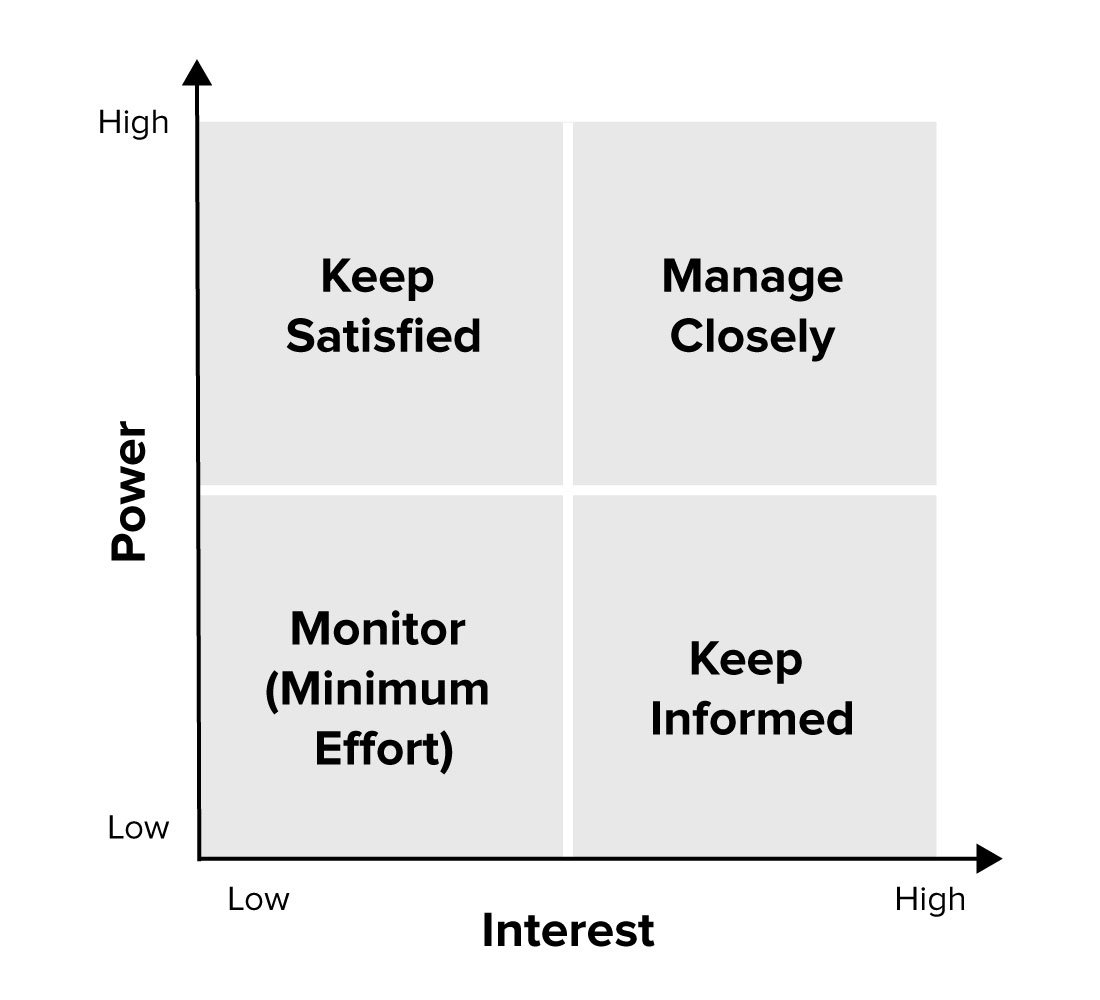
\includegraphics[width=0.5\textwidth]{power-interest.jpg}
	\caption{Power-Interest Grid}
	\label{fig:checkbox}
\end{figure}

\subsubsection{User Personas}

Once basic stakeholders are identified, user personas are used to personify them and study their cases. User personas are used in user experience (UX) design and help with building empathy for target users. In the Ideation phase, personas are used to better understand:

\begin{enumerate}
	\item Who is the ideal consumer for EIVA?
	\item What are current behaviors of those consumers?
	\item What are their needs and goals?
	\item What are the pain-points that they currently experience?
\end{enumerate}

For this research, four kinds of users are explored in different contexts based on conversations with a diverse group of consumers. The \emph{Random User Generator} service has been used to programmatically generate names --- Tanya Gonzalez, Julia Morris, Joy Fields, and Lee Henderson \cite{noauthor_random_nodate}. For profile pictures, the \emph{This Person Does Not Exist} website is used, which is a collection of AI-generated photos \cite{noauthor_this_nodate}.

\begin{wrapfigure}{l}{0.2\textwidth}
	
\includegraphics[scale=0.08]{persona-tanya.jpg}
\end{wrapfigure}

\paragraph{Tanya Gonzalez}

Tanya is a 24-year-old MSc student at a 4TU university in the Netherlands and works part-time as a student assistant. Her user environment is the classroom or library, where she spends most of her time. She enjoys trying authentic local cuisine, learning new languages, and reading Harry Potter books.

She has several professors that she wants to schedule appointments with for classes and her assistantship. Her end goal is to have a simple way to view her professors' calendars and find available time slots for meetings. Currently, this takes several email exchanges with each person and wastes a lot of time.

\begin{wrapfigure}{l}{0.2\textwidth}
	
\includegraphics[scale=0.08]{persona-julia.jpg}
\end{wrapfigure}

\paragraph{Julia Morris}

Julia is a 33-year-old freelance makeup artist based in Sydney, Australia. She is in a low-to-median income bracket and earns around AU\$45,000. She uses a point of sale (PoS) system in her makeup studio and also uses an iPad when showing her portfolio to prospective clients. She enjoys traveling and her dream is to one day release her own brand of cosmetics.

To keep track of appointments, she uses the default calendar application installed on her iPad. She currently uses WhatsApp to communicate with clients, but her end end goal is to allow them to automatically add bookings to her calendar based on her availability.

\begin{wrapfigure}{l}{0.2\textwidth}
	
\includegraphics[scale=0.08]{persona-joy.jpg}
\end{wrapfigure}

\paragraph{Joy Fields}

Joy is a 47-year-old C-level business executive at a Chicago-based multinational corporation in the financial space. She is in a very high income bracket and earns over US\$1MM per year. At work, she mostly uses a MacBook Pro, but also has email and presentation setup on her iPhone because she extensively travels as part of her job. She cares about gender equality, climate change, and data privacy. Most of her time is spent on answering emails and in meetings, for which she uses her company-provided exchange server. She has a full-time assistant, but thinks that his time would be best spent on more productive tasks.

\begin{wrapfigure}{l}{0.2\textwidth}
	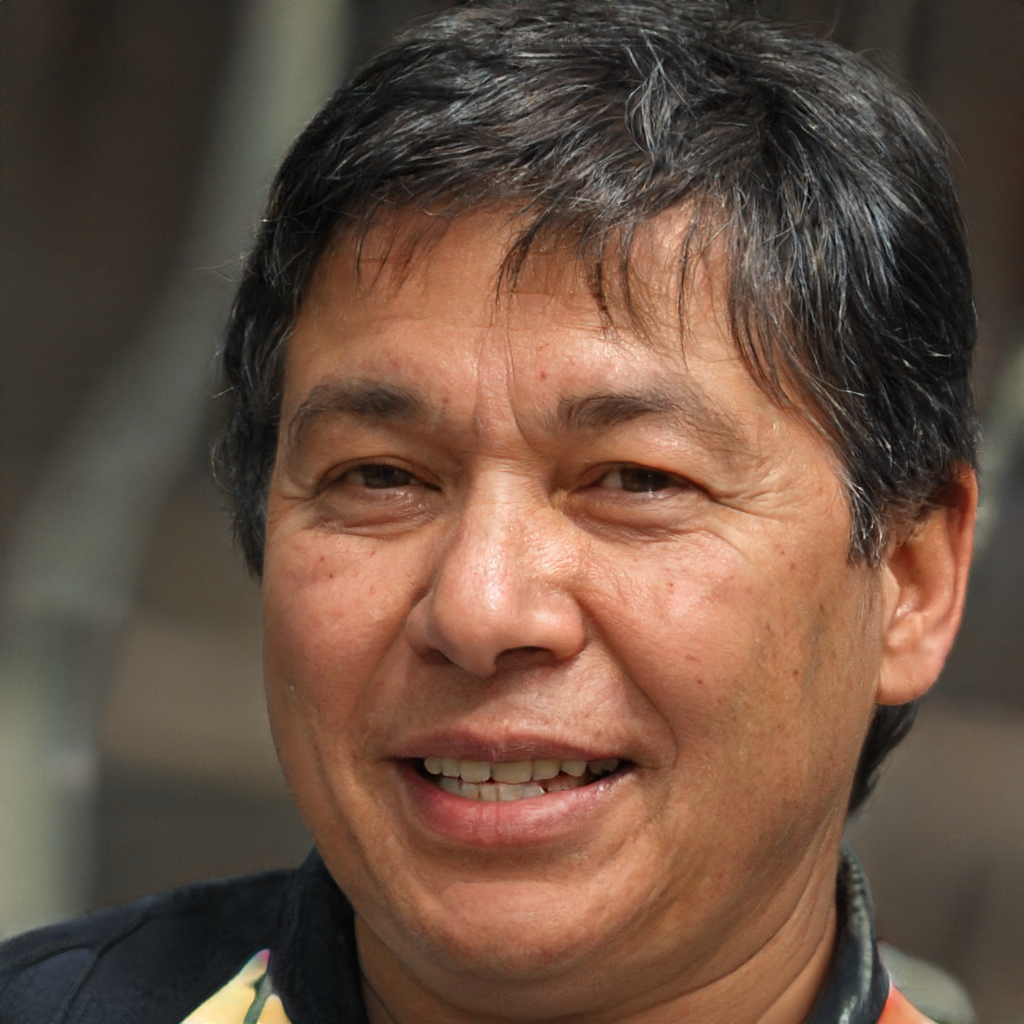
\includegraphics[scale=0.08]{persona-lee.jpg}
\end{wrapfigure}

\paragraph{Lee Henderson}

Lee is a 50 year-old startup founder who previously served in the Air Force. With his new business, he has frequent meetings with partners and investors.  His strength is in radio and navigation hardware technology, but still prefers to schedule appointments using pen and paper, a habit he has had since his days in the armed forces. He is not very keen on moving to a digital system, but considers himself open-minded and likes trying new products.

\begin{table}[!htb]
	\begin{minipage}{1\linewidth}
		\caption{Comparison of User Personas}
		\centering
		\begin{tabular}{llll}
			\hline
			\textbf{User} & \textbf{Income} & \textbf{Current Behavior} & \textbf{Requirement}         \\
			\hline
			Tanya         & Low             & Email & Appointments with professors \\
			Julia         & Medium          & WhatsApp & Managing time slots          \\
			Joy           & High            & Personal Assistant & Calls with team              \\
			Lee           & Medium          & Pen-and-paper & Meetings with partners       \\
			\hline
		\end{tabular}
	\end{minipage}%
\end{table}

Though the use cases for each persona are different, they all fall under the umbrella of ``I want a better, more automated way of scheduling appointments." For Tanya, it is to interact with professors; for Julia, with clients; for Joy, with her team; and for Lee, with his business partners. With an automated virtual agent that can schedule appointments without input from users, a significant part of all of their problems may be solved.

\subsection{Assistant Architecture}

\begin{wrapfigure}{l}{0.5\textwidth}\centering
	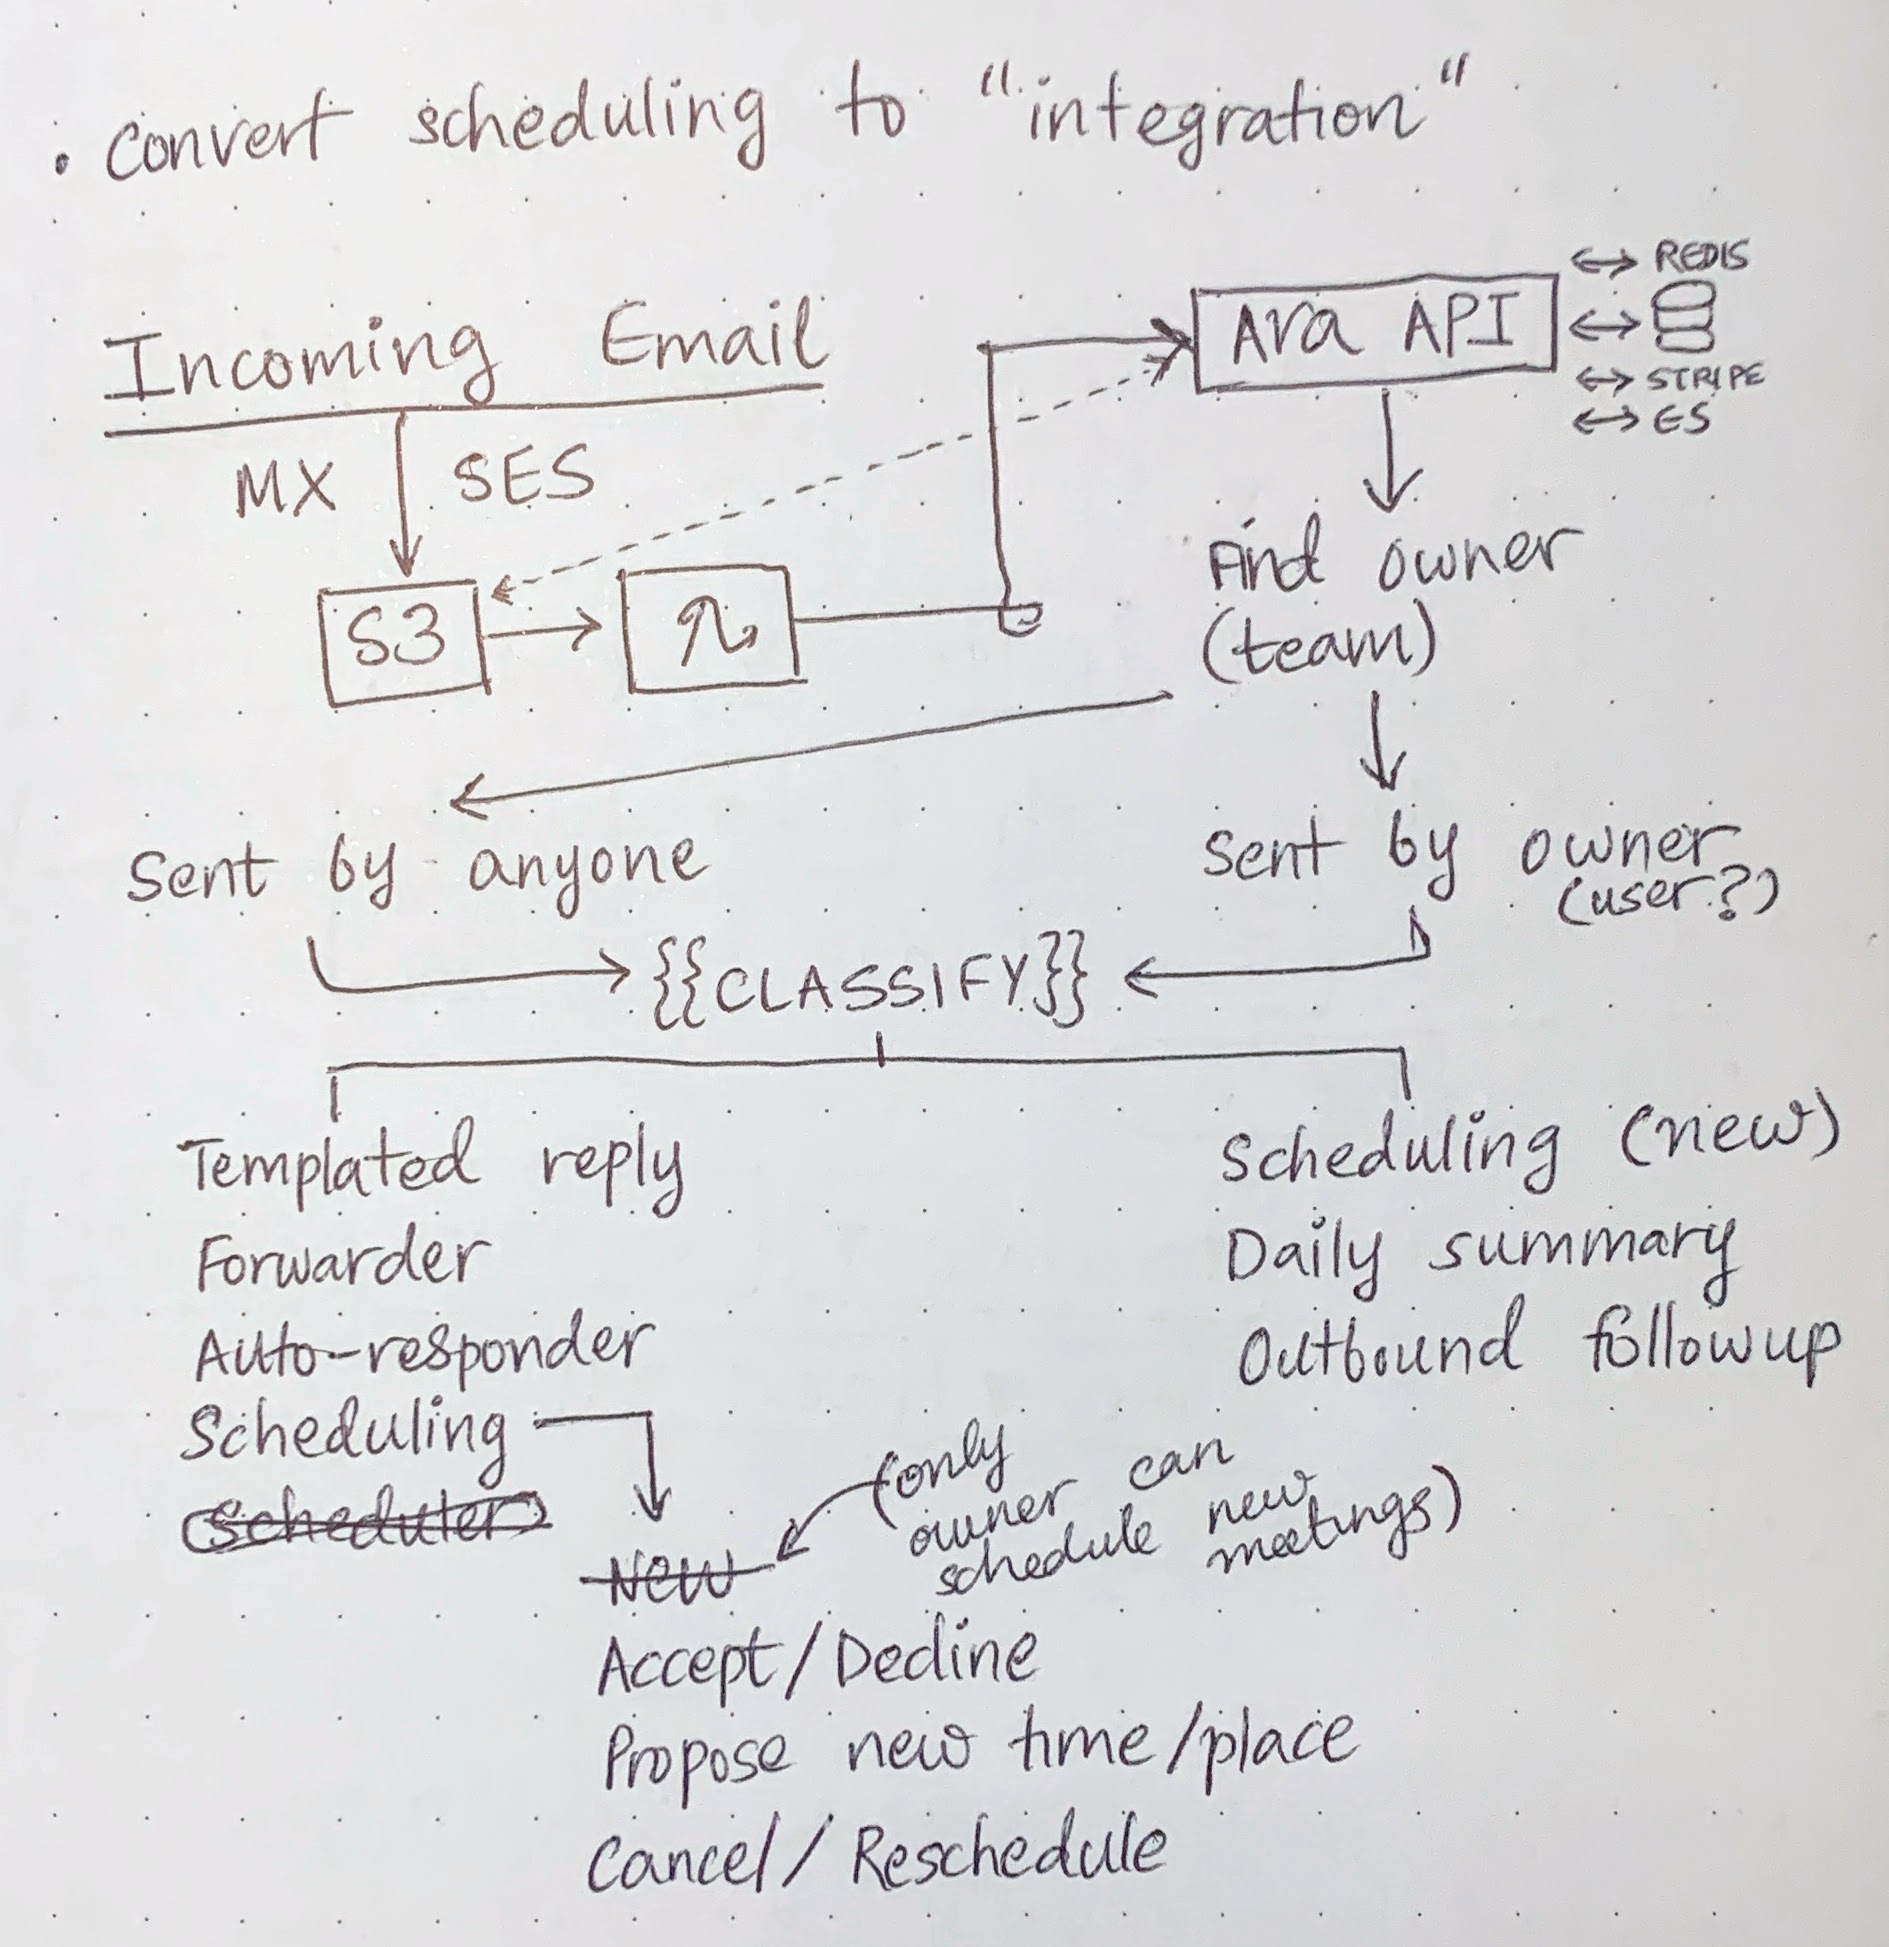
\includegraphics[scale=0.097]{drawing-all-process.jpg}
	\caption{Email Process Ideation}
\end{wrapfigure}

A pen-and-paper exploration of the the entire process from receiving a new email, understanding it, and performing an action, was conducted. In Figure X, each intent (such as scheduling an appointment, forwarding an email, etc.), is performed based on the classification of the incoming email.

Here, the process of receiving an email, saving the contents, and invoking a serverless function is visualized. The diagram also showcases the connection of the API with other services like a database and payment gateway.

The API then finds the owner of the team the email was addressed to and whether or not the owner themselves sent the email. After classification, one of several processes are queued.

In a separate exploration, a rule-based approach was chosen instead of intent-based classification to understand an incoming email. In Figure 2, a user interface was mocked up wherein consumers could set custom rules to perform action when new emails are received. In the example, there are three types of UI elements --- select dropdowns, text inputs, and buttons.

\begin{wrapfigure}{r}{0.5\textwidth}\centering
	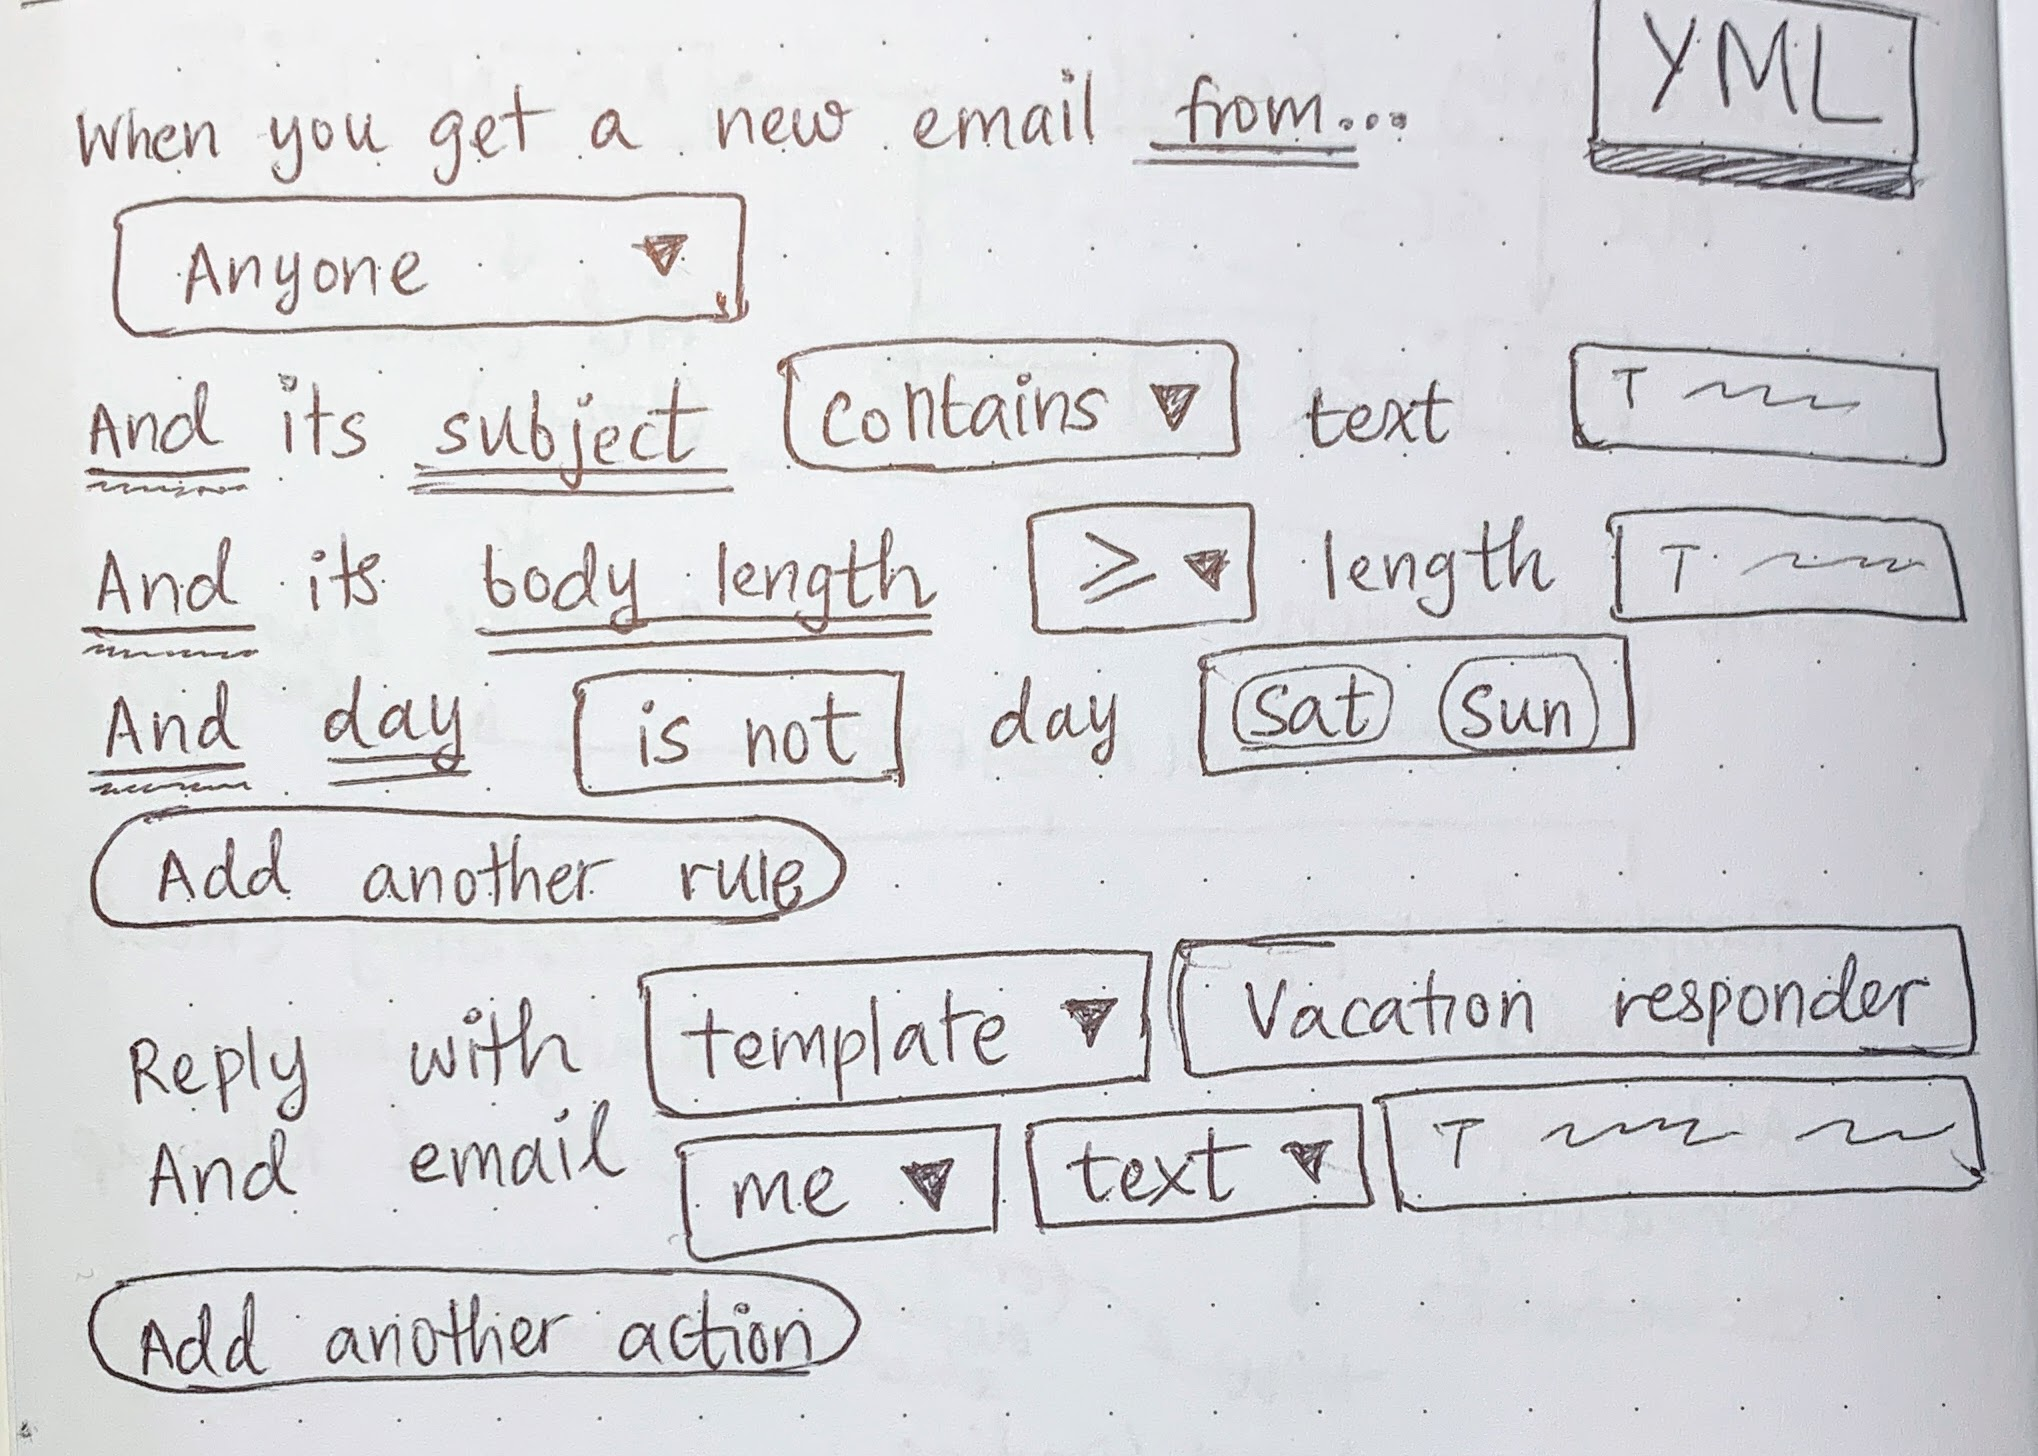
\includegraphics[scale=0.092]{drawing-rules-ui.jpg}
	\caption{Rule-based Process Ideation}
\end{wrapfigure}

In the example UI, the rule is "When you get an email from \emph{anyone}, \emph{and} its \emph{subject} \emph{contains} the text (input), \emph{and} its \emph{body length} \emph{is greater than or equal to} (length), \emph{and} the \emph{day} \emph{is not} one of the days \emph{Sat, Sun}, automatically reply with \emph{template} \emph{Vacation responder} and also email \emph{me} with the (text). Complicated rules such as these can be generated by the proposed UI, allowing users to automate several different types of repetitive email tasks.

\subsection{Web App UI}

For setting preferences and managing scheduled appointments, a functional and easy-to-use companion web application must be developed. In Figure 4, early wireframes of the web app are designed, using both desktop and smartphone form factors. After creating an account and verifying their email, users can log in and will be taken to the onboarding interface to set up their assistant. Then, users are taken to the Dashboard page with an overview of their meetings, and can choose to go to the Settings page to configure their preferences.

\begin{figure}[h]
	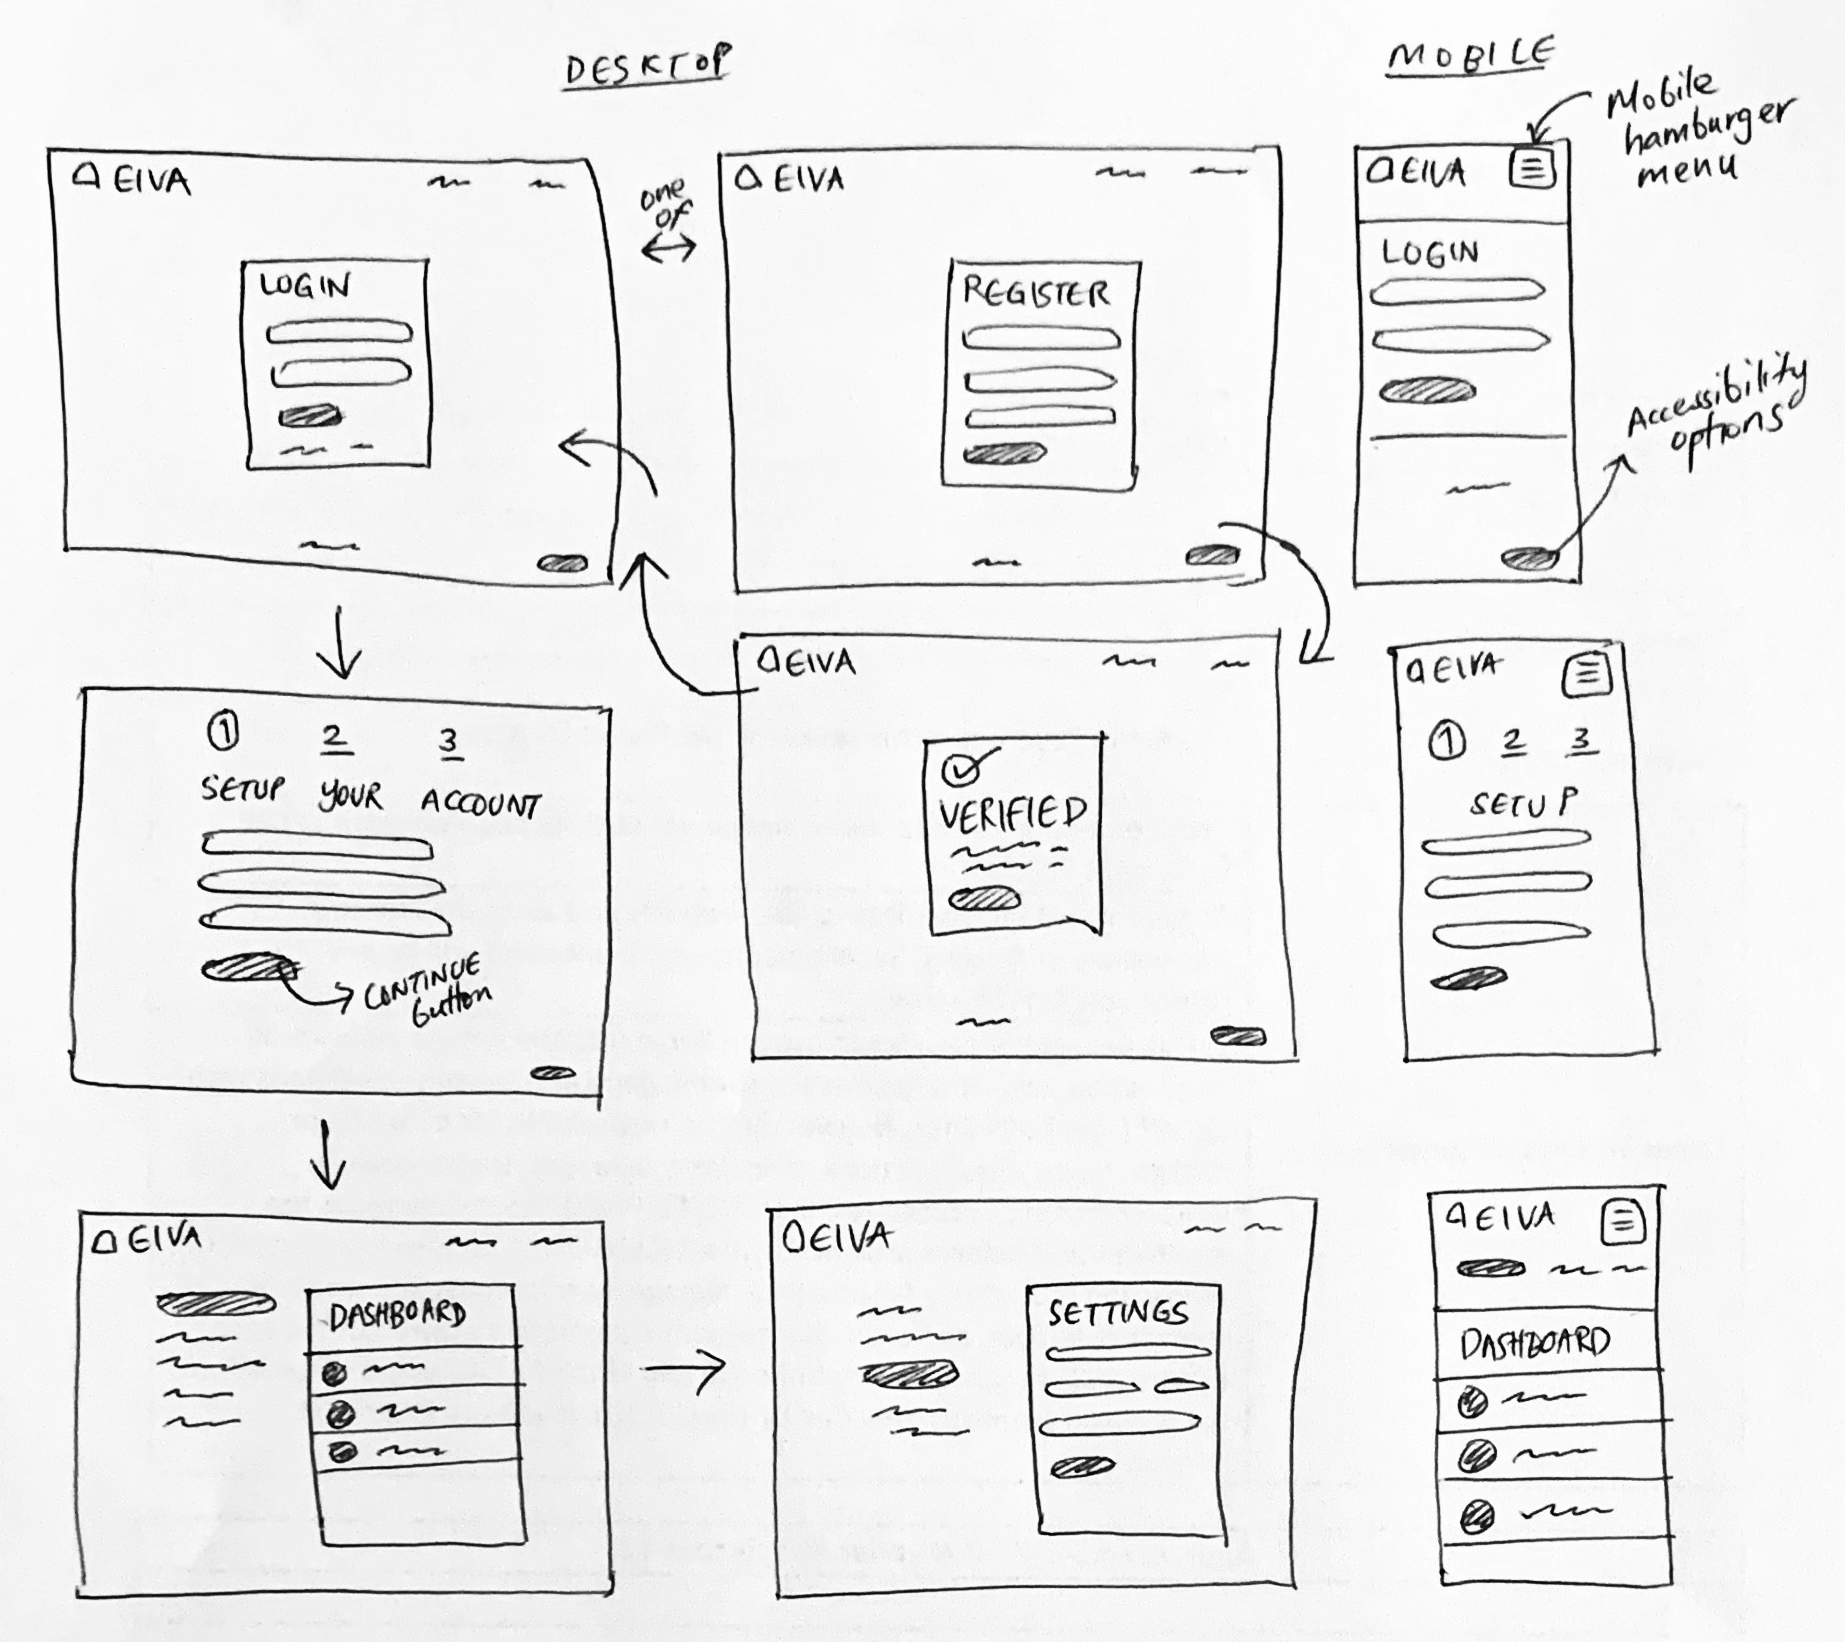
\includegraphics[width=\textwidth]{drawing-ui.jpg}
	\caption{Webpage Wireframes on Paper}
\end{figure}

Figure 4 also shows a two-column layout for desktop pages, with the left sidebar for the primary navigation and a card for the main content. On mobile, a hamburger menu is used with the same design. An accessibility options floating button is also shown on the bottom-right corner of each design. In Figure 5 and 6, more detailed wireframes are drawn using a mobile stencil on paper.
 
 \begin{figure}
	\centering
	\begin{minipage}{.5\textwidth}
		\centering
		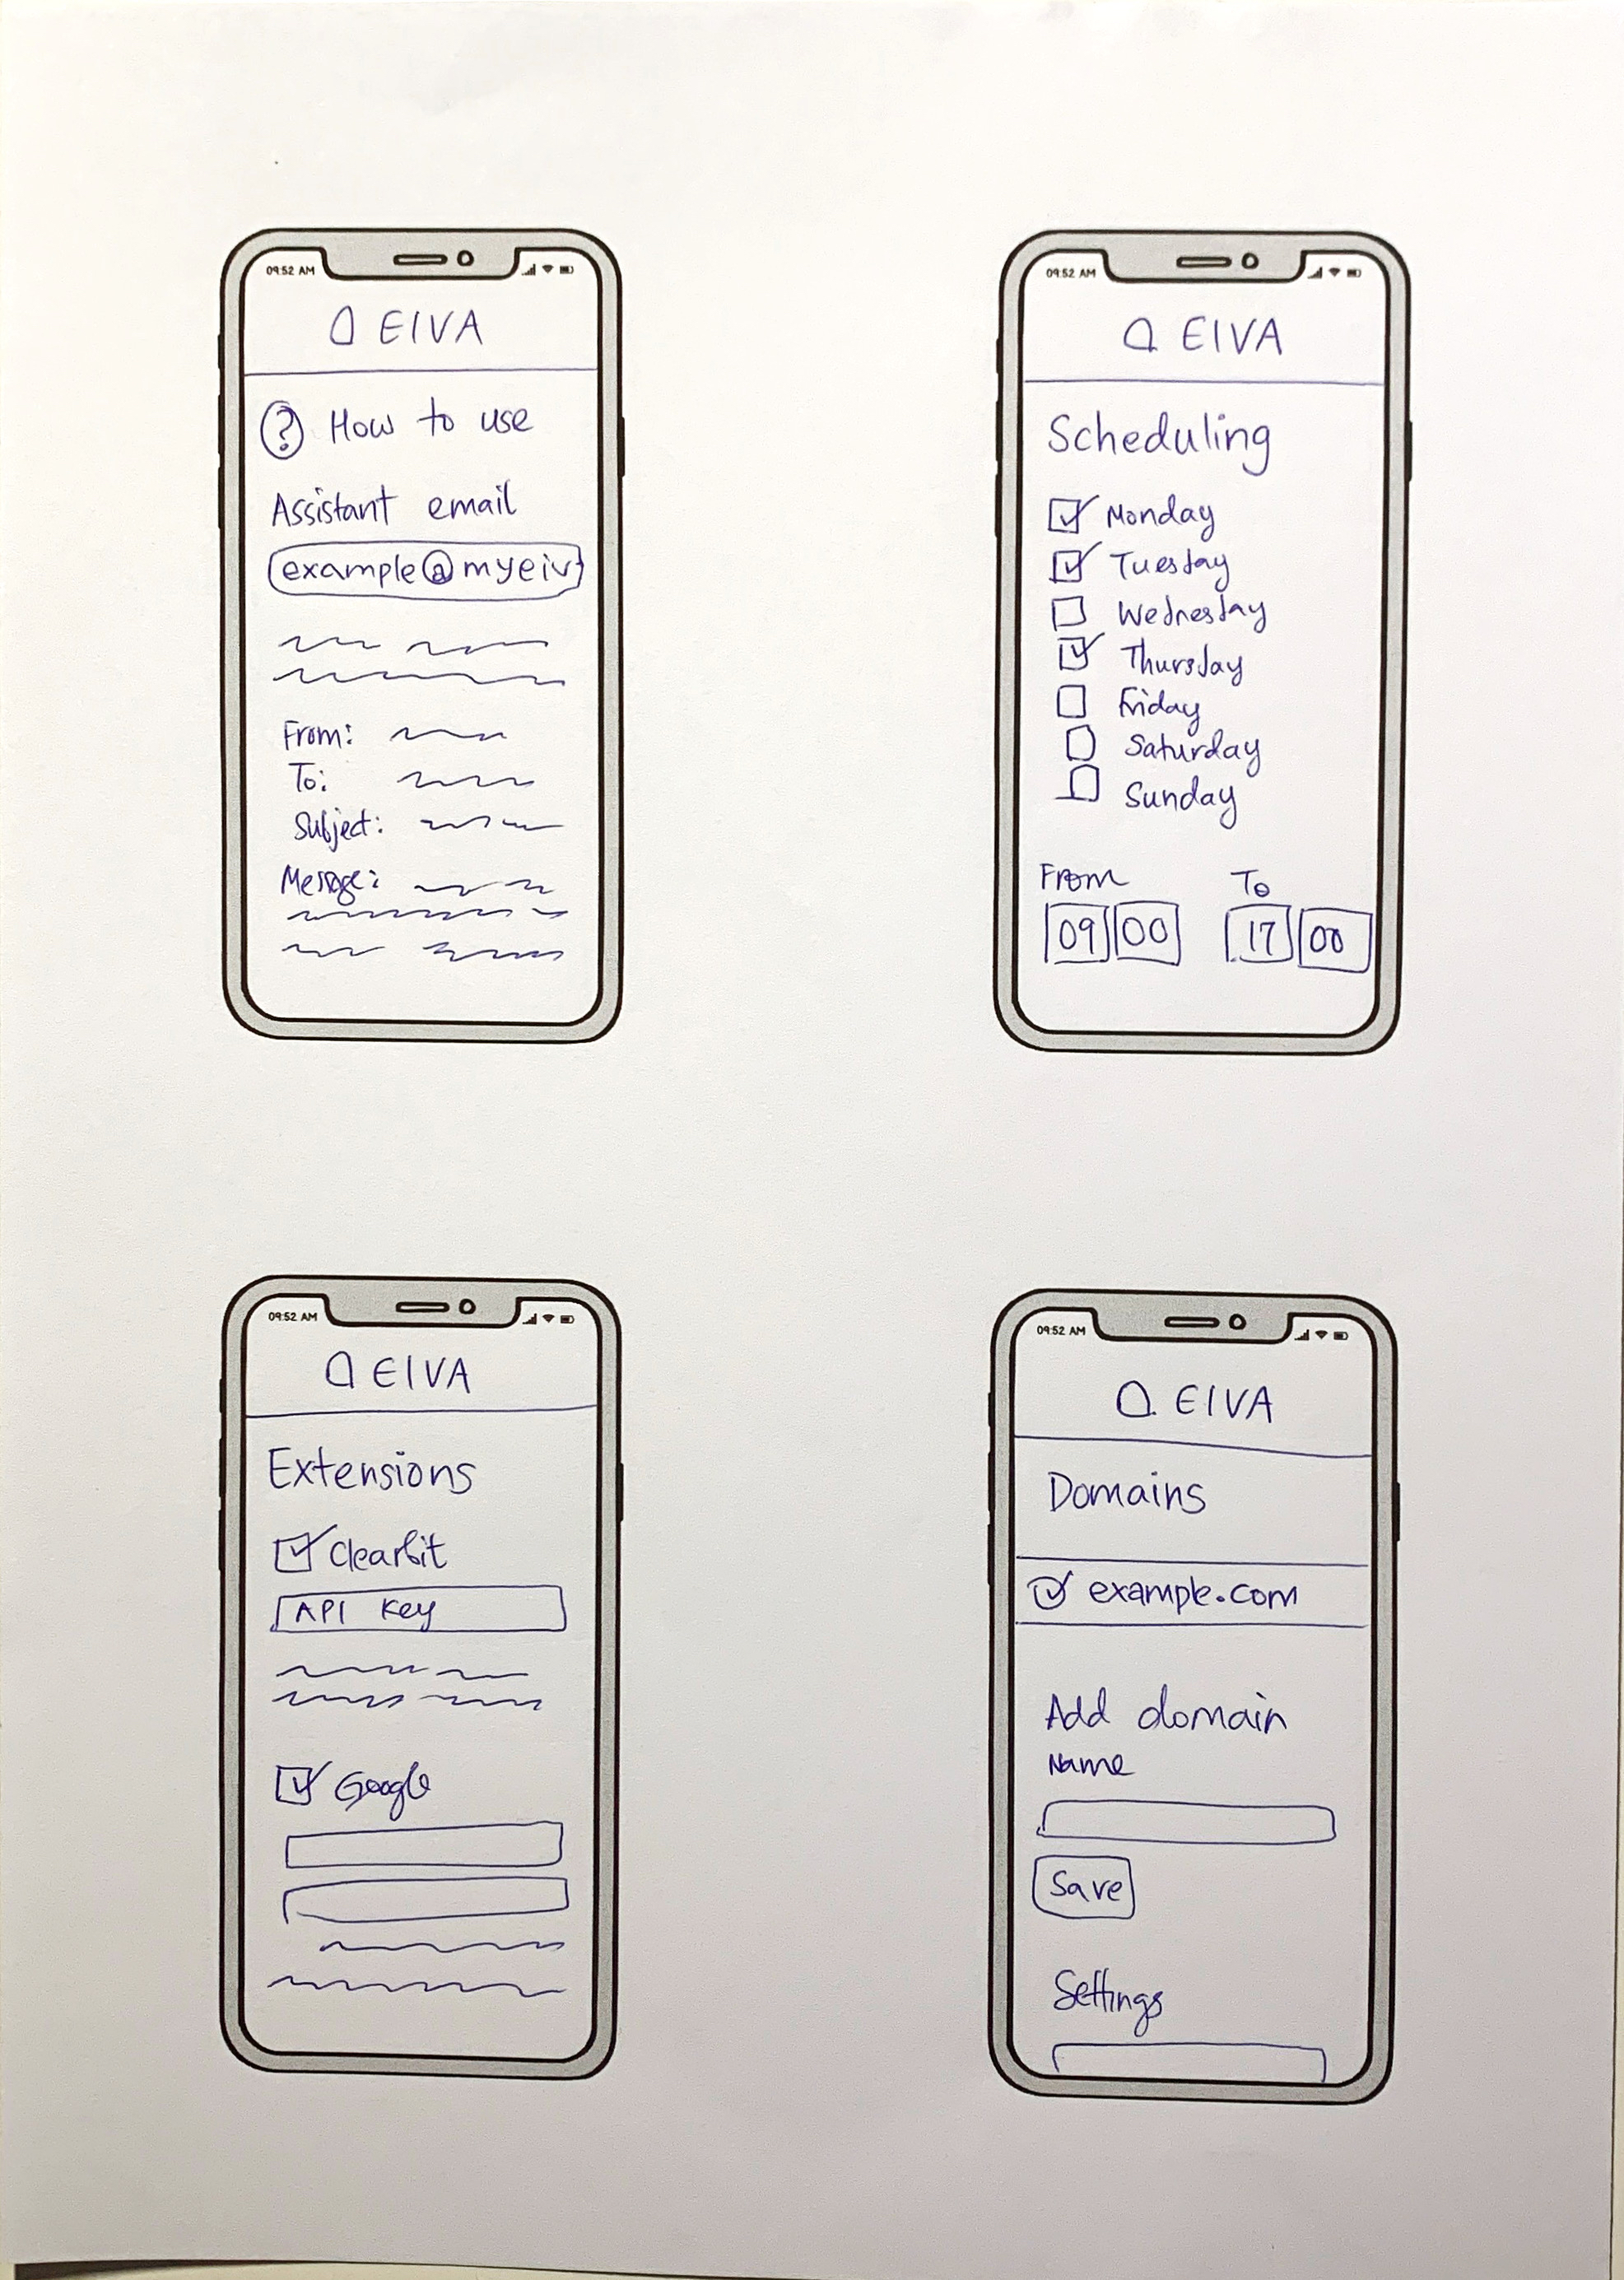
\includegraphics[width=1\linewidth]{drawing-phone-1.jpg}
		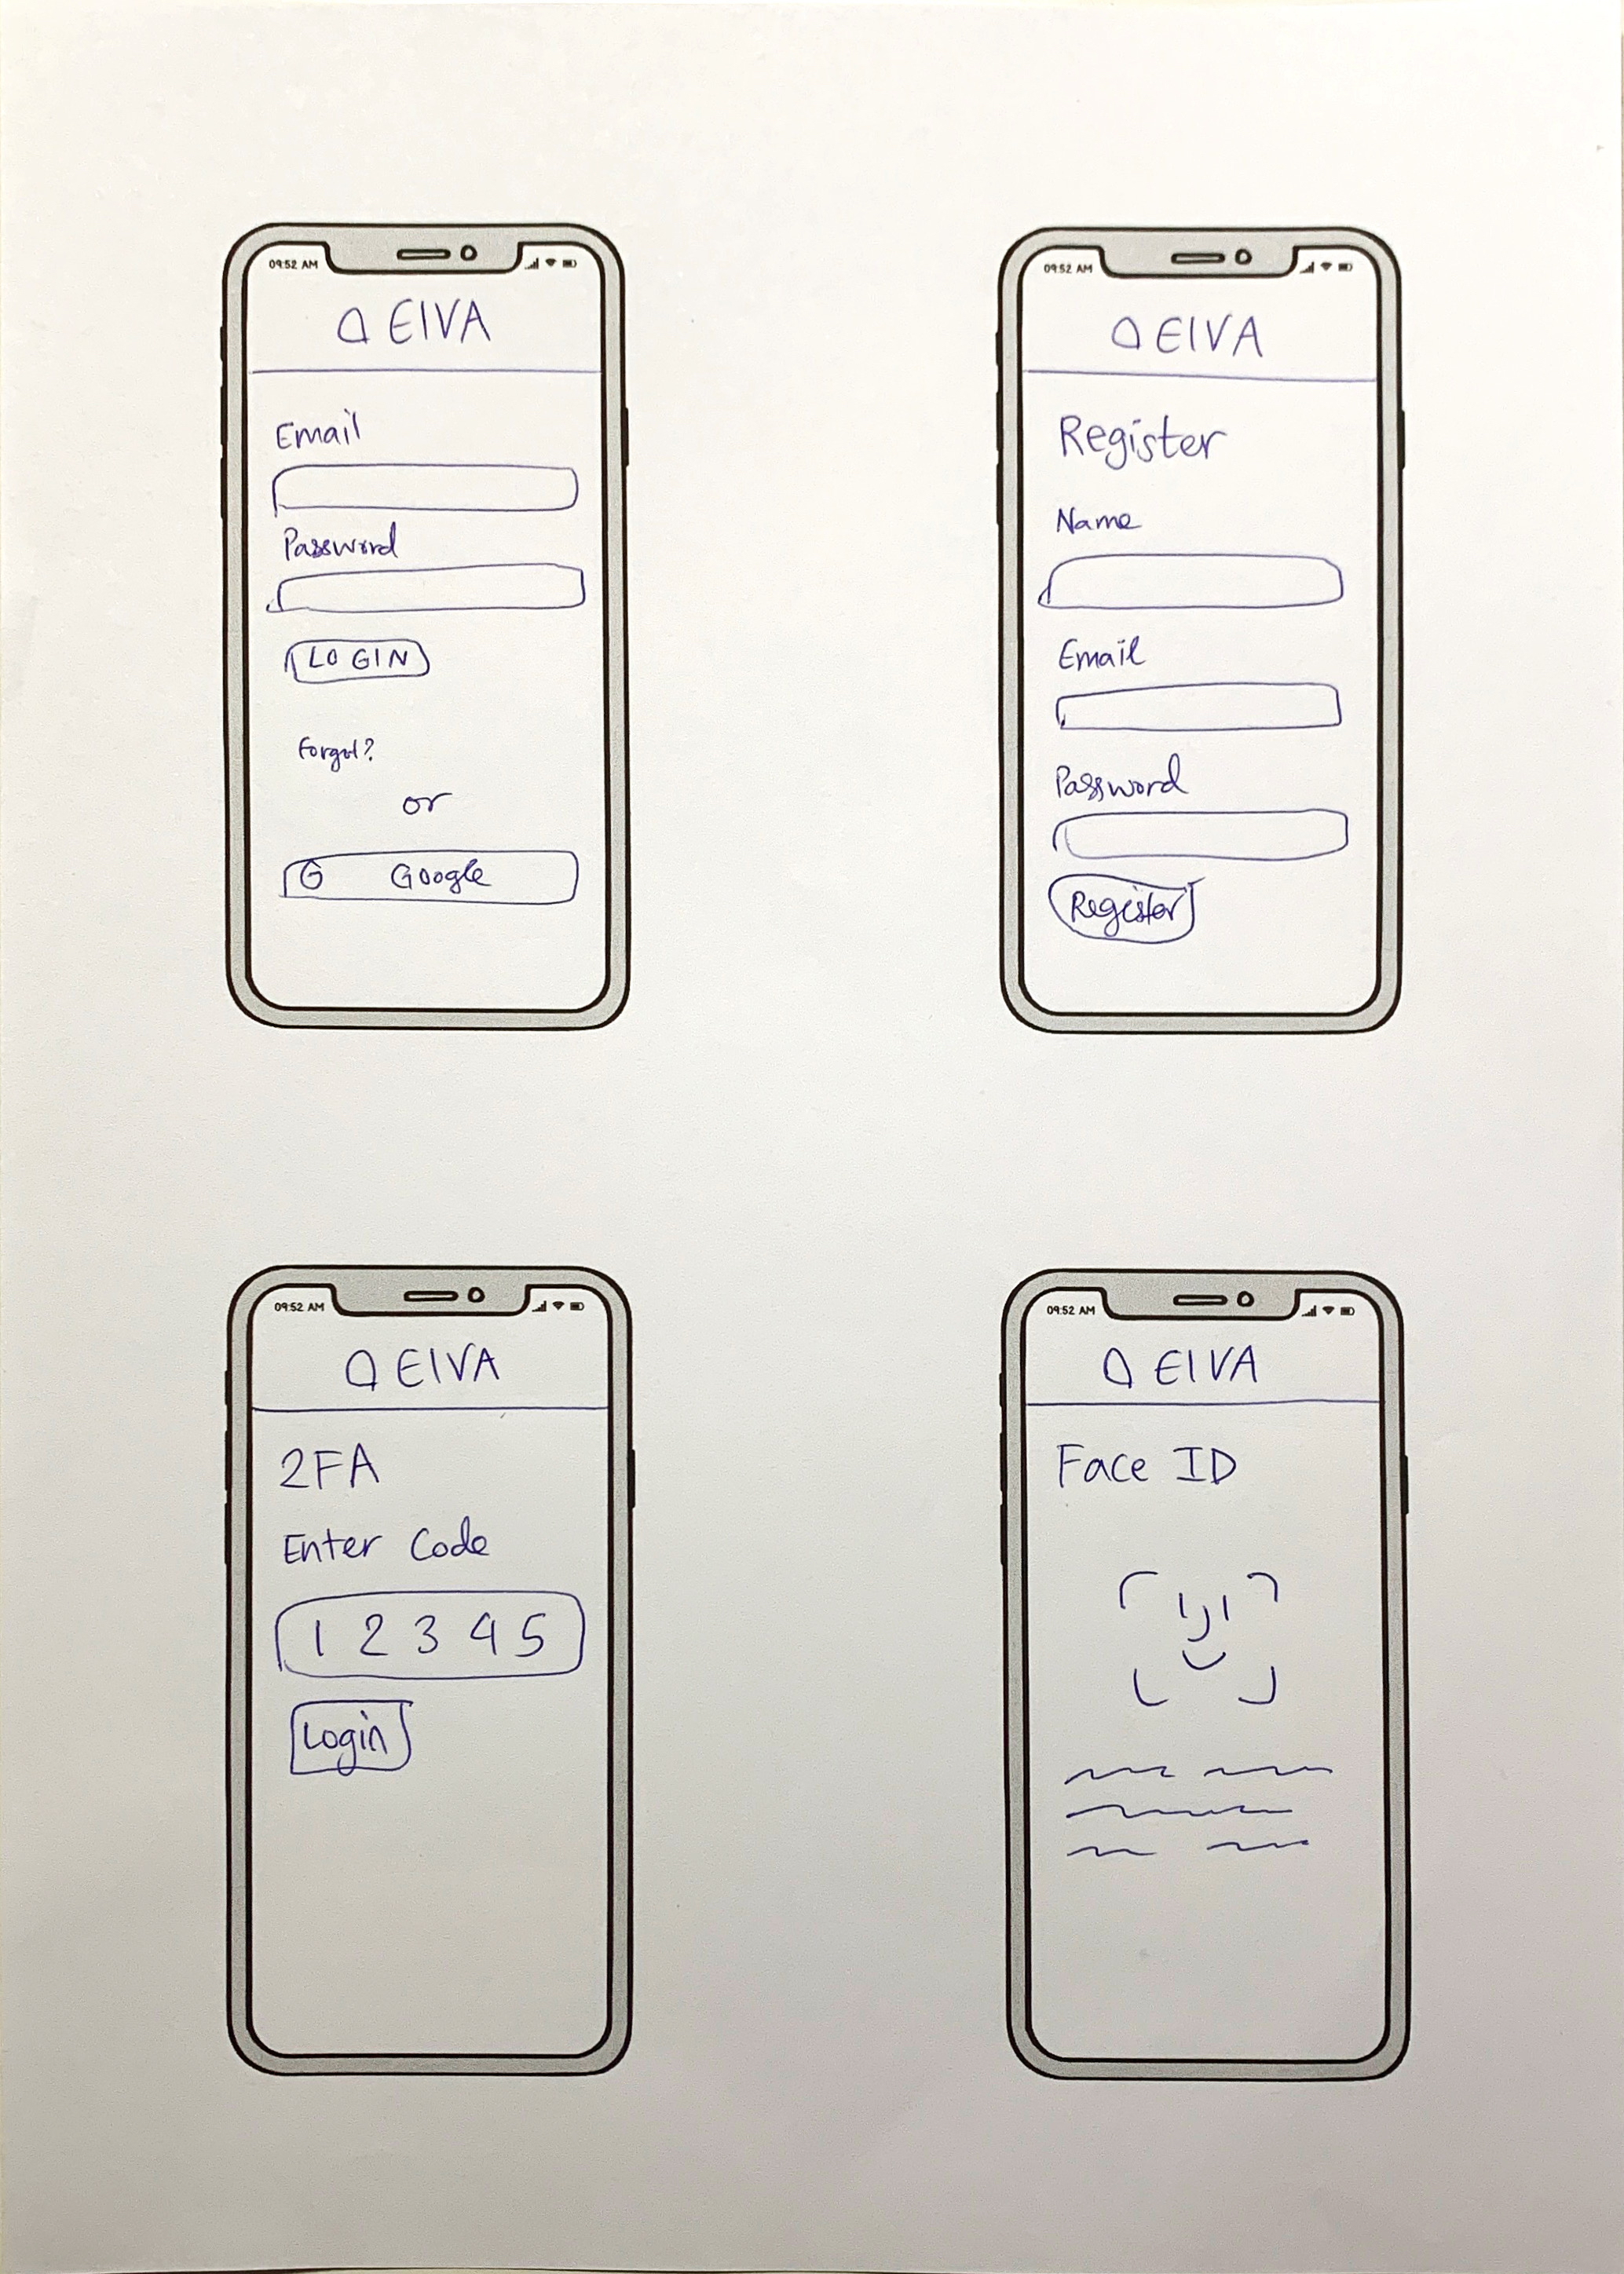
\includegraphics[width=1\linewidth]{drawing-phone-2.jpg}
	\end{minipage}%
	\begin{minipage}{.5\textwidth}
		\centering
		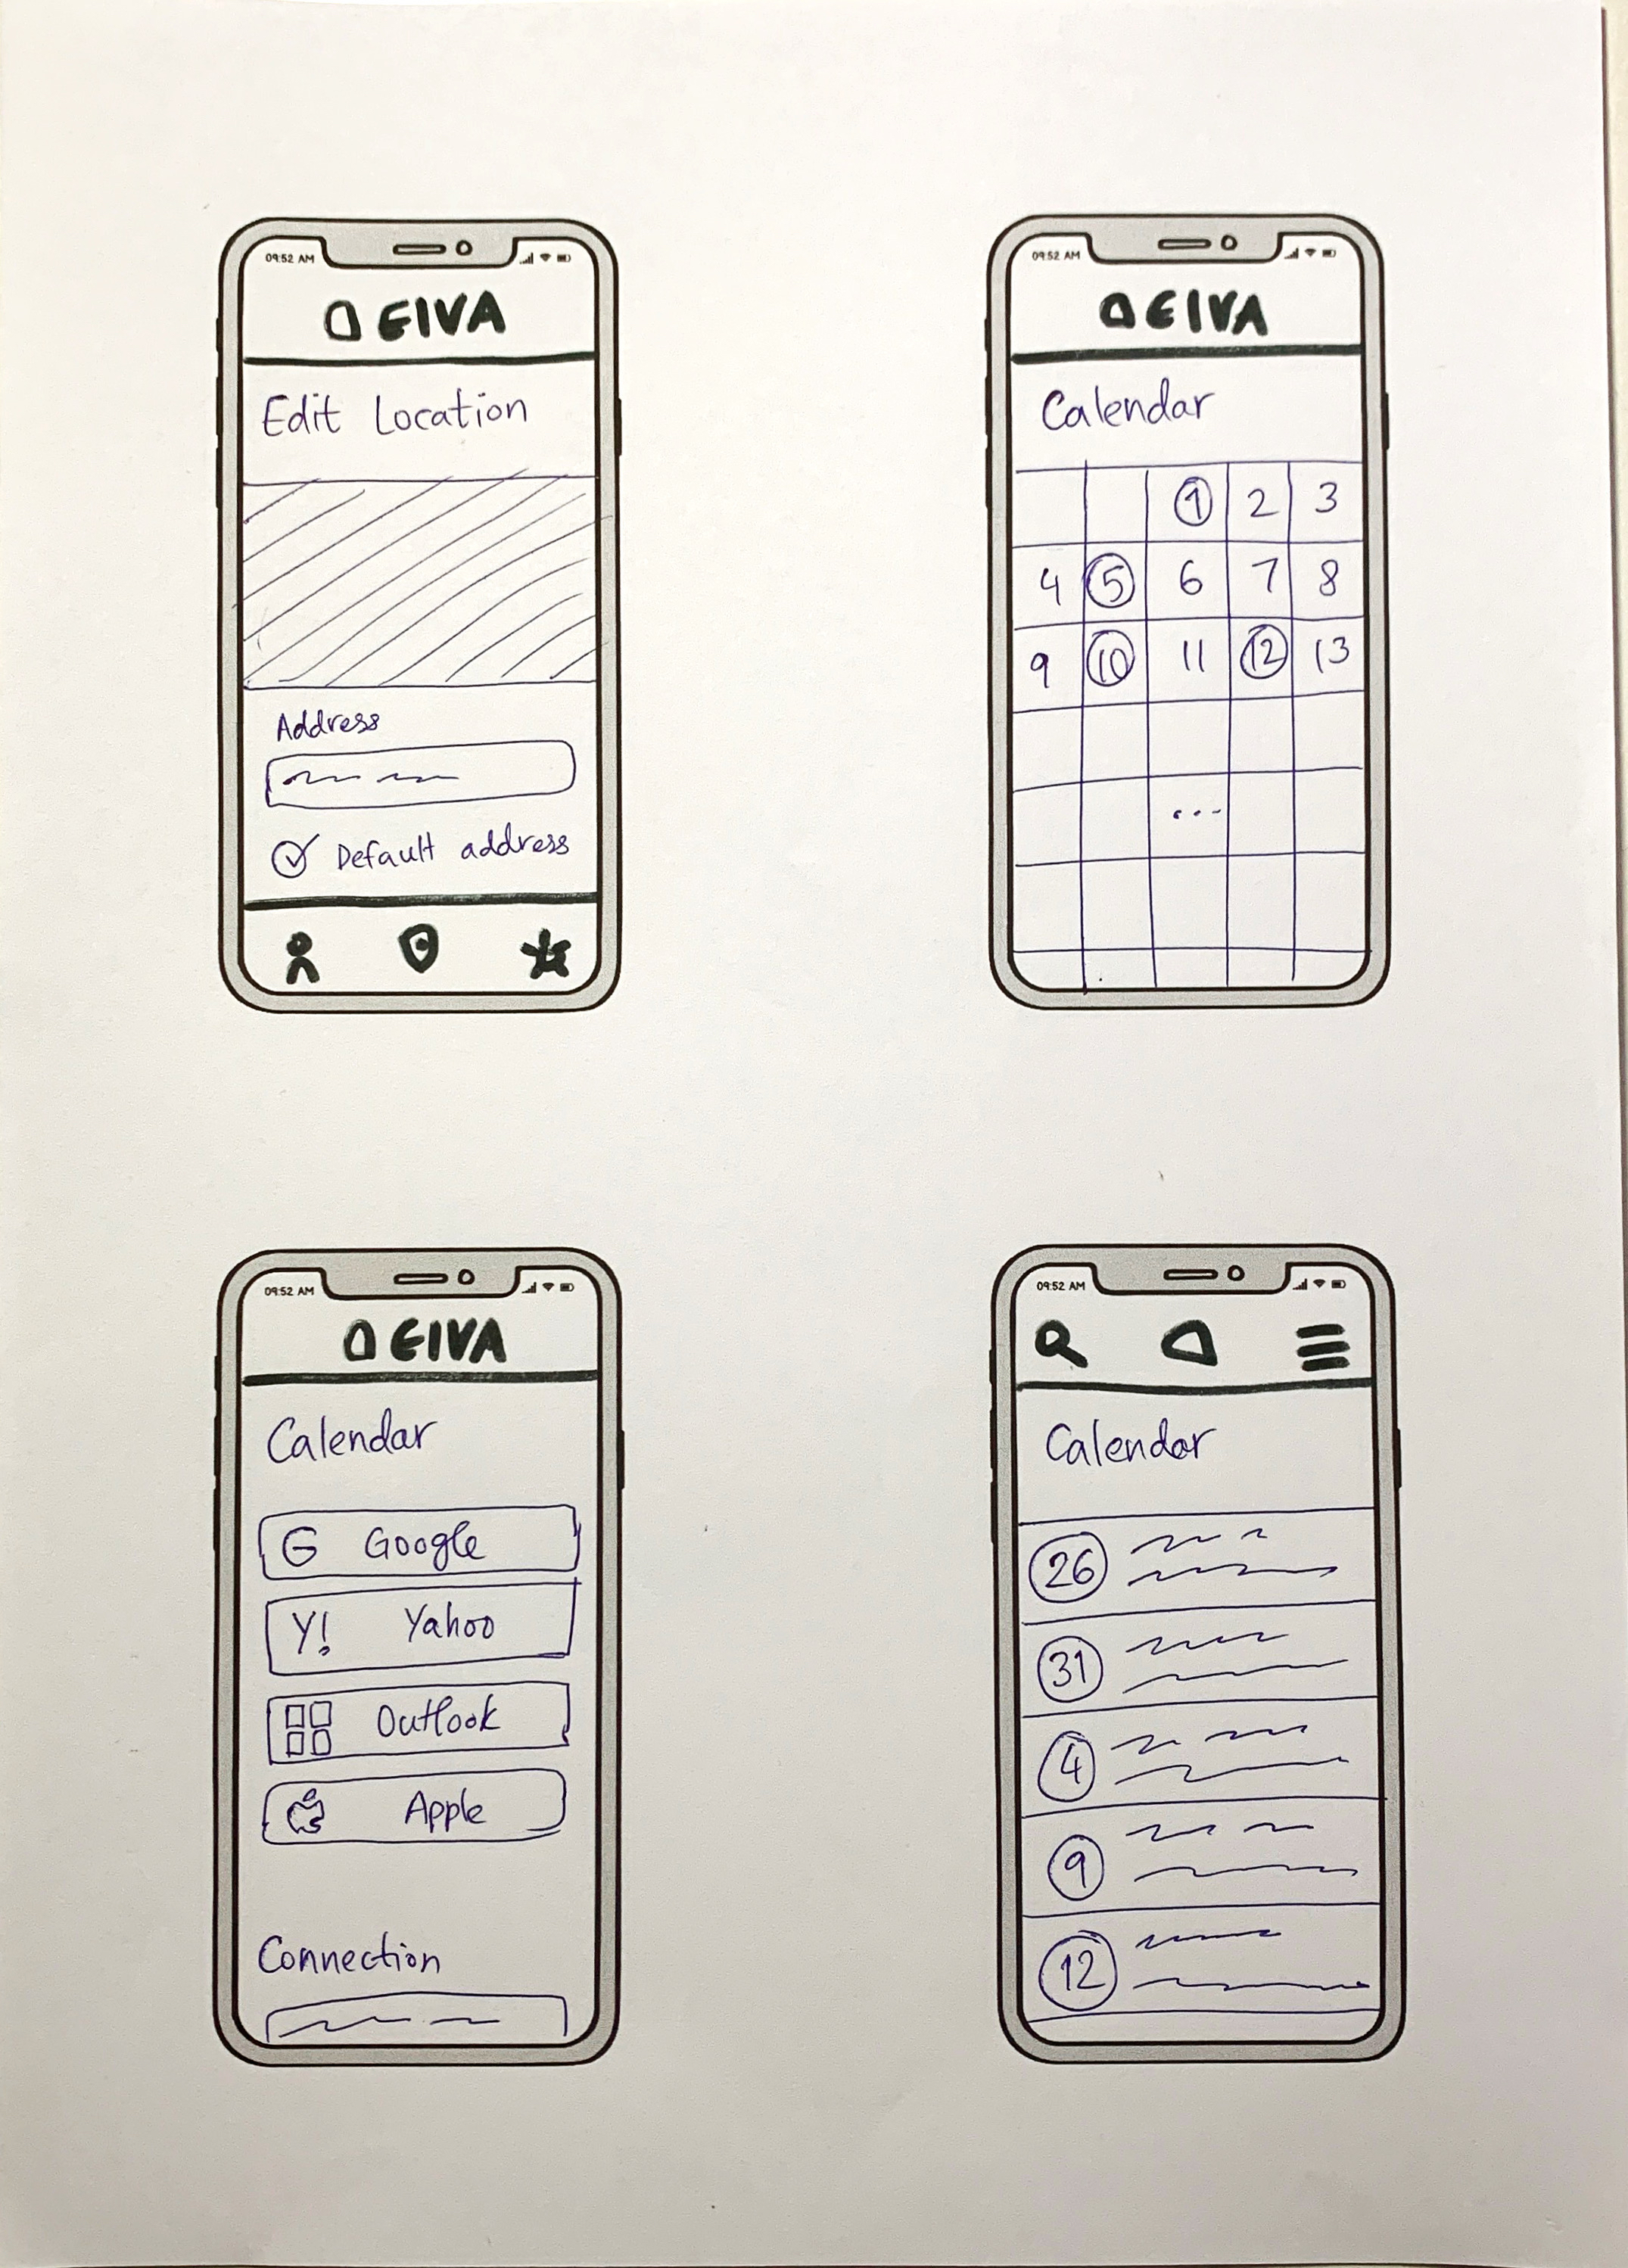
\includegraphics[width=1\linewidth]{drawing-phone-3.jpg}
		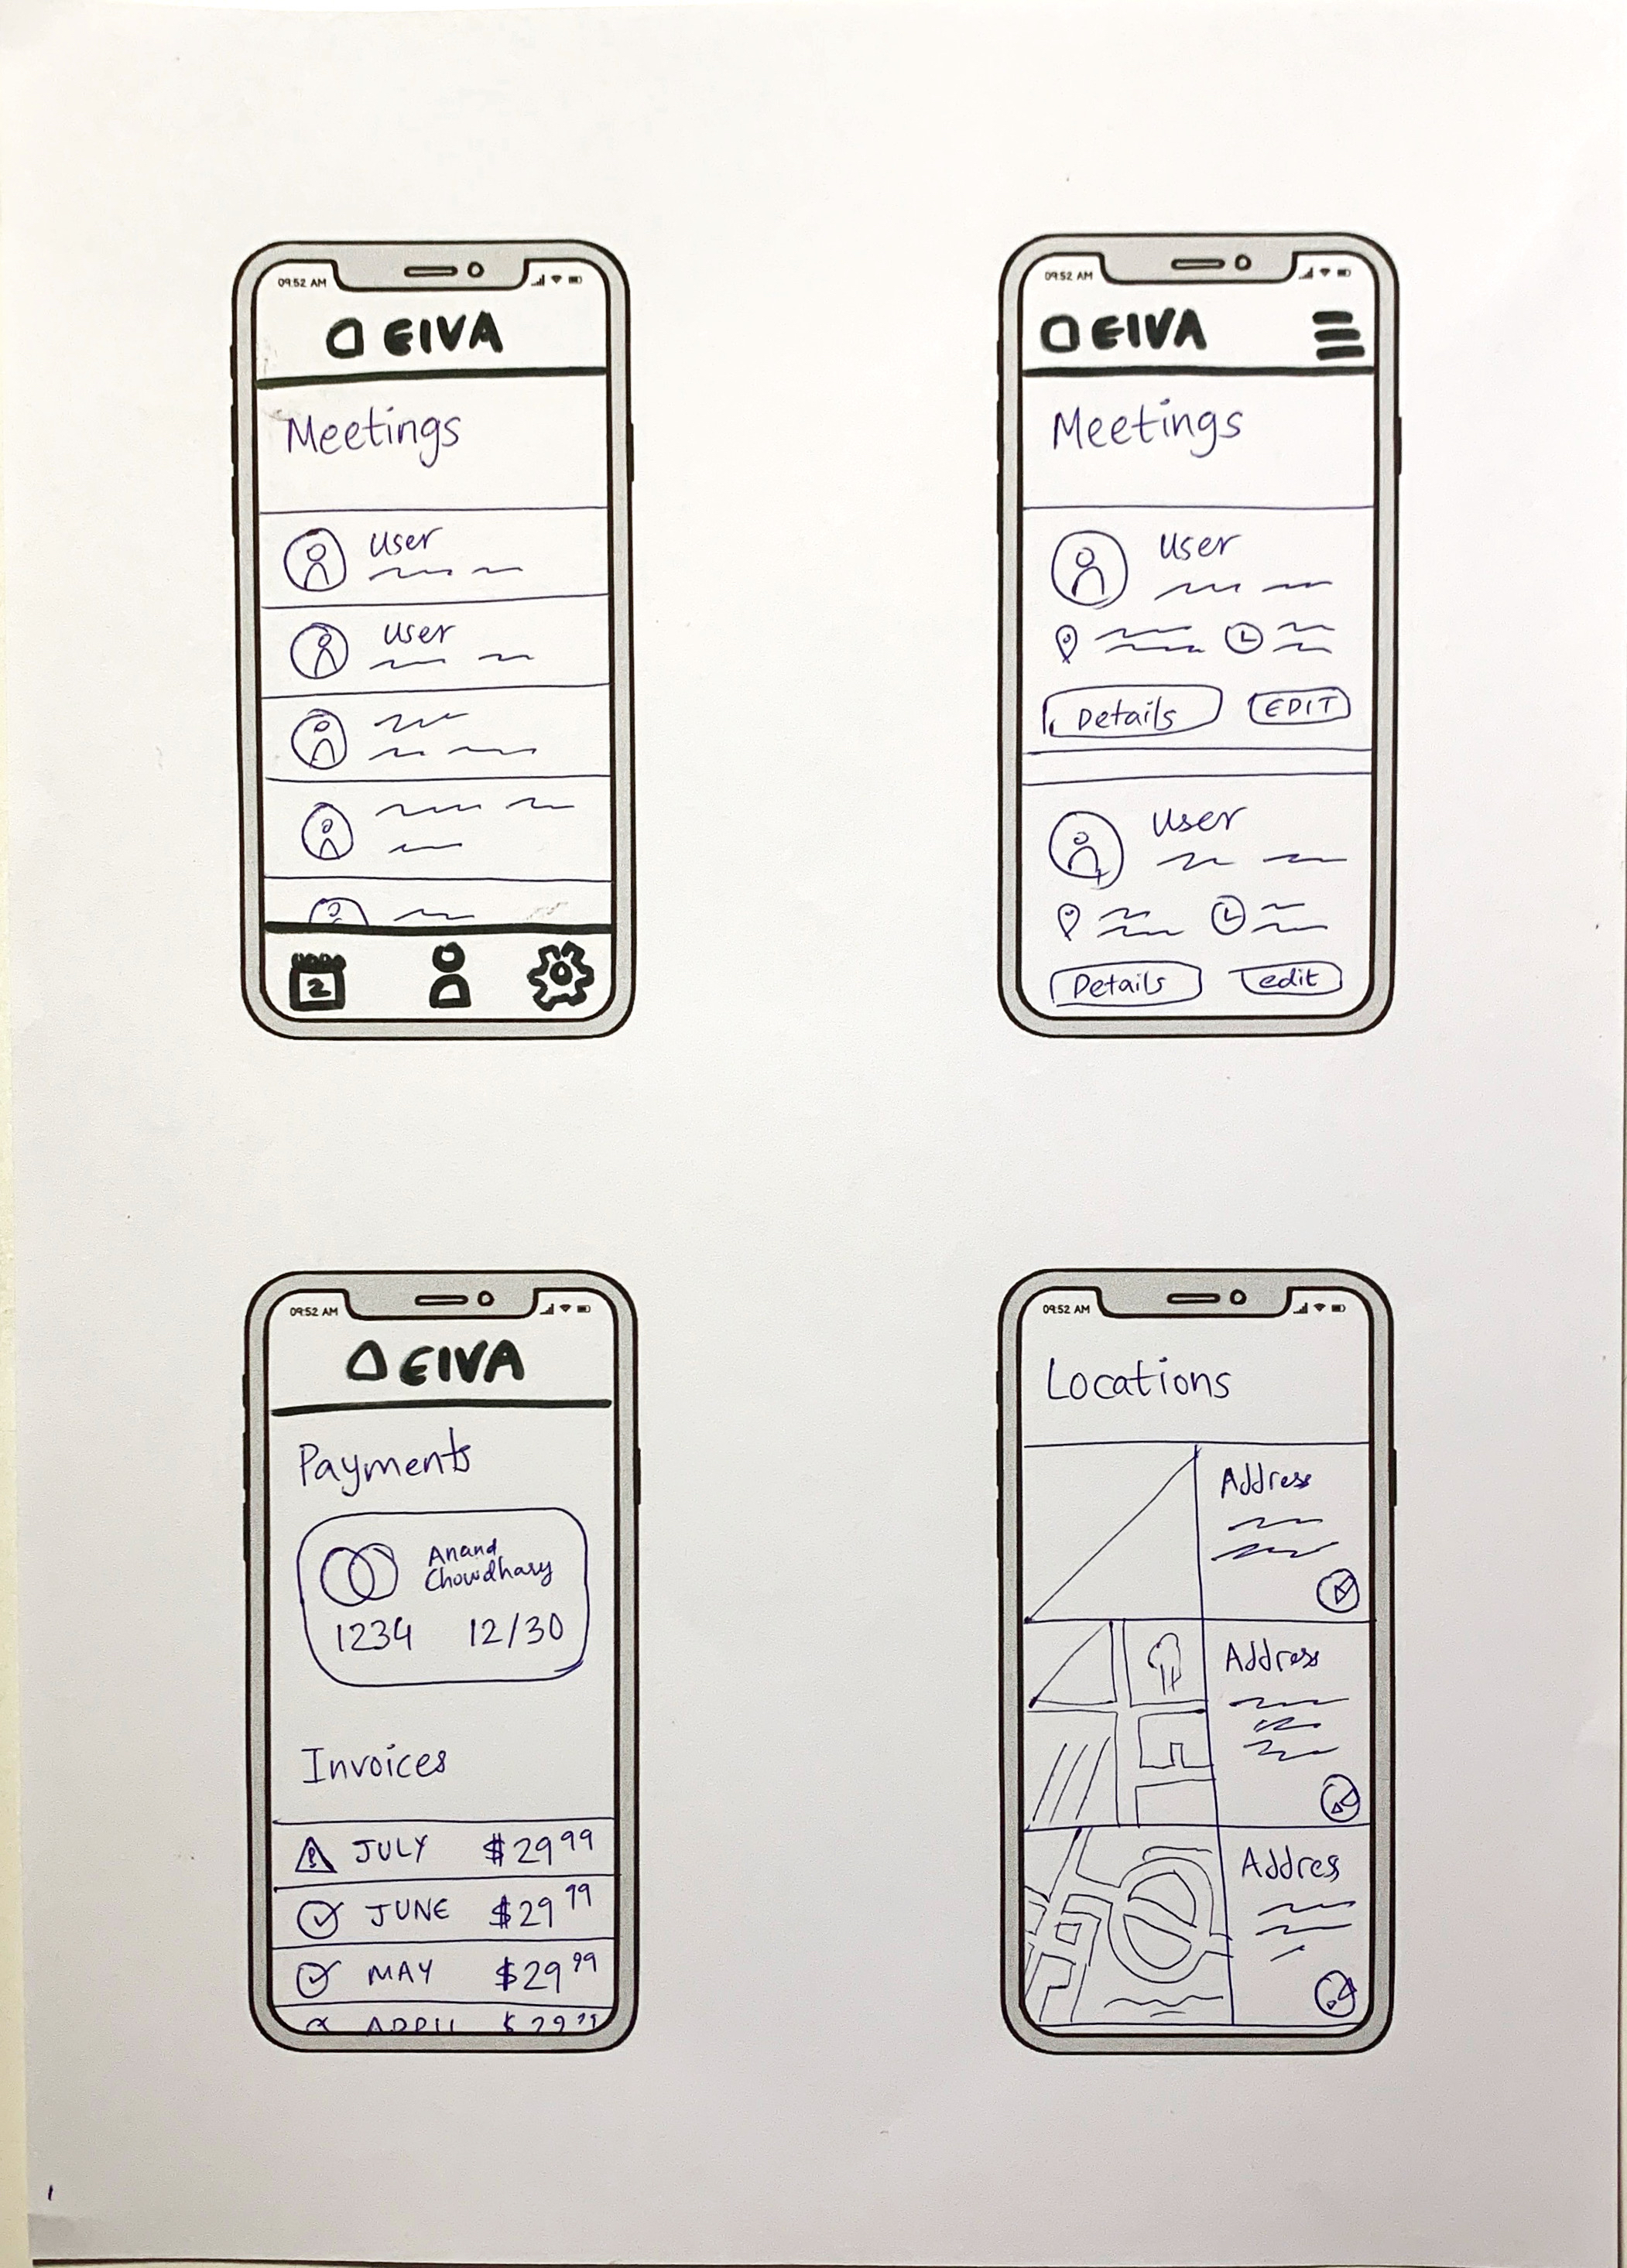
\includegraphics[width=1\linewidth]{drawing-phone-4.jpg}
	\end{minipage}
	\caption{Mobile Wireframes on Paper}
\end{figure}

 A basic version of each required interface is shown in Figure 6, with the following interfaces from left to right and top to bottom:
\begin{enumerate}
	\item How to Use: Help new users understand how to communicate with their assistant over email
	\item Scheduling: Set scheduling preferences like active days and working hours
	\item Login: Sign in to an account using email and password or Google
	\item Register: Create a new account with name, email, and password
	\item Extensions: Advanced integrations like custom API keys and authentication for Clearbit or Google Calendar
	\item Domains: Manage verified domain names for team accounts
	\item 2FA: Post-login verification for two-factor authentication
	\item Face ID: Optional login verification using Apple's Face ID
	\item Edit Location: Map interface to update location details
	\item Calendar: Overview interface for meetings in the coming month
	\item Meetings: A list of upcoming meetings with user avatars
	\item Meetings: An expanded card interface for upcoming meetings
	\item Calendar: Connections with various calendaring services
	\item Calendar: List-view for upcoming appointments
	\item Payments: Invoices and credit card details for SaaS payments
	\item Locations: List of saves locations with map interface
\end{enumerate}

\begin{wrapfigure}{l}{0.4\textwidth}\centering
	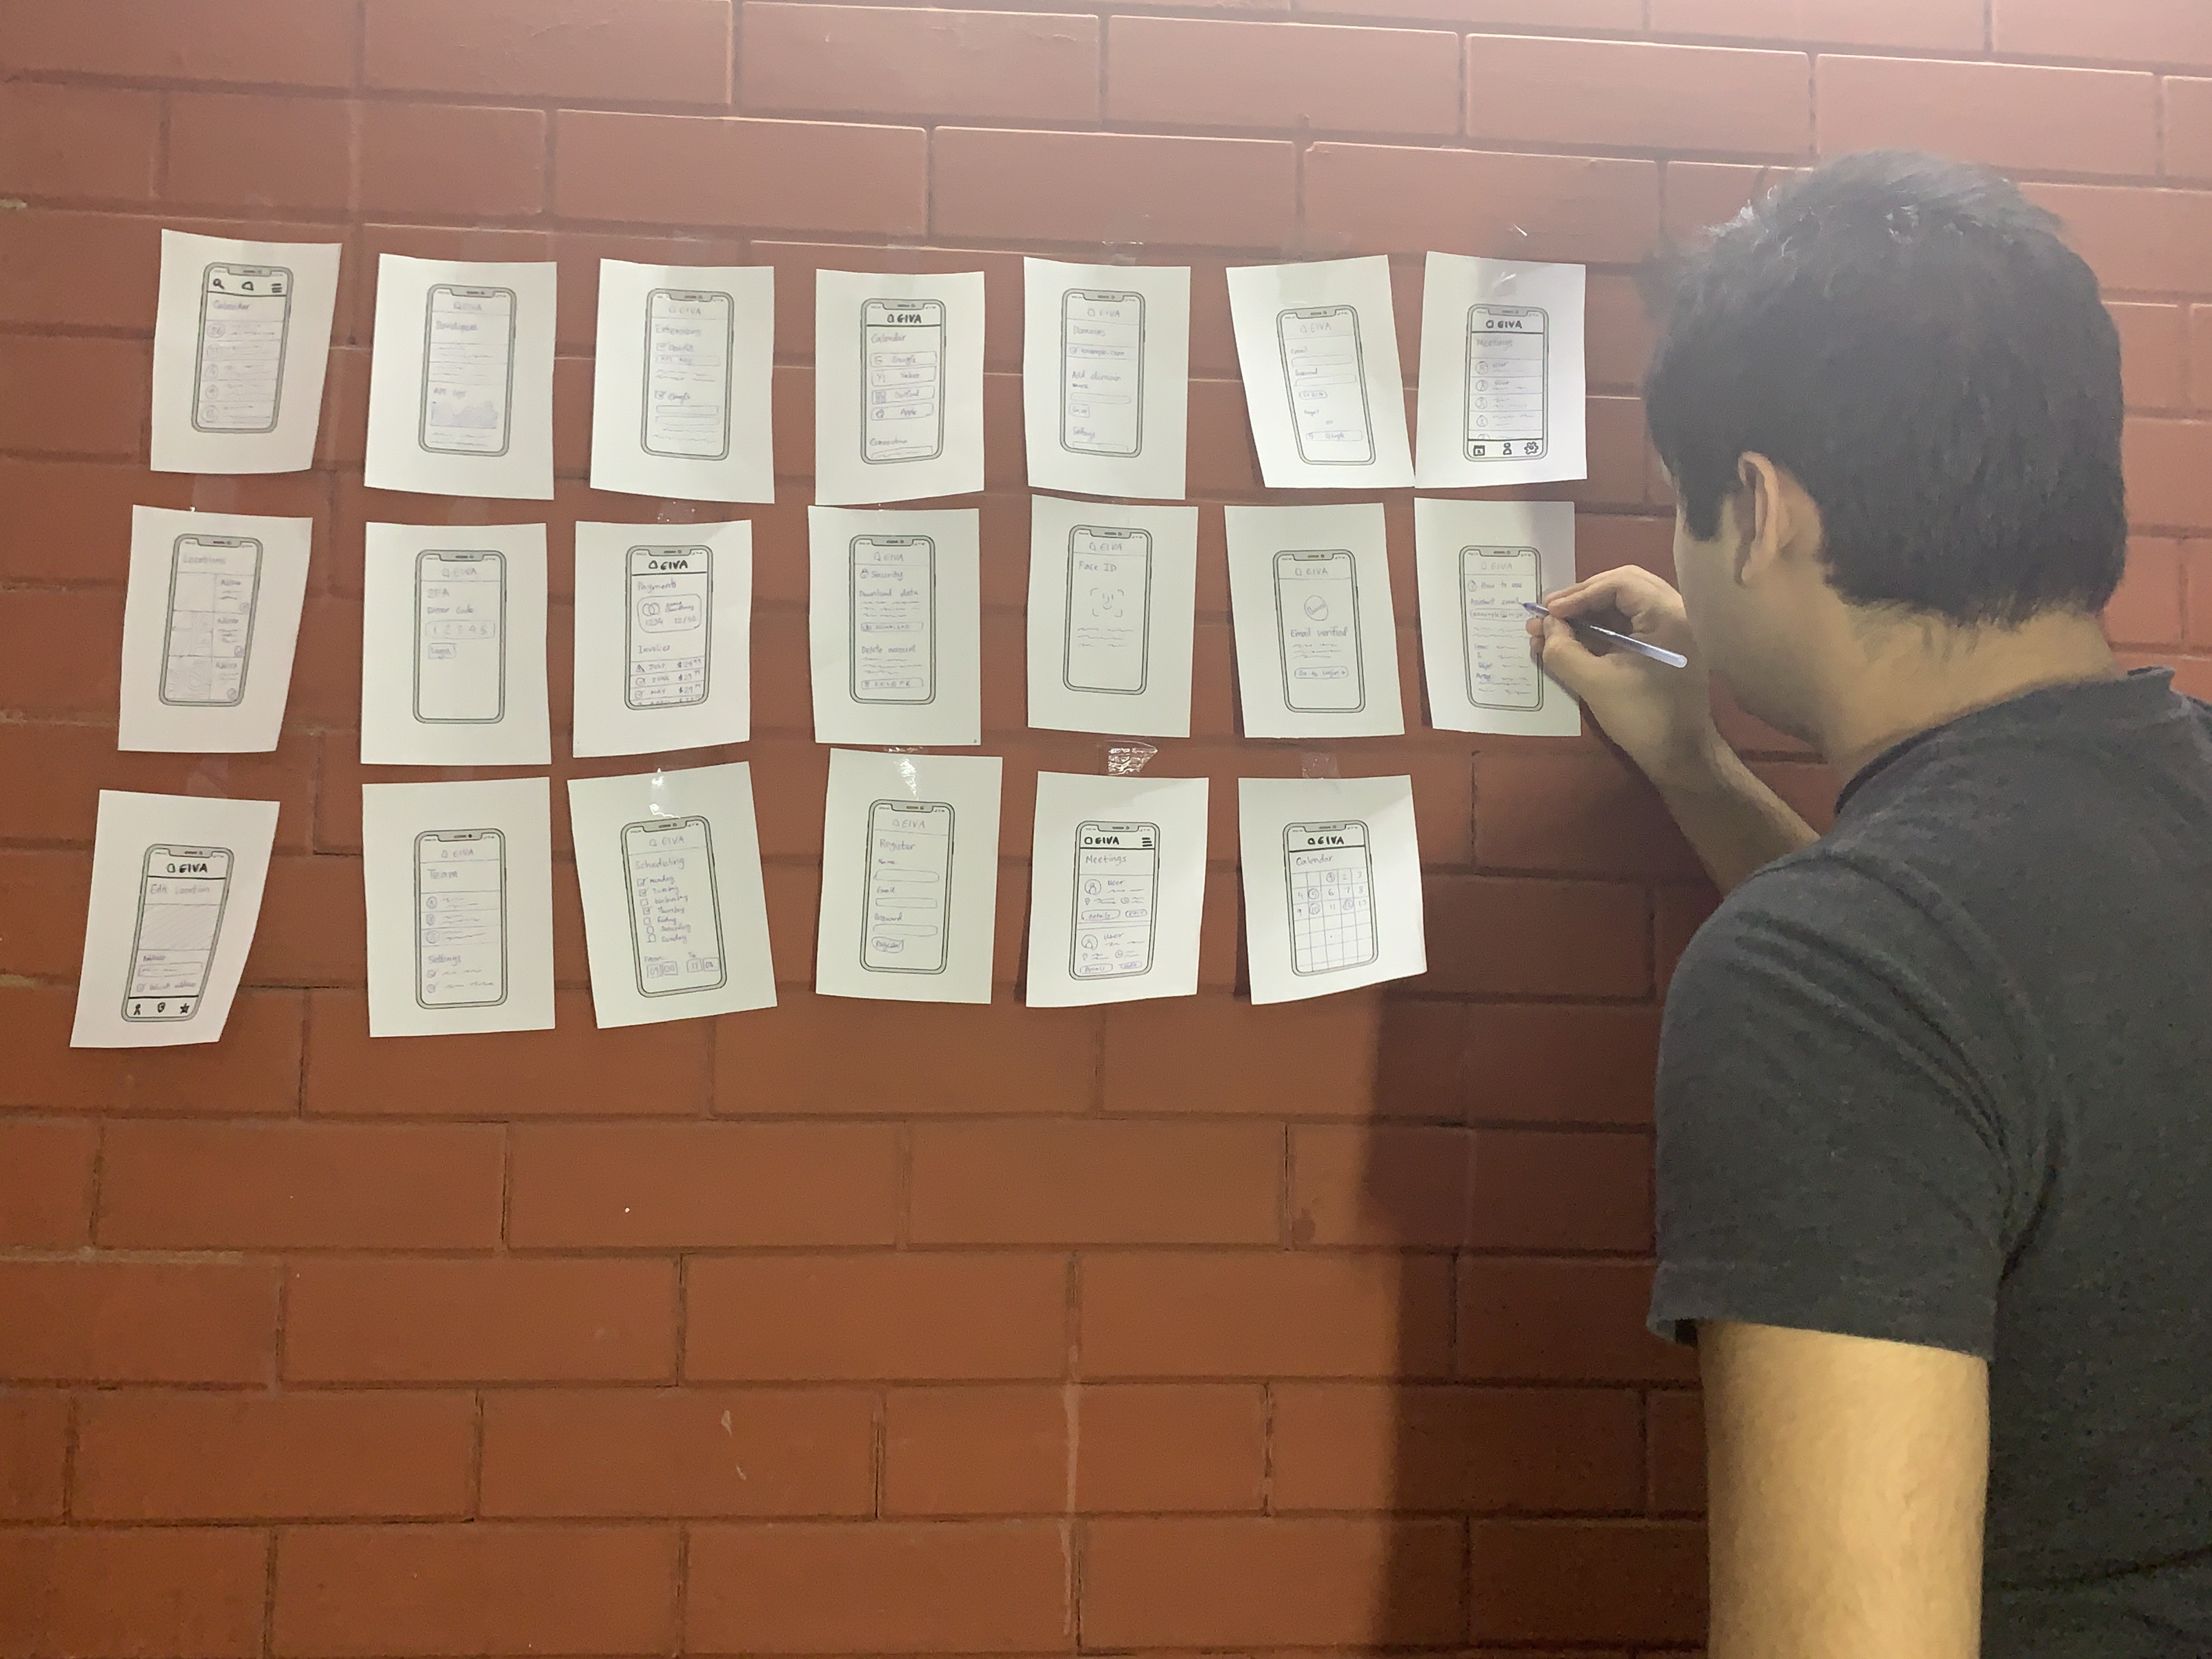
\includegraphics[scale=0.035]{ideation-wall.jpg}
	\caption{Mobile Wireframes Exploration}
\end{wrapfigure}

Lastly, both low- and high-fidelity mockups of the desktop interface were designed using Figma, a web-based vector graphics editor and prototyping tool \cite{noauthor_23-year-olds_nodate}. Figure 7 shows a comparison of a selection of these mockups. The low-fidelity mockups are used for layouting and positioning, while the high-fidelity mockups add detail such as colors, shadows, and detailed UI elements like form controls.

\vspace{15mm}

\begin{figure}[h]
	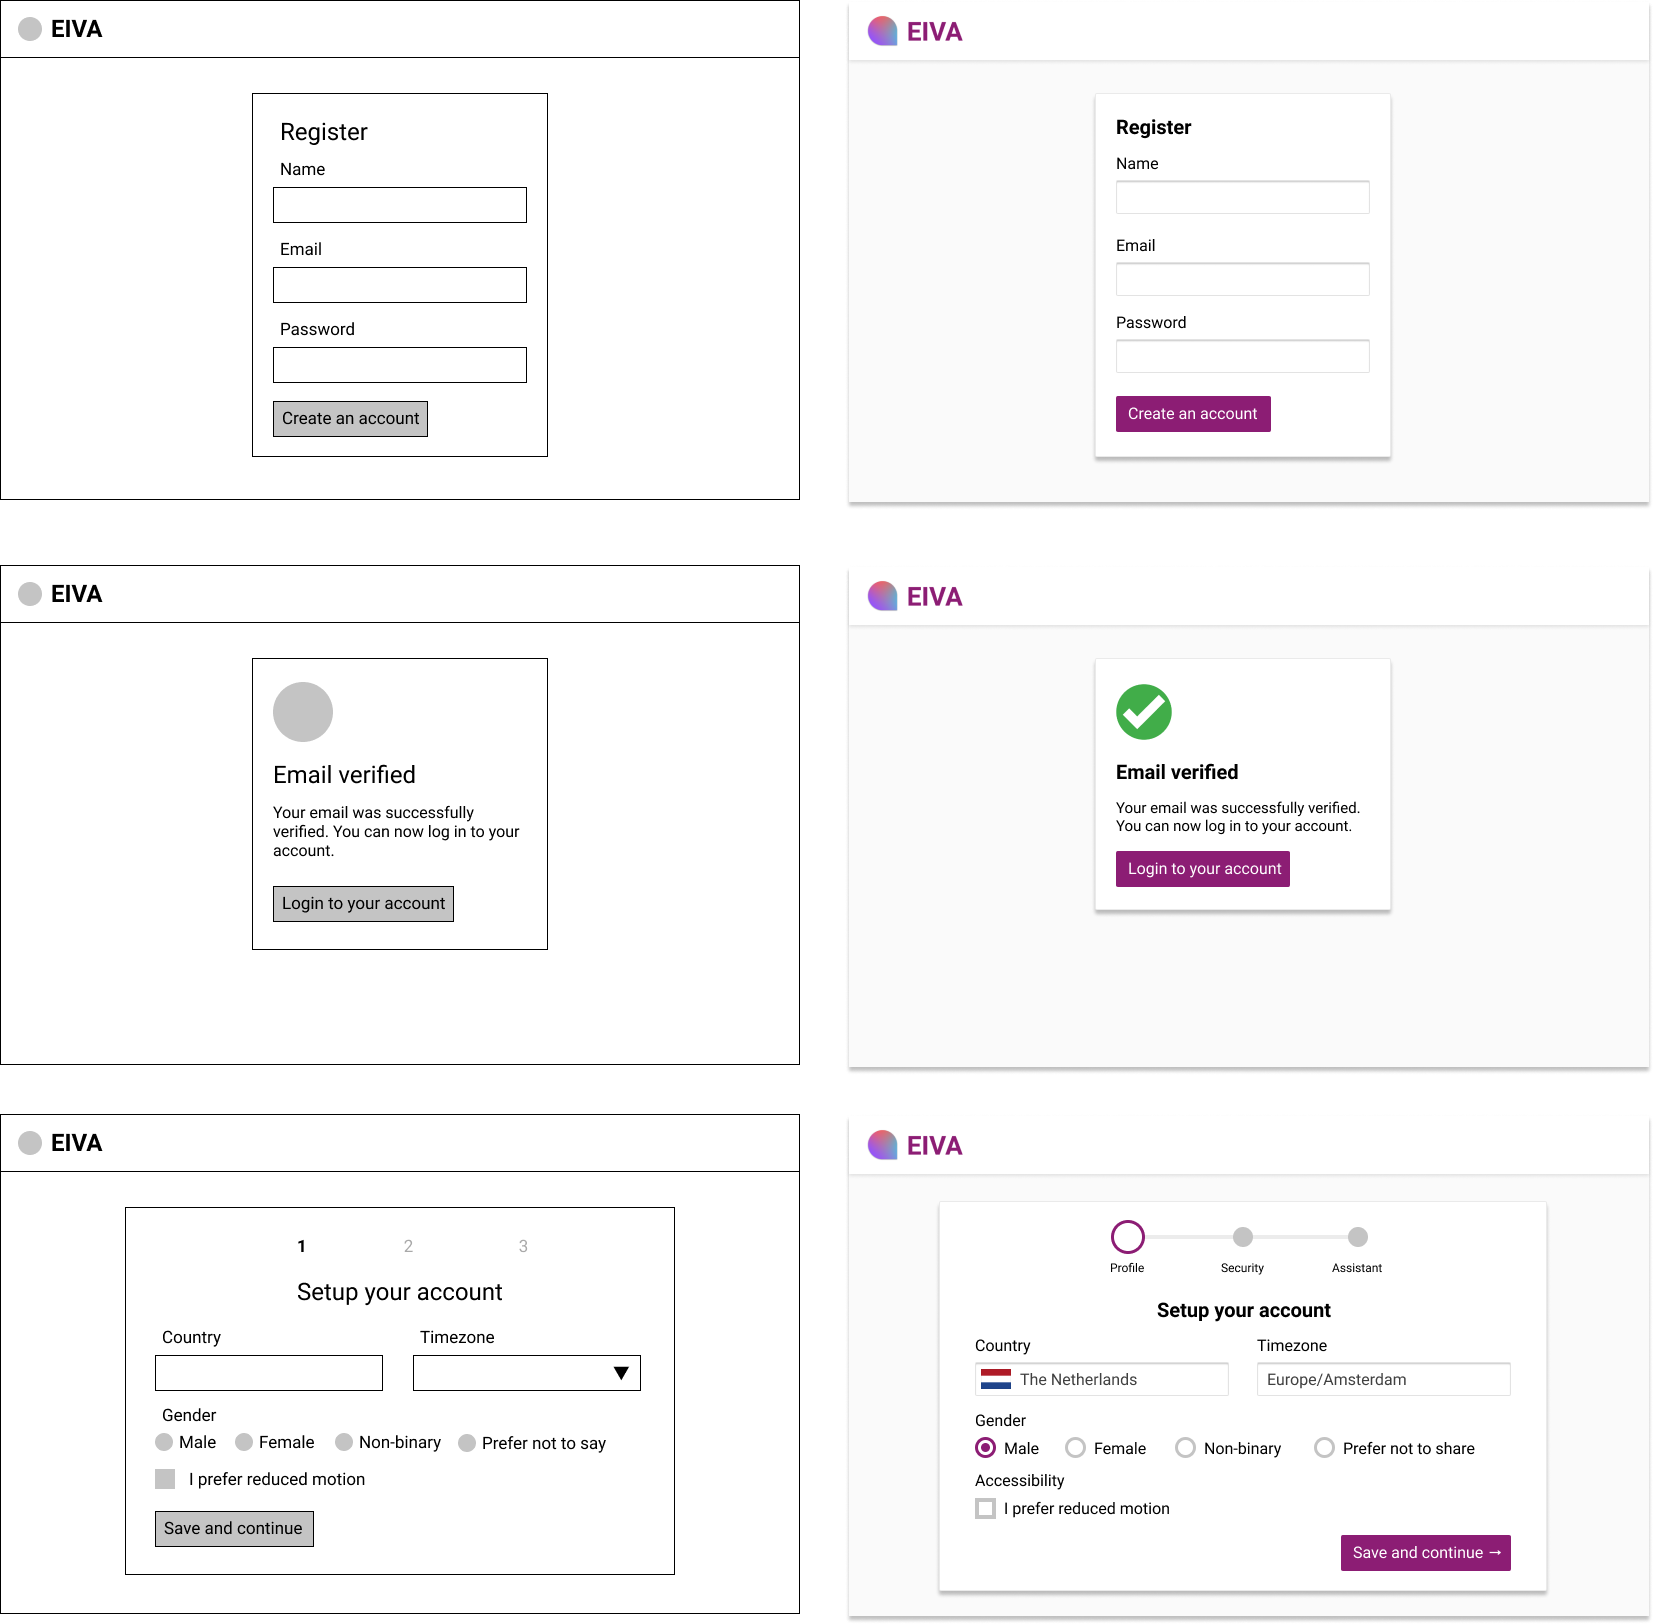
\includegraphics[width=\textwidth]{mockup-1.png}
	\caption{Comparison of low- and high-fidelity mockups}
\end{figure}

\clearpage

\section{Specification}

Based on the literature research in Section 2, this chapter focuses on specifying the key requirements for building EIVA. In the first part, the tasks required while scheduling an appointment are understood; and in the second part, personalization and customization aspects are specified.

\subsection{Tasks required in scheduling by an EIVA}

Today, most users prefer to use email for scheduling rather than currently available specialized software. A survey of workers in the field of information management found that over 80\% of the respondents use email for scheduling and organization \cite{ducheneaut_e-mail_2001}. However, this wastes a lot of time because the process of scheduling online appointments is non-trivial and requires several rounds of communication, coordination, and negotiation. This section specifies the required actions for scheduling such appointments.

\subsubsection{Understanding natural language over email}

Communication with devices using natural language is commonplace for many people today, especially with the advent of affordable smart voice assistants, such as Alexa, available on Amazon Echo; and Google Assistant, available on Google Home \cite{de_barcelos_silva_intelligent_2020}. Their interface, which translates a human's intention into a device's control commands using speech recognition and natural language interpretation, is known as a Natural Language Interface (NLI). Some NLIs are extremely useful not only because of the dialogue-style nature of interactions, but also the ability to preserve context across different queries \cite{kiseleva_predicting_2016}. Therefore, the EIVA must remember a user's preferences from previous meetings. 

Personification of the scheduling process using natural language has the additional benefit of increased likeliness of error forgiveness by end users. In a study, over 80\% of the participants who encountered errors in NLIs understanding them said that either their attitude was unaffected or the users themselves ``must have typed in something wrong" \cite{kelley_iterative_1984}. Furthermore, NLIs allow people to use their existing calendaring tools and idiosyncrasies by adopting email as the user interface and natural language conversations as the interaction mode. For example, a message such as ``Please schedule an appointment with Florian for next week" should be enough for the EIVA to take over the remainder of the process.

\subsubsection{Parameter recommendations}

Recommendation systems are frequently used in several industries to help users make better decisions. Examples of collaborative recommender systems include product recommendations on e-commerce website Amazon \cite{linden_amazon.com_2003} and TV series recommendations on the streaming provider Netflix \cite{gomez-uribe_netflix_2016}. Modern systems may use various machine learning techniques like artificial neural networks combined with feature extraction methods to find the ideal recommendation \cite{adomavicius_toward_2005}.

Scheduling a single appointment requires agreement on several parameters, such as date, time, duration, and location of meeting. Recommending a set of these parameters must be based on the user's predetermined preferences, such as the hours they prefer for scheduling calls. However, the ideal implementation of such a recommendation system may take a multidimensional approach that uses additional contextual information \cite{adomavicius_incorporating_2005}. For example, contextual information may include the user's location to account for the travel time to a recommended meeting's location; or, for international calls, it may include the guest's timezone based on their IP address.

\subsubsection{Negotiation}

Since not all guests may be available at the initially proposed time, the next major task required by the EIVA is negotiation. The negotiation mechanism allows it to be flexible about constraints imposed by the preferences of other users. Zunino and Campo (2009) note that the negotiation mechanism ``starts when two [users] do not agree on some parameter of a meeting," such as the date, time, or location of the meeting \cite{zunino_chronos:_2009}. Then, the guest may propose a new set of parameters for the meeting, for example by modifying its time. The EIVA will evaluate whether the proposal is convenient or not by comparing the ``likeliness of reaching a consensus using the previous meeting parameters with the proposed parameters." In this step, it can also make a judgement call by choosing to ignore part of the user's preferred parameters in order to agree with the guests. This back-and-forth negotiation process needs to occur asynchronously, ``sometimes requiring several days for the parties to reach consensus" \cite{cranshaw_calendar.help:_2017}.

\subsubsection{Renegotiation and confirmation invitations}

In the dynamic environment that is the modern workplace, changing appointment parameters is commonplace. A study found that 66\% of all scheduled meetings by a CEO underwent a parameter change \cite{dennis_how_2018}. Inevitably, once a meeting is scheduled, it requires ``continuous maintenance, as new events often prompt meeting updates and reschedules" \cite{cranshaw_calendar.help:_2017}. To finalize the meeting parameters, the EIVA should take into account the parameter preferences of both the user and all guests.

To make sure that all guests have the most recent parameters, confirmations and reminders may be sent by the EIVA. However, not all users use the same calendaring software, with some professionals using no digital calendar at all. Kincaid (1985) reported that approximately one half of all meetings scheduled by professionals were with users using a different calendaring system than their own \cite{kincaid_electronic_1985}. Therefore, the EIVA will be required to send these emails using industry standards supported by most software. The primary standard to store and exchange calendaring and scheduling information is the Internet Calendaring and Scheduling Core Object Specification (iCalendar) \cite{desruisseaux_internet_2009}.

\subsection{User Configuration}

\subsubsection{Authorship}

One of the first discussed questions with the client is whether or not recipients should clearly know that an email sent by EIVA is not actually sent by a human assistant. This question of authorship is not just a technical one, but an ethical one as well. In journalism, for example, there are articles entirely written by AI-powered virtual agents, which raises the question \emph{Who is the author of an article written by a virtual agent?} A 2005 study found that research participants attribute story credit to the programmers who developed the AI or the news organization publishing the story \cite{montal_i_2017}.

The key reason why authorship is important is credibility. If you know the name of the author of an article in a major newspaper or magazine, you can find out more information about them, perhaps by visiting their social media handles. If you have any questions about their work, or found a mistake in their article, you can contact them directly. In the case of an article written by an unnamed virtual agent, the only option is to find the contact information of the publication. This is also the case with EIVA, where users can name their own assistant and essentially create a human-like entity, but without the necessary digital history required for authenticity.

\paragraph{Authorship Clarity}

In news articles written by virtual agents, there is ``no visible indicator for readers to verify whether an article was written by a robot or human", which raises issues of transparency \cite{dorr_ethical_2017}. In the case of EIVA, if an AI assistant is impersonating a human assistant to send emails on the professional's behalf, it raises the same ethical question of whether the end user receiving the email should know that it was not written by a human. Some users may be completely fine with deceiving recipients on such a ``trivial" authorship question, while for others this sets a powerful and potentially harmful precedent for AI authorship and will choose to make that information clear.

Therefore, it is recommended to keep such decisions customizable. Using the EIVA website's settings page, consumers should be able to set preferences about whether they want their assistant to inform end users about the fact that they are virtual agents, not human assistants. By default, this is preselected for all users, and is a simple checkbox user interface with the message ``Inform recipients that your assistant is a virtual assistant". This clarity highlights the commitment to personalization that such a product should bring.

\subsubsection{Sensible Defaults}

The previous section sheds light on the importance of defaults, such as letting recipients know about the AI nature of the assistant by default. Using the feedback from users, especially for customizable options related to individual privacy, the less secure and more open options should always be opt-in, not opt-out, to ensure sensible rather than opinionated defaults. Other configuration options can be based on the results of the initial survey with users and feedback from stakeholders.

It has been estimated that 95\% of all users stick to the default settings in an application, and don't bother to change them \cite{catalanotto_95_2019}. Therefore, this is an important responsibility on the hands of designers and engineers to ensure that the default options are most secure. In EIVA, options such as email tracking, directly connecting a calendar, or even sharing personal video meeting links, are all optional and opt-in, so the default state is always most secure.

\subsubsection{Privacy-first}

The privacy precedent that most virtual assistants have set is not highly positive. Personal assistants in the form of smart speakers like Amazon Echo (running Alexa) and Google Home (running Assistant) have ``begun to significantly alter people’s everyday experiences with technology" \cite{pridmore_personal_2020}. These virtual assistants can continually improve with increased usage using deep learning \cite{kepuska_next-generation_2018}. Although this makes the assistants more useful over time, they also ``amplify the overall debate about privacy issues" \cite{zeng_end_2017}.

For example, an Echo device unintentionally recorded a Portland family's private conversations and shared it with a random person from their contact list \cite{noauthor_this_nodate-1}. For EIVA, the learning is simple: make sure no personal information is recorded if it is not strictly necessary, and users should be able to configure what they want to share.

\subsubsection{Gender Bias}

There is often visible gender bias when it comes to personal assistants or secretaries \cite{noauthor_why_2018}. Historically, these were executive assistants, but modern technologies have translated these biases to virtual assistants as well. When asked about why Cortana is female, a \emph{Microsoft} spokesperson said Cortana can technically be genderless, but the company did immerse itself in gender research when choosing a voice and weighed the benefits of a male and female voice \cite{pcmag_real_2018}, ``for our objectives — building a helpful, supportive, trustworthy assistant — a female voice was the stronger choice".

Apple's Siri and Google Assistant offer the option of changing the voice to male, but Alexa and Cortana don't have male counterparts. The first United Nations' examination of gendering of AI technology found that ``gender imbalances in the digital sector can be `hard-coded' into technology products" \cite{noauthor_id_nodate}. In that report, the following problems are highlighted:

\begin{itemize}
	\item Digital assistants reflect, reinforce and spread gender bias
	\item They model acceptance and tolerance of sexual harassment and verbal abuse
	\item They send explicit and implicit messages about how women and girls should respond to requests and express themselves
	\item They make women the ‘face’ of glitches and errors that result from the limitations of hardware and software designed predominately by men
	\item They force synthetic ‘female’ voices and personality to defer questions and commands to higher (and often male) authorities
\end{itemize}

The UN report makes 15 recommendations, including ``[ending] the practice of making digital assistants female by default." For EIVA, this is an important lesson because with the intention of sounding friendly, the original name for EIVA was \emph{Ara}. However, the gender role that accompanies this is a big problem, therefore the name was changed to EIVA, which is an acronym for Email-based Intelligent Virtual Assistant, and yet sounds friendly and human-like.

However, though the name of the service is EIVA, as discussed in the previous section, customizability is a key part of the user experience, and users should be able to pick custom names for their assistants via the interface. Unisex names like \emph{Alex} and \emph{Jesse} can be used by end users; the idea is to make the assistant completely customizable. To make this easy, the first setting in the user interface is to select the assistant's name and signature, which users can freely pick.

\newpage

\section{Realization}

EIVA consists of a frontend web app that users directly interact with, and a backend API that powers it.

\subsection{Backend APIs}

EIVA's backend project is based on Staart API, an open source framework to build Software as a Service (SaaS) products with TypeScript. With Staart API, several features that typical web apps require, such as user management, organizations, authentication, API gateway, etc., are built-in and do not require significant effort for setup. Staart API is also built by the author of this graduation project and has over 200 stars on GitHub.

\subsubsection{Configuration Management}

Using ES Modules, the ECMAScript standard for working with modules, data and structure types can be imported and exported \cite{noauthor_es_nodate}. The \texttt{src/config.ts} file acts as the central configuration manager and sets default values for keys not available in the environment.

The Twelve-Factor App methodology recommends storing configuration in the environment, separate from the code, and \texttt{dotenv} is used to read environment variables from a \texttt{.env} file \cite{noauthor_twelve-factor_nodate}. This library makes values available in \texttt{process.env}, Node.js's object to access environment variables.

For example, the \texttt{PORT} constant defines the port the app should listen on, and defaults to port 80:

\begin{alltt}
\textcolor{keyword}{import} \{ config \} \textcolor{keyword}{from} \textcolor{string}{"dotenv"};
\textcolor{variable}{config}();
\textcolor{keyword}{export const} \textcolor{symbol}{PORT} = process.\textcolor{variable}{env}.\textcolor{symbol}{PORT} ? parseInt(process.\textcolor{variable}{env}.\textcolor{symbol}{PORT}) : \textcolor{literal}{80};
\end{alltt}

Then, when initializing the app, this value is imported:

\begin{alltt}
\textcolor{keyword}{import} \{ PORT \} \textcolor{keyword}{from} \textcolor{string}{"./constants"};
\textcolor{keyword}{import} \{ Server \} \textcolor{keyword}{from} \textcolor{string}{"@staart/server"};
\textcolor{keyword}{export class} Staart \textcolor{keyword}{extends} Server \{
  \textcolor{keyword}{public} start(port: number = \textcolor{symbol}{PORT}): \textcolor{keyword}{void} \{
    this.\textcolor{variable}{app}.\textcolor{variable}{listen}(port, () => console.\textcolor{variable}{log}(\textcolor{string}{`Listening on} \$\{port\}\textcolor{string}{`}));
  \}
\}
\end{alltt}

This central management makes it very easy to update defaults (like port 80), and the \texttt{.env} file contains environment-specific values, like port 7000 for development and 443 for production. A \texttt{.env.example} file is available in the repository for reproduction. A total of 68 exported members configure various parts of the application, from database connection URLs to secret keys for signing JSON Web Tokens (Section 6.1.7).

\subsubsection{Natural Language Processing}

There are three Natural Language Processing (NLP) systems implemented in EIVA's backend --- language detection and variable extraction, intent classification, and date parsing. These systems work together during the scheduling process (Section 6.1.11) and use various libraries.

\paragraph{Language Detection and Variable Extraction}

To identify the language of an incoming email, Google Cloud's Natural Language API is used. This provides both the language and list of entities found, such us names of people and places. Using this API is free of cost for up to 5,000 requests every month, which is more than enough for this project, since this API is only used to identify the language to ensure the response of the email is also in the correct language.

\paragraph{Intent Classification}

A Naive Bayes classifier is used to identify the intent of an incoming email from one of four categories --- setting up a new appointment, rescheduling an existing appointment, canceling an appointment, or sending a summary of the appointments for the day.

Naive Bayes classifiers are probabilistic classifiers, meaning that they calculate a probability distribution over a set of classes, are are based on applying Bayes' theorem with strong independence assumptions between the features. Features are independent if the realization of one does not affect the probability distribution of the other; for example, a fruit can be considered an apple if it is round and red, and the naive Bayes classifier considers each of these features to contribute independently to the probability that this fruit is an apple, regardless of any possible correlations between the color or roundness \cite{noauthor_lecture_nodate}.

The \texttt{BayesClassifier} class of Natural, a general natural language facility for Node.js, is used for the naive Bayes classification. Training data consisting of common phrases to perform the aforementioned actions is used, for example:

\begin{alltt}
\textcolor{keyword}{import} \{ BayesClassifier \} \textcolor{keyword}{from} \textcolor{string}{"natural"};
\textcolor{keyword}{const} classifier = new \textcolor{variable}{BayesClassifier}();

classifier.\textcolor{variable}{addDocument}(
  [
    \textcolor{string}{"set up an appointment"},
    \textcolor{string}{"schedule a call"},
    \textcolor{string}{"meet me for dinner"},
  ],
  \textcolor{string}{"setupNewAppointment"}
);
classifier.\textcolor{variable}{addDocument}(
  [
    \textcolor{string}{"i can't make it"},
    \textcolor{string}{"reschedule this call"},
    \textcolor{string}{"find another time"},
  ],
  \textcolor{string}{"rescheduleAppointment"}
);

classifier.\textcolor{variable}{train}();
\end{alltt}

In the above example, when the classifier receives a new string, such as ``I don't think I'll be able to make it to this time", it will return a higher probability for \texttt{rescheduleAppointment} than \texttt{setupNewAppointment}, as the following example shows:

\begin{alltt}
classifier.\textcolor{variable}{getClassifications}(
  \textcolor{string}{"i don't think I'll be able to make it to this time"}
);
\end{alltt}

Here, the value of rescheduling is 0.333... and that of setting up a new appointment is 0.1666..., which shows that the naive Bayes classifier works at a decent accuracy, even with an extremely small training dataset. In EIVA, the training dataset is larger and there are four categories of classifications.

\paragraph{Date Parsing}

Lastly, Chrono, a date parsing library, is used to understand natural language dates and times. Chrono can understand specific days like ``today" and ``tomorrow", relative dates and times like ``this Friday at 13:00" and ``two weeks from now", and absolute values like "Aug 17, 2020".

In the Netherlands, a convention is to write times in 24-hour format with a period as the hour-minute separator (e.g., 14.30 instead of 2:30 pm) \cite{noauthor_8h30_nodate}. Since Chrono is not optimized for understanding this format, a regular expression (regex)-based replacement from period to colon is done on the entire text string before parsing. Other special cases, such as no separator, are also handled.

\subsubsection{Transactional Emails}

EIVA does not send any promotional emails, only transactional emails for authentication-related cases like email verification and password reset links, and communication to the guests or host from the assistant \cite{noauthor_everything_2018}.

Email templates are defined in Markdown, and rendered with variables using Mustache. Markdown is a lightweight markup language with plain-text-formatting syntax created by John Gruber with Aaron Swartz, and was selected because of its ease of conversion to both HTML and plain text \cite{noauthor_daring_nodate}. Since there are also several variables that need to be replaced in the template, Mustache, a web template system is used alongside Markdown.

The author's \texttt{@staart/mustache-markdown} package makes rendering easy by exposing a single interface for both Mustache and Markdown \cite{noauthor_staart/mustache-markdown_nodate}. For example, an email verification email template may contain:

\begin{alltt}
Hello, \textcolor{variable}{\{\{name\}\}}! Please click on this link to verify your email:
![\textcolor{variable}{\{\{link\}\}}](Verify my email).
\end{alltt}

When an object containing data is provided (say, the name `Florian' and an example link), the following HTML is generated:

\begin{alltt}
\textcolor{variable}{<p>}Hello, Florian! Please click on this link to verify your email:
\textcolor{variable}{<a href=}\textcolor{string}{"https://example.com"}\textcolor{variable}{>}Verify my email\textcolor{variable}{</a>}.\textcolor{variable}{</p>}
\end{alltt}

Emails are sent using Amazon Web Services' Simple Email Service (SES) using Nodemailer, a library that provides a simple API to send email using Node.js and supports both SES and SMTP \cite{noauthor_nodemailer_nodate}. Each email is sent with both the plain text and HTML versions, with DKIM and SPF verification.

For ``magic links" for email verification, password reset, or appointment confirmation, JSON Web Tokens (JWT) are used. JTWs are URL-safe and have encrypted data, and can be verified server-side without additional database queries. A queue is used to send emails sequentially, implemented using Redis (Section 6.1.7). This ensures that the rate limits imposed by SES are respected, and that undelivered emails can be sent again (up to 3 tries).

\subsubsection{Authentication}

Users can create an account using the web app by entering their name, email, and password. Passwords are hashed using \texttt{bcrypt} before storage, which introduces a work factor and is therefore much safer than general-purpose hash functions \cite{provos_future-adaptive_1999}. It also has built-in salting to prevent rainbow table attacks \cite{noauthor_how_2010}.

For authentication, the industry-standard access/refresh token combination is used. When logging in, both tokens are generated and stored on the client (Section 6.2.3), with the access token expiring after 15 minutes and the refresh token after 30 days. The expired access token can be exchanged for a new one using the refresh token.

Both tokens are JWTs and contain all required information; the access token includes details about the user (such as their name and role) whereas the refresh token only includes the user ID. Furthermore, the web app also allows users to see a list of their logged in sessions and invalidate refresh tokens, which are then blacklisted in Redis (Section 6.1.7).

\begin{figure}[h]
	\centering
	\begin{minipage}{.47\textwidth}
		\centering
		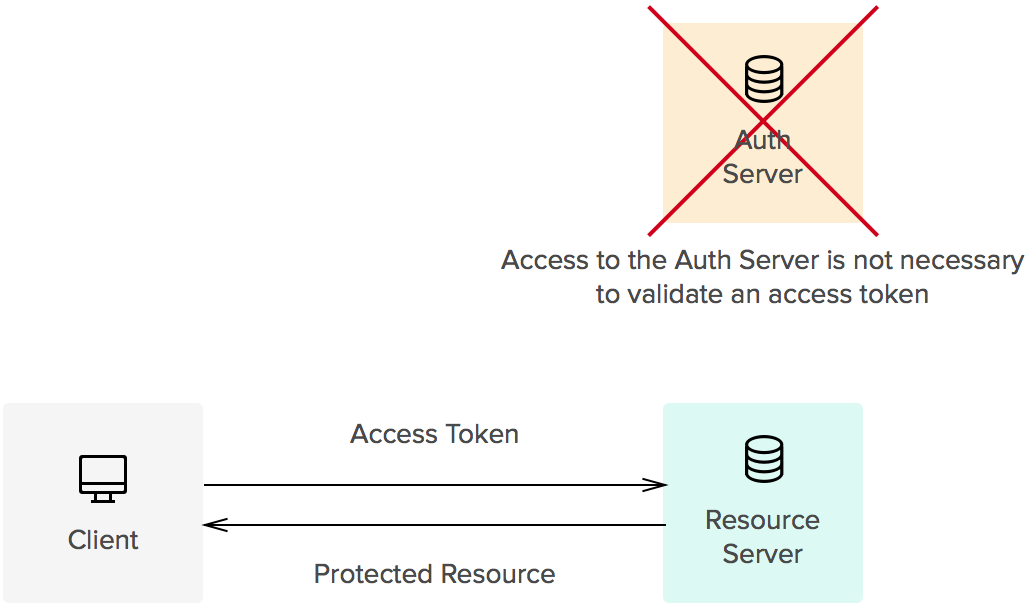
\includegraphics[width=5.75cm]{access-token.png}
		\captionof{figure}{Access Token Process \cite{noauthor_refresh_nodate-1}}
	\end{minipage}%
	\hspace{.5cm}
	\begin{minipage}{.47\textwidth}
		\centering
		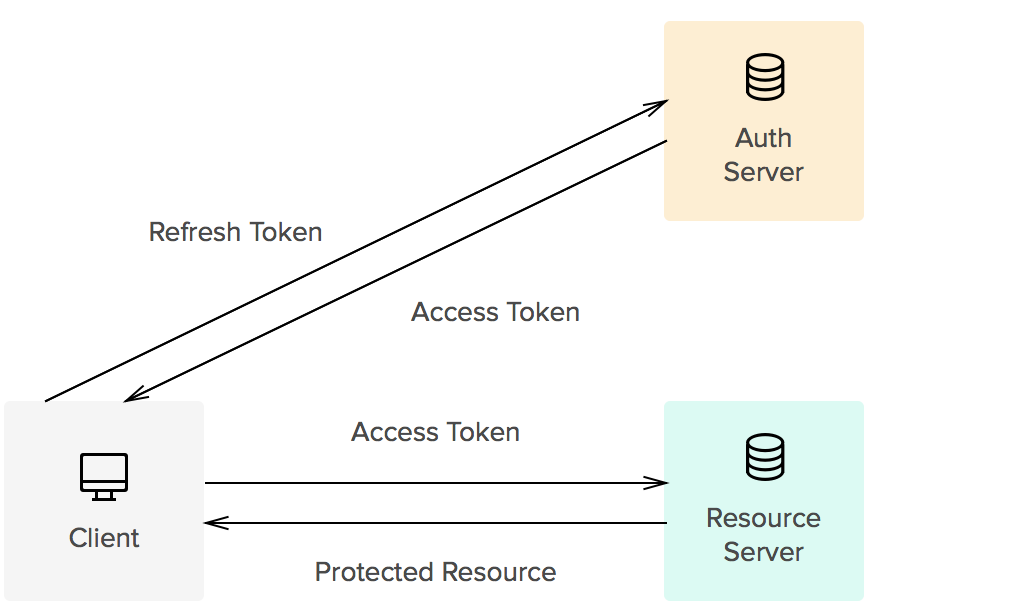
\includegraphics[width=5.75cm]{refresh-token.png}
		\captionof{figure}{Refresh Token Process \cite{noauthor_refresh_nodate-1}}
	\end{minipage}
\end{figure}

Since many professionals prefer using multiple emails (perhaps a personal and a work email) and the assistant should recognize all their emails, a user account can be associated with multiple emails. This also means that users are free to log in with any of their verified emails.

\paragraph{Rate Limits}

Rate limits are used to control the rate of requests to the API and is also used to prevent DDoS attacks \cite{noauthor_rate_nodate}. An HTTP 429 (Too Many Requests) error is thrown if a client makes too many requests within a given time frame. By default, 60 requests per minute are permitted per IP address.

For programatic access to the service, users can generate API keys or access token to control their assistant or accounts respectively. The frontend web app also uses such an API key for an increased rate limit of 1,000 requests per minute. An in-memory key-value store is used to track these limits.

Lastly, brute force and speed limits are also imposed. To prevent brute force attacks on authentication endpoints like login and register, more than 5 requests in a period of 5 minutes results in a delay of 250 milliseconds per request. Similarly, all other endpoints also add a 100 millisecond per request delay after 1,000 requests within ten minutes.

\subsubsection{Database and Storage}

MariaDB is used as the primary database management system for the backend. MariaDB is a drop-in replacement for and a community-developed fork of MySQL, intended to remain free and open source software under the GNU General Public License \cite{noauthor_mariadb/server_2020}. For communication with the database, the open source database toolkit \emph{Prisma} is used. Prisma replaces object-relational mapping with a query builder and TypeScript schema generator. It also allows for database migrations and versioned schema stored in the repository \cite{noauthor_prisma/prisma_2020}.

Relations are used extensively in the database; for example, the \texttt{users} table has a reference to nearly all other tables. Figure 10 visualizes a simplified version of the database schema, and Appendix 5 contains the entire schema.

\begin{figure}[h]
	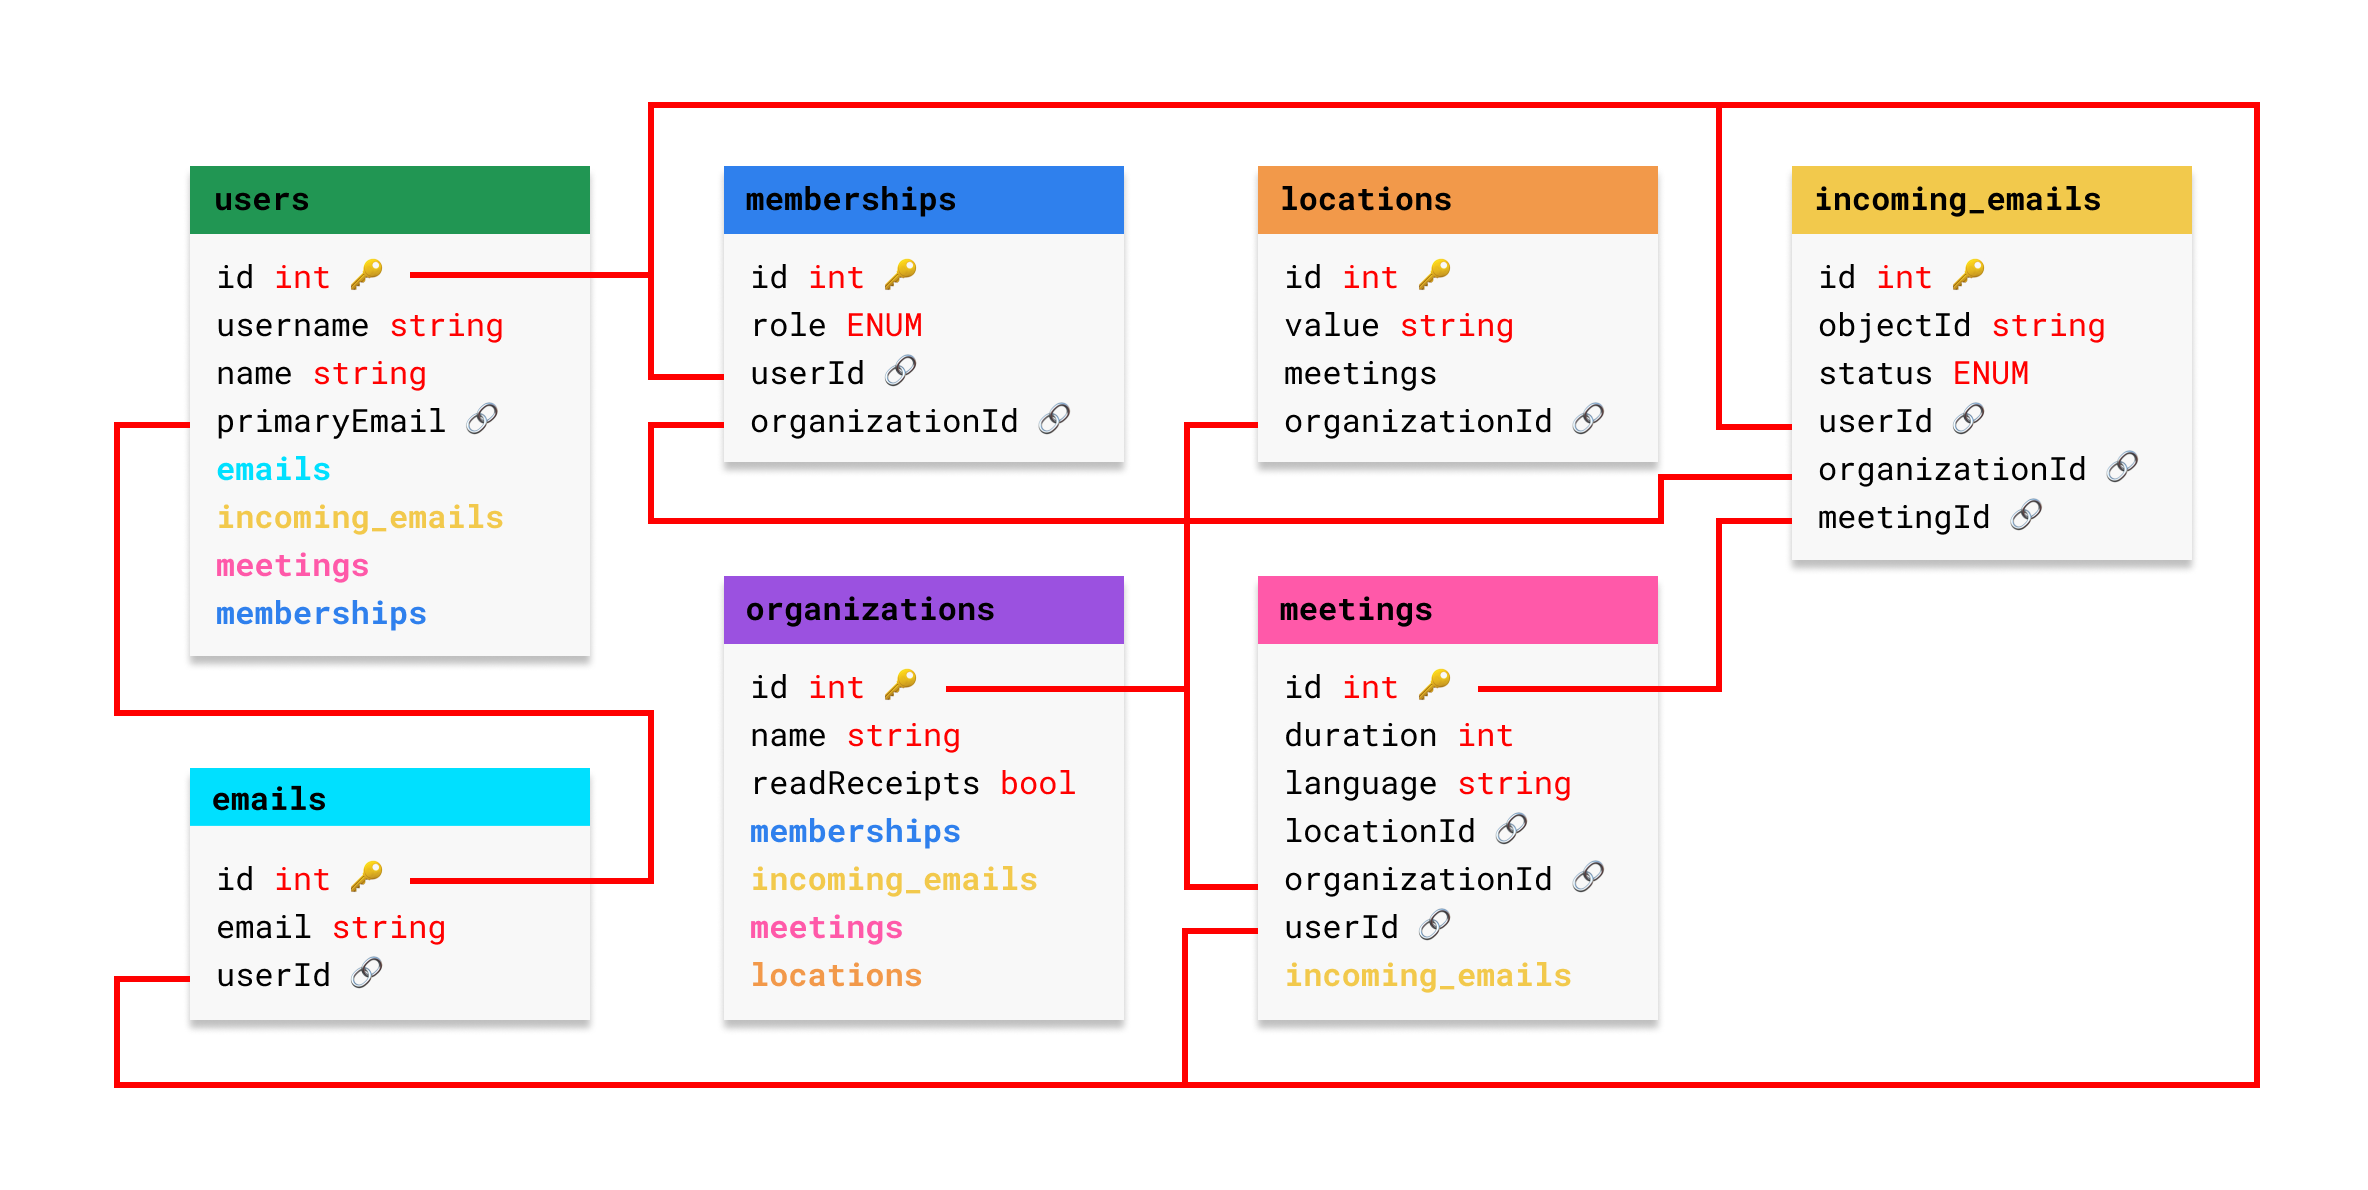
\includegraphics[width=\textwidth]{database-basic.png}
	\caption{Simplified Database Schema with Relations}
\end{figure}

\paragraph{Redis}

Apart from MariaDB, \emph{Redis} is used for storing data that requires minimal query latency. Redis is an in-memory key–value database, and in-memory processing has been called ``the ultimate solution to latency" \cite{alami_supply_2018}. For workflows such as checking if a JWT has been invalidated, a MariaDB database query takes hundreds of milliseconds, whereas Redis only takes tens, and is therefore used for caching and invalidation in EIVA.

Redis is also used as a message queue using Redis Simple Message Queue (RSMQ) which implements a queue with guaranteed message delivery to one recipient. This is used to queue outbound webhooks and emails, which are sequentially sent every minute using a scheduled job (Section 6.1.7).

\paragraph{ElasticSearch}

ElasticSearch, a Lucene-based search engine, is used for storing server logs and analytics data \cite{noauthor_elastic_nodate}. ElasticSearch is open source and capable of full-text search, which makes it extremely useful to sort through thousands of usage events \cite{noauthor_elastic/elasticsearch_2020}. Amazon Web Services (AWS) offers Open Distro for ElasticSearch with increased security features, including data encryption at rest and Kibana authentication \cite{noauthor_open_nodate}, which is used for this project. In Section 7.2, data stored in this ElasticSearch instance is computed and analyzed.

\paragraph{AWS S3}

Although there are no binary files, the API still deals with large text files like raw incoming emails, typically between 1 and 10 kilobytes in size. A database is not ideal for storing such documents, so AWS's Simple Storage Service (S3) is used. S3 provides object storage along with backup, recovery, and encryption, and provides a Node.js API wrapper to easily upload and fetch files.

\subsubsection{API Endpoints}

The backend API endpoints are versioned with a \texttt{/v1} prefix and categorized, for example the login endpoint is \texttt{POST /v1/auth/login}.  Since there are tens of total endpoints, it's useful to categorize them for development and management, and each API category is defined in Table 3. Each endpoint category prefix is automatically generated from the \texttt{controllers} directory in Staart API's build process, based on the subdirectory it is located in. For example, the user emails controller file \texttt{controllers/users/\_id/emails.ts} generates the endpoint \texttt{/v1/users/:id/emails} where \texttt{:id} is a user ID.

\begin{table}[!htb]
	\begin{minipage}{1\linewidth}
		\caption{API Prefixes}
		\centering
		\begin{tabular}{lll}
			\hline
			\textbf{Prefix} & \textbf{Description} \\
			\hline
			\texttt{/admin} & Administration and analytics \\
			\texttt{/api} & Public API \\
			\texttt{/auth} & Authentication \\
			\texttt{/organizations} & Teams and assistant settings \\
			\texttt{/users} & User settings \\
			\texttt{/webhooks} & Incoming webhooks \\
			\hline
		\end{tabular}
	\end{minipage}%
\end{table}

\paragraph{Public API}

The internal process that EIVA uses to schedule appointments (Section 6.1.9) has also been designed in a way to be consumable by other clients. A public API has been developed for each action as listed in Table 4.

\begin{table}[!htb]
	\begin{minipage}{1\linewidth}
		\caption{Scheduling API Endpoints}
		\centering
		\begin{tabular}{lll}
			\hline
			\textbf{Method} & \textbf{Endpoint} & \textbf{Description} \\
			\hline
			\texttt{POST} & \texttt{/classify} & Classify text using NLP \\
			\texttt{POST} & \texttt{/parse-email} & Parse a raw email \\
			\texttt{POST} & \texttt{/smart-tokenize} & Intelligently tokenize text \\
			\texttt{POST} & \texttt{/parse-email} & Parse a raw email \\
			\hline
		\end{tabular}
	\end{minipage}%
\end{table}

Developers can use these endpoints in the future to intelligently understand incoming emails and build other applications on top of the EIVA platform.

\subsubsection{Scheduled Jobs}

To automate common tasks, specific jobs are scheduled using \texttt{cron}, a Node.js API for the time-based job scheduler of the same name. For example, new data is fetched from message queues every minute to send outbound emails, trigger outbound webhooks, and store logs in ElasticSearch.

\begin{table}[!htb]
	\begin{minipage}{1\linewidth}
		\caption{Scheduled Jobs}
		\centering
		\begin{tabular}{lll}
			\hline
			\textbf{Expression} & \textbf{Repetition} & \textbf{Job} \\
			\hline
			\texttt{0 0 * * *} & Every day & Delete old server logs \\
			\texttt{0 * * * *} & Every hour & Delete expired sessions \\
			\texttt{0 * * * *} & Every hour & Update errored emails \\
			\texttt{* * * * *} & Every minute & Get new data from message queues \\
			\hline
		\end{tabular}
	\end{minipage}%
\end{table}

\subsubsection{Third-party APIs}

Other third-party APIs are used for specific utilities, such as \emph{Clearbit} to fetch details about a person from their email address. Clearbit's Enrichment API uses over 250 public and private sources and provides several datapoints, such as name, professional, company, and timezone. This is used to better understand the context of guests in meetings. Other APIs used in EIVA include \emph{Stripe} to accept end-user payments \cite{wittern_web_2018}.

\subsubsection{Scheduling Process}

To schedule a new appointment, users have to send an email to their guests with their assistant in CC. Every assistant has an auto-generated but customizable \texttt{@myeiva.com} email address that is shown on the \emph{How to Use} page (Section 6.2.4). Figure 11 shows that every time a new email is received by AWS SES, the raw email is stored in AWS S3 and a Lambda serverless function is triggered, which is turn triggers an API webhook. The API webhook is triggered with an HMAC-SHA256 token consisting of the object ID of the S3 email signed with a shared secret to ensure that the webhook is not publicly usable.

\begin{figure}[h]
	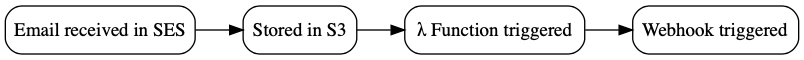
\includegraphics[width=\textwidth]{ses-process.png}
	\caption{Email Received to Webhook Process}
\end{figure}

When the webhook is triggered, the API starts with trying to understand the incoming email. Figure 12 graphs the process from trigger to classification, consisting of fetching the raw email from AWS S3, parsing the raw email, finding the team and user based on the assistant email, setting up the database record, and tokenizing and classifying the email contents.

\begin{figure}[h]
	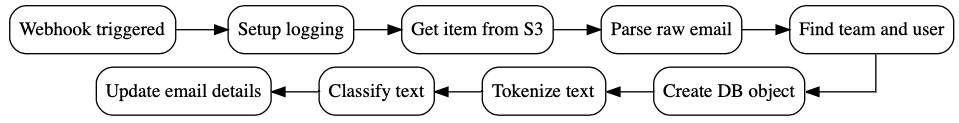
\includegraphics[width=\textwidth]{webhook-process.png}
	\caption{Webhook to Classification Process}
\end{figure}

\begin{figure}[h]
	\center
	
\includegraphics[width=7cm]{schedule-process.png}
	\caption{Scheduling Process}
\end{figure}

After the email is classified as requesting a new appointment, the process described in Figure 13 is triggered to schedule a new appointment for the user and their guests. First, the entire email text is modified for consistent date formats; then, a Google API is used to detect the language of the email (Dutch or English); then, all the guests are detected, and Clearbit is used to find additional information about them, if enabled. Then, dates and times are found using Chrono (Section 6.1.2), and 3 time slots are recommended along with the location and an email is sent. An example email is visible in Figure 14.

\begin{figure}[h]
	\center
	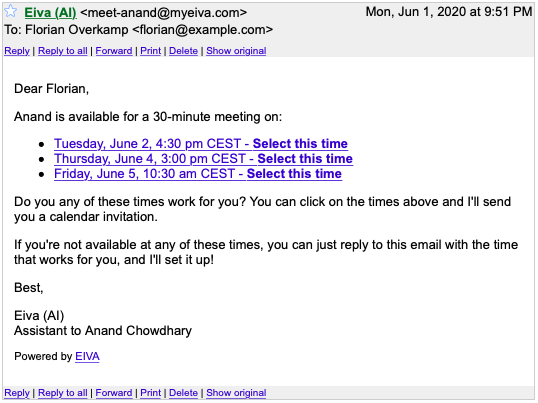
\includegraphics[width=10cm]{screenshot-dates.png}
	\caption{Screenshot of Time Recommendation Email}
\end{figure}

After receiving the list of time recommendations from the assistants, guests can click on their preferred option for confirmation (Section 6.2.4), and an email with a calendar invitation is sent to both the host and the guests.

\subsection{Frontend Web App}

The frontend web app is built with web development best practices, ease of use, and accessibility in mind.

For example, the EIVA homepage receives a 100\% score in the Accessibility audit part of Webkit Developer Tools. Using Lighthouse, an automated performance auditing tool, its score is 61/100 for performance, 93/100 for accessibility, 100/100 for best practices, and 92/100 for SEO. Oswald Labs' web accessibility plugin is also implemented on every page, which helps people with dyslexia read more easily, amongst other features \cite{gupta_improving_2019}.

\subsubsection{Vue.js and Nuxt.js}

As described in Section 2.2.2, Vue.js is the frontend development framework of choice for developing the EIVA web app. However, when building large-scale apps, setting up processes for routing, state management, and deploying can take up a lot of time. Therefore, Nuxt.js, an open source framework built on top of Vue.js is used which has these features built-in. For example, Nuxt.js can automatically generate routes based on file names, and also supports TypeScript; it ``provides a simple and intuitive developper experience to prototype blazing fast modern web application" \cite{alexchopin_announcing_nodate}.

Custom middleware and plugins were created and added to Nuxt.js for features like click tracking (Section 7.2.3), unauthenticated redirects, and persisted state (Section 6.2.3).

\paragraph{Fetch Requests}

The authentication process grants an access and a refresh token on successful login (Section 6.1.4), which is stored centrally in the web app. HTTP requests to the API have the \texttt{Authorization} header consisting of the access token when the user is logged in. Requests are sent using Axios, a Promise-based HTTP client built on top of  \texttt{XMLHTTPRequest}.

\paragraph{State Management}

A central store was used for authentication, consisting of both tokens and details about the logged in user, such as their memberships. \emph{Vuex}, Vue.js's state management pattern and library, is used with types and rulesets ensuring that the state can only be mutated in a predictable fashion. The store is also persisted locally in the browser's local storage as a JSON object, so that authentication details are not lost if the user closes and returns to the web app at a later time.

\subsubsection{User Interface}

The web app UI was wireframed, prototyped, and mocked up extensively before implementation (Section 4.3). It consists of simple branding and a color scheme focusing on desired actions. Figures 15 to 20 show the screenshots of important webpages.

\begin{figure}[h]
  \makebox[\textwidth]{%
    \begin{minipage}[t]{0.8\textwidth}
      \centering
      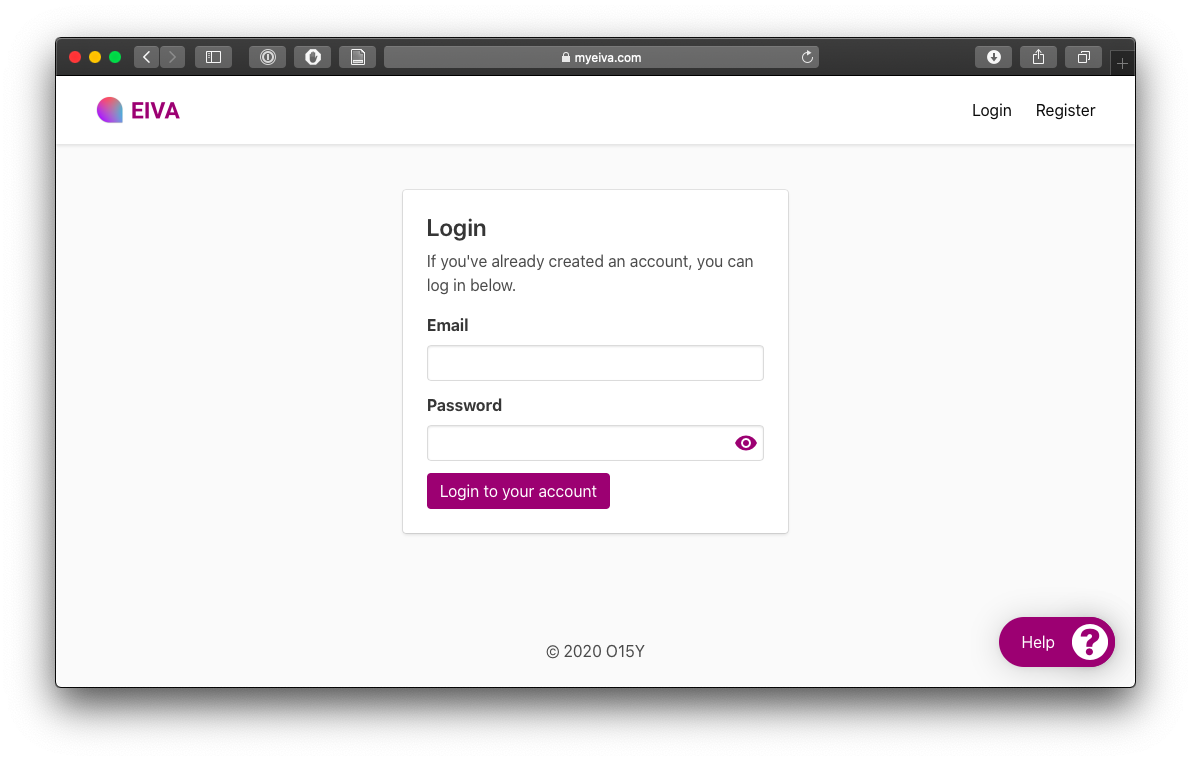
\includegraphics[width=\textwidth]{screenshot-login.png}
      \caption{Screenshot of Login Page}
    \end{minipage}%
    \hfill
    \begin{minipage}[t]{0.8\textwidth}
      \centering
      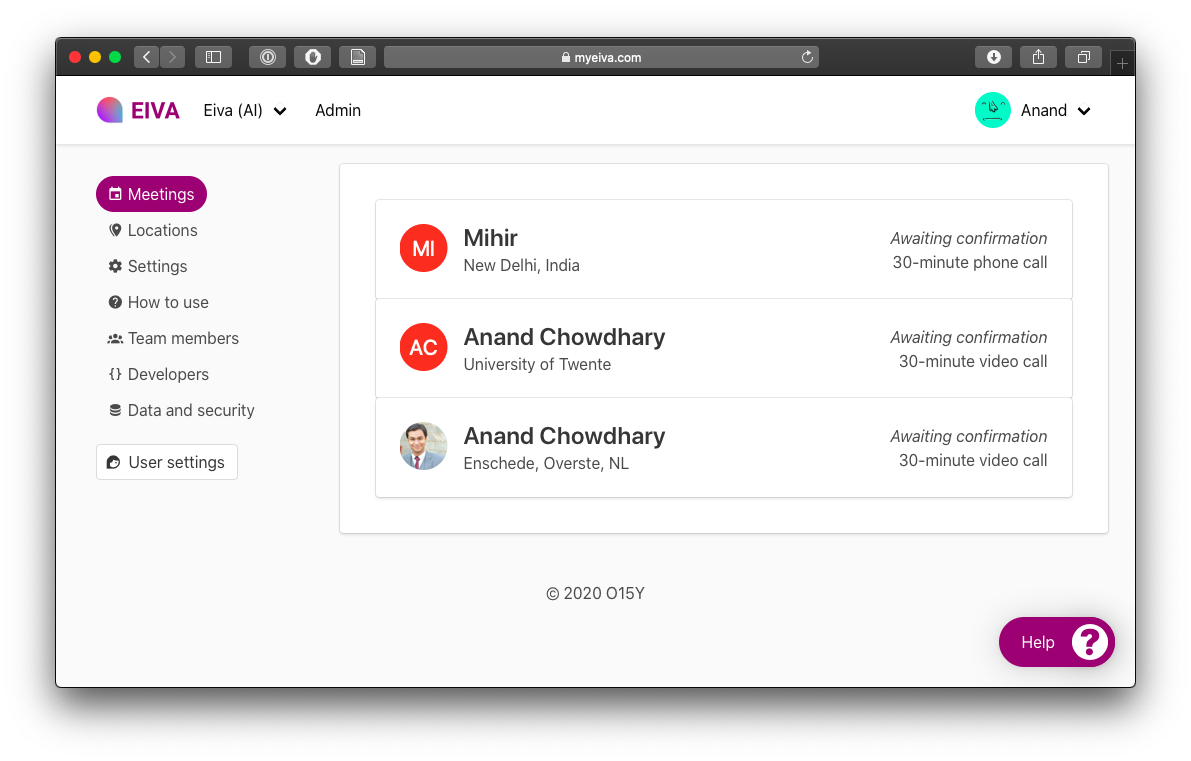
\includegraphics[width=\textwidth]{screenshot-meetings.png}
      \caption{Screenshot of Meetings Page}
    \end{minipage}%
  }%
\end{figure}
\begin{figure}[h!]
  \makebox[\textwidth]{%
    \begin{minipage}[t]{0.8\textwidth}
      \centering
      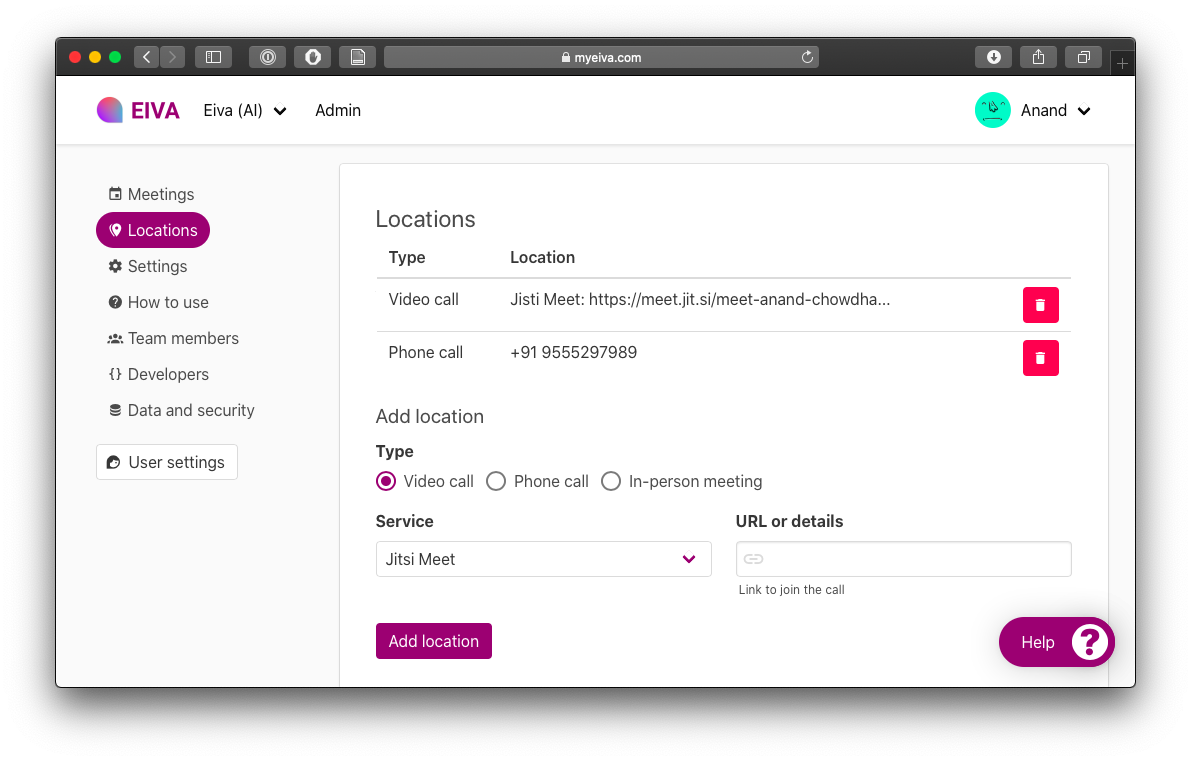
\includegraphics[width=\textwidth]{screenshot-locations.png}
      \caption{Screenshot of Locations Page}
    \end{minipage}%
    \hfill
    \begin{minipage}[t]{0.8\textwidth}
      \centering
      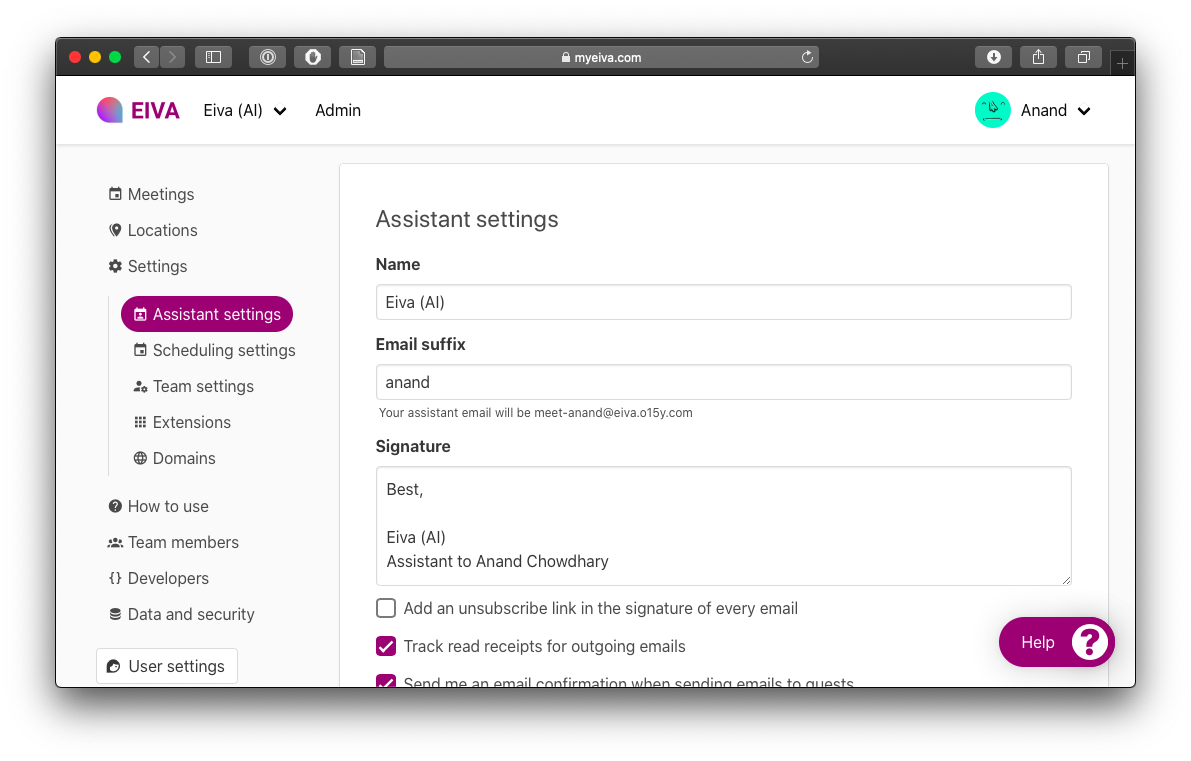
\includegraphics[width=\textwidth]{screenshot-assistant.png}
      \caption{Screenshot of Assistant Settings}
    \end{minipage}%
  }%
\end{figure}
\begin{figure}[h!]
  \makebox[\textwidth]{%
    \begin{minipage}[t]{0.8\textwidth}
      \centering
      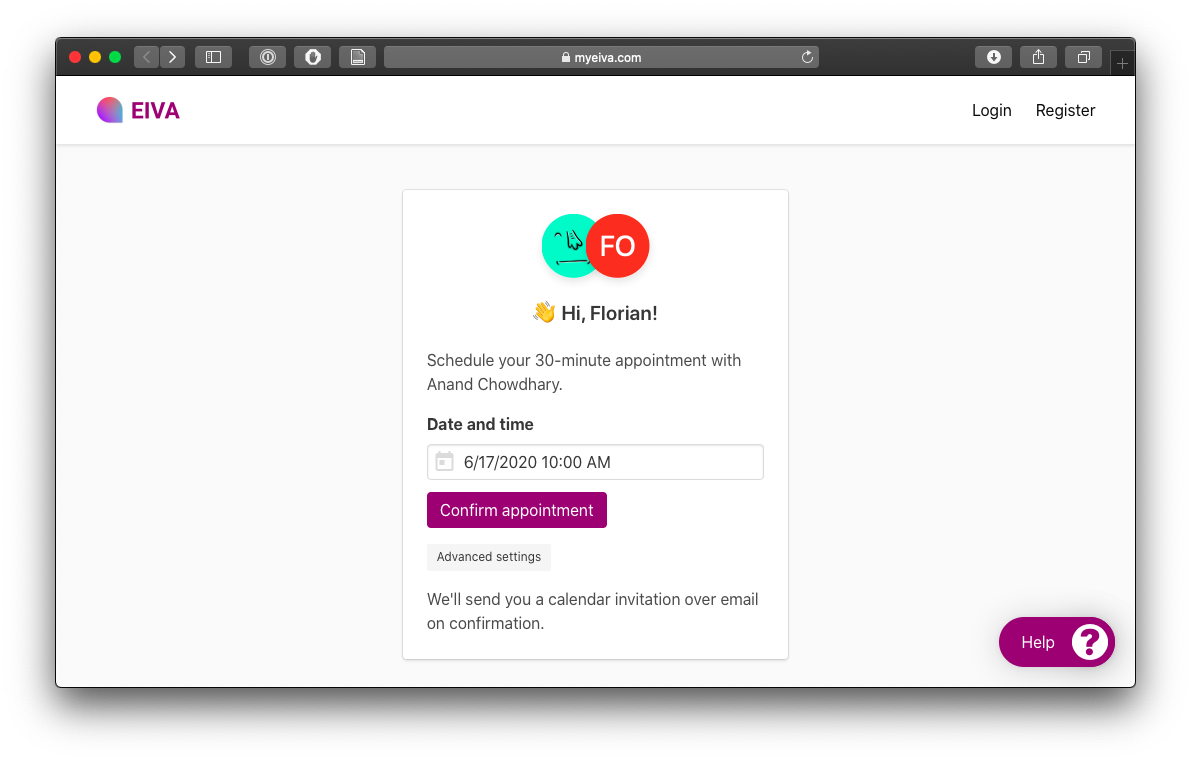
\includegraphics[width=\textwidth]{screenshot-confirm.png}
      \caption{Screenshot of Confirmation Page}
    \end{minipage}%
    \hfill
    \begin{minipage}[t]{0.8\textwidth}
      \centering
      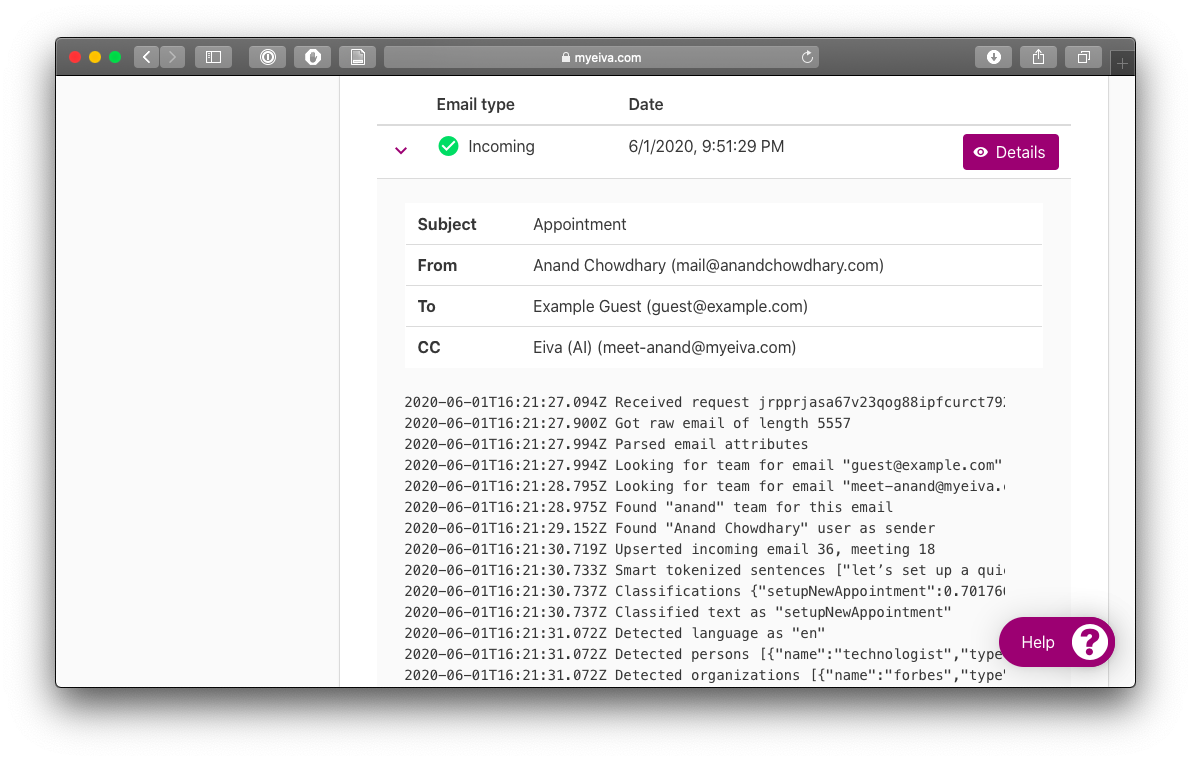
\includegraphics[width=\textwidth]{screenshot-logs.png}
      \caption{Screenshot of Incoming Email Logs Page}
    \end{minipage}%
  }%
\end{figure}
\begin{figure}[h!]
  \makebox[\textwidth]{%
    \begin{minipage}[t]{0.8\textwidth}
      \centering
      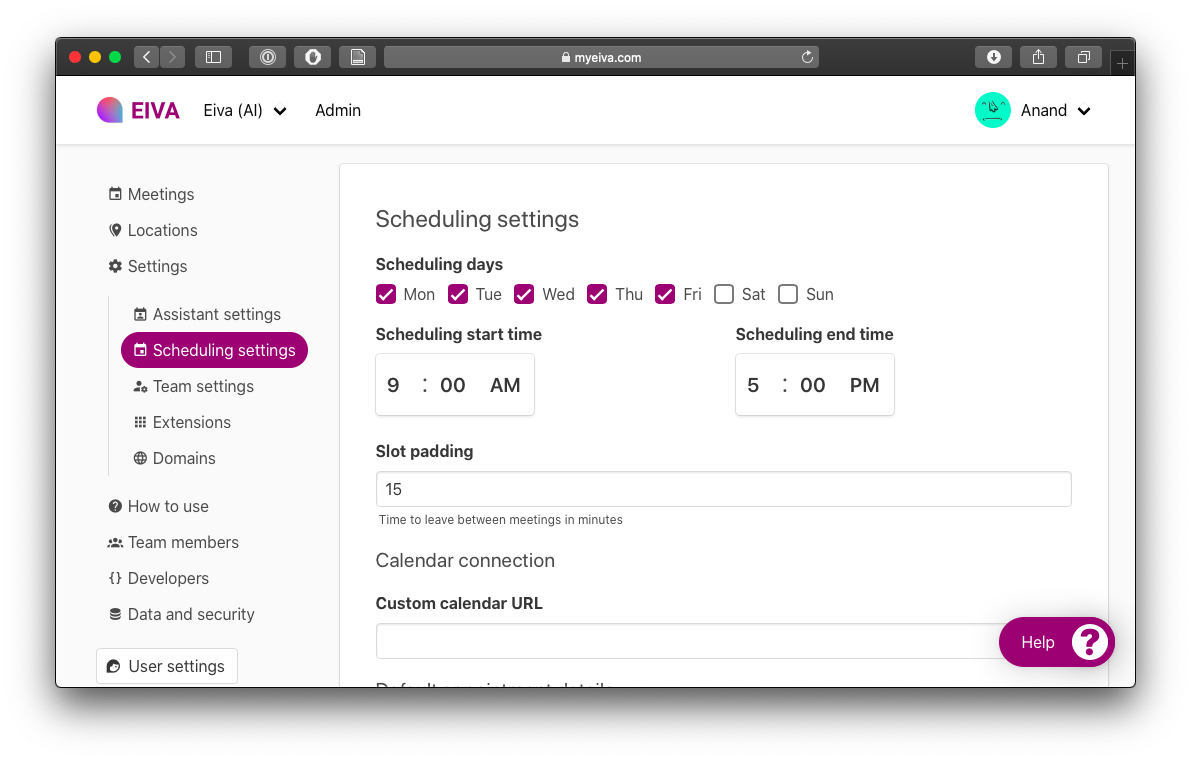
\includegraphics[width=\textwidth]{screenshot-scheduling.png}
      \caption{Screenshot of Scheduling Settings}
    \end{minipage}%
    \hfill
    \begin{minipage}[t]{0.8\textwidth}
      \centering
      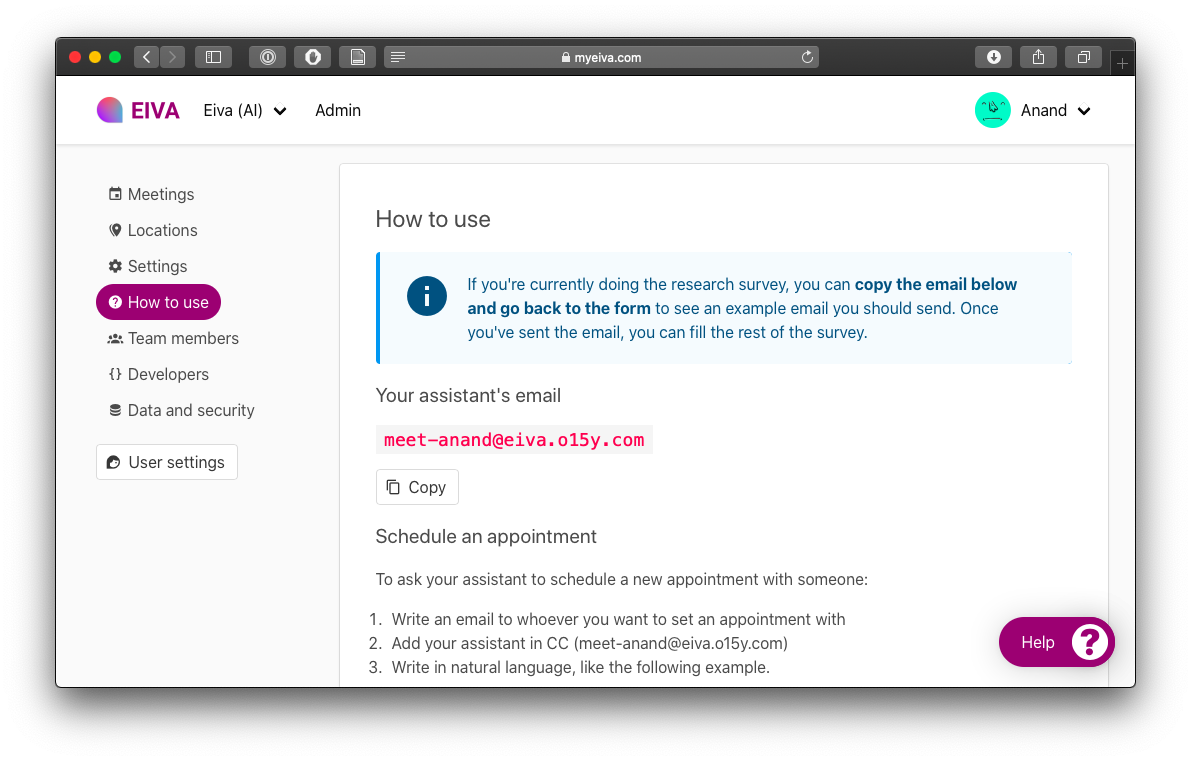
\includegraphics[width=\textwidth]{screenshot-how-to-use.png}
      \caption{Screenshot of How to Use Page}
    \end{minipage}%
  }%
\end{figure}

\subsection{Product Development Cycle}

During development, a simplified version of the Software Development Life Cycle and the New Product Development Process were adopted for this project, with the following steps:

\begin{enumerate}
	\item Idea
	\item Research
	\item Development
	\item External testing
	\item Analysis
\end{enumerate}

The first step builds on top of the ideation phase with methodological exploration of the idea and specifying the required feature as a module. In the second step, the technical literature research present in Section 2 is studied to architect the module's technology. In the third step, the idea is materialized by writing code and testing the module by writing unit tests and conducting end-to-end tests with the platform. In the fourth step, a test is conducted with the client or research participants. In the last step, the feedback from the test is evaluated for the next cycle.

\begin{figure}
	\centering
	\begin{minipage}{.4\textwidth}
		\centering
		
\includegraphics[height=.75\linewidth]{software-cycle.png}
		\captionof{figure}{The Software Development Cycle \cite{vlasova_7_nodate}}
		\label{fig:test1}
	\end{minipage}%
	\hspace{.5cm}
	\begin{minipage}{.4\textwidth}
		\centering
		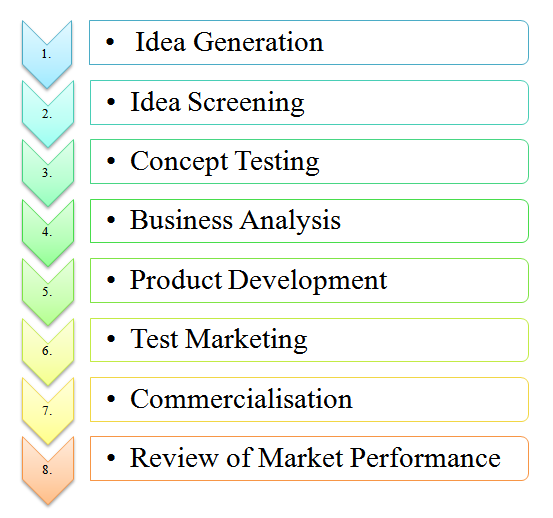
\includegraphics[height=.75\linewidth]{product-cycle.png}
		\captionof{figure}{The New Product Development Process \cite{akrani_stages_nodate}}
		\label{fig:test2}
	\end{minipage}
\end{figure}

\subsubsection{Cycle 1: Assistant Email Address}

The first cycle was internal with both the initial development and several refactors. One of the specified conditions in Section 3 was to ensure unique email addresses for each organization using the assistant service, because teams may have similar names of assistants. For example, the default name of the assistant, \emph{Ara Isaacson (AI)}, may generate the email address \texttt{ara@example.com}, which does not share any information about who the assistant works for. Since unique email addresses for each team is mandatory, the team's slug was incorporated in the address, i.e., \texttt{username@example.com}, for example \texttt{florian@example.com}. 

This has two advantages: firstly, it tells the guests receiving emails from the assistant who the true host is; and secondly, the email receiving architecture can relate the unique email address to the owner's details. However, this might be mistaken as the email address of the user themselves (for example, Florian) rather than their assistant. Therefore, the last change was to add the suffix, \texttt{meet-} to each email, e.g., \texttt{meet-florian@example.com}.

\subsubsection{Cycle 2: Onboarding Interface}

In the second cycle, the client's feedback was that users should have a simpler experience when signing up for the EIVA service. Although sensible defaults have been implemented, users may get overwhelmed with several privacy settings, so this should be simplified in an onboarding experience.

Therefore, an onboarding experience was designed where users could easily set their basic information, and select one of three privacy options. Figure 23 and 24 show the updated onboarding interface for user and privacy settings respectively.

\begin{figure}[h]
  \makebox[\textwidth]{%
    \begin{minipage}[t]{0.8\textwidth}
      \centering
      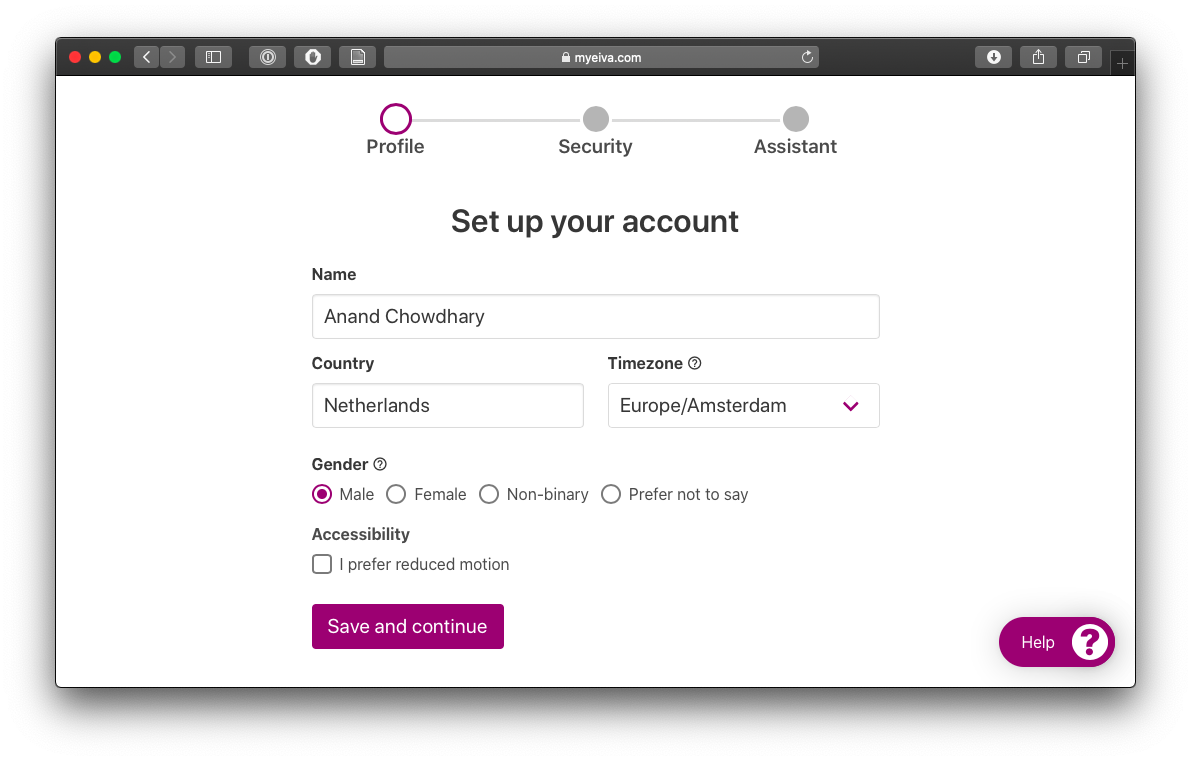
\includegraphics[width=\textwidth]{screenshot-onboarding-1.png}
      \caption{Screenshot of Scheduling Settings}
    \end{minipage}%
    \hfill
    \begin{minipage}[t]{0.8\textwidth}
      \centering
      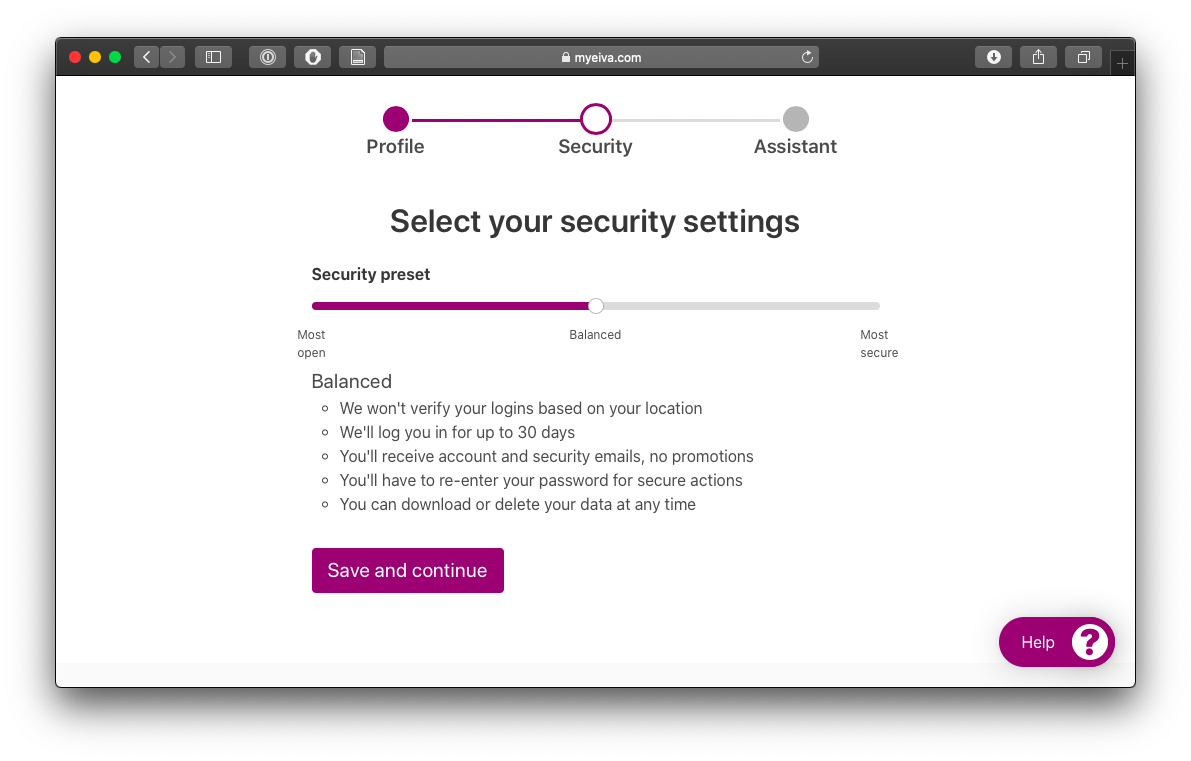
\includegraphics[width=\textwidth]{screenshot-onboarding-2.png}
      \caption{Screenshot of How to Use Page}
    \end{minipage}%
  }%
\end{figure}

A slider interface was implemented for privacy settings, with `Most open', `Balanced', and `Most secure' options. Selecting one of these three options would configure several settings, such as whether to verify logins based on location, whether to receive promotional emails, etc.

\subsubsection{Cycle 3: iCalendar Support}

The assumption that most users would use Google Calendar ensured that development time was spent on easy connectivity with Google accounts. The official Google Calendar API was used to fetch events when recommending time slots using the open source package \texttt{calendar-slots} (Section 6.4). However, this meant that non-Google users could not connect their calendars, and the client themselves uses a self-hosted calendar system. It was therefore recommended to support other calendars that support the iCalendar specification.

Most calendar services are compliant with iCalendar, therefore adding first-class support for iCalendar URLs meant that users using almost any digital calendar could have event conflict resolution features. ICS support was implemented and Google's API was also replaced with the new system. In Figure 19, users are asked to enter an iCalendar URL rather than connecting their Google accounts.

\subsubsection{Cycle 4: Dutch Training Data}

EIVA only worked in English until Cycle 4, and it was recommended by the client to add natural-language capabilities in multiple languages, especially Dutch. The initial idea was to use a translation API such as Google Translate to first translate incoming emails to English, and then continue processing the email. However, this was troublesome, because imperfect translations did not receive high classification scores in the NLP engine trained with English data.

It was decided to have first-class support for both English and Dutch, and therefore a new Dutch training dataset was added. The process also added a language detection step, so incoming emails in English or Dutch would use their own respective NLP classifiers before continuing with the scheduling process. This ensures equally high accuracy in both languages.

\subsubsection{Cycle 5: Bugs and New Domain}

In Cycle 5, the client was able to extensively use EIVA and found several bugs and enhancement recommendation. First, an error was found where deleting the default location (an auto-generated Jitsi Meet link) would throw an error. This was fixed by adding support for custom default meeting locations and automatically changing the default location in case the current default is deleted by the user. Secondly, the client recommended removing HTTP access and redirecting all requests to the secure HTTPS protocol, which was implemented. Several other bugs were also fixed during this feedback cycle.

Also, the website was migrated to the new domain \texttt{myeiva.com} (a different domain was used during development), but this had an email deliverability error. Since the domain was purchased on June 1, 2020, email clients were marking emails from EIVA under `Spam' because the domain was too new. Therefore, the website remained hosted on the new domain, but the assistant emails were moved for the testing period from \texttt{@myeiva.com} to \texttt{@eiva.o15y.com}. \texttt{o15y.com} was purchased over two years ago and therefore had more credibility.

\subsubsection{Cycle 6}

In the final feedback stage, three experienced web developers --- Alex Imbrea, Maurits van der Vijgh , Rohit Bhatia --- were asked to use the EIVA webapp and assistant and provide additional feedback. Their suggestions included adding input validation on the client side for the minimum password length of 6 characters, which was only imposed on the server side. They also thought that the intro tour was too long, described as ``hand holding", though they agreed that it was necessary for users without a technical background.

A grammatical error was also found in the outbound email sent by the assistant, and another error that prevented cache invalidation. They were both fixed and deployed before testing with users (Section 7).

\subsection{Open Source Development}

Although the preceding project Ara was licensed under the permissive MIT license, EIVA's source code is made available under the Server Side Public License (SSPL). SSPL makes sure that any further implementations or paid services built around EIVA also have their source code made public, meaning that companies will not be able to sell competing services using EIVA's publicly-available source code. This was selected to help the future business case.

Nevertheless, several open source projects were built in order to support key EIVA features, and were all licensed under the MIT license. This encourages wide community adoption and contributes back to the open source ecosystem. MIT is the most popular open source license and it allows commercial usage of all code, so competing services are also free to use this package in the future.

\paragraph{Calendar Link}

For example, the open source project \texttt{calendar-link} was built in order to generate event links to popular calendar services like Google Calendar, Microsoft Outlook, and Yahoo! Calendar. This project is now used by many others, receiving over 1,000 downloads every week and contributed to by 5 additional developers. Developers can use the package to programmatically generate that users can click on to add a specific event to their calendar, with an easy-to-use API.

\begin{alltt}
\textcolor{keyword}{import} \{ google, outlook, ics \} \textcolor{keyword}{from} \textcolor{string}{"calendar-link"};
\textcolor{keyword}{const} event = \{
  \textcolor{symbol}{title}: \textcolor{string}{"My birthday party"},
  \textcolor{symbol}{start}: \textcolor{string}{"2020-12-29 18:00:00 +0100"},
  \textcolor{symbol}{duration}: [\textcolor{literal}{3}, \textcolor{string}{"hour"}]
\};
\textcolor{variable}{google}(event); \textcolor{comment}{// https://calendar.google.com/calendar/...}
\textcolor{variable}{outlook}(event); \textcolor{comment}{// https://outlook.live.com/owa/...}
\textcolor{variable}{ics}(event); \textcolor{comment}{// BEGIN:VCALENDAR VERSION:2.0...}
\end{alltt}

\paragraph{Calendar Slots}

Similarly, another project \texttt{calendar-slots} was released to help find available slots in a user's calendar. This package can save development times when recommending appointment slots by listing a user's calendars, fetching all events in a given timeframe, removing slots with conflicts with scheduled events, and recommending a fixed number of slots to the end user:

\begin{alltt}
\textcolor{keyword}{import} \{ findSlots \} \textcolor{keyword}{from} \textcolor{string}{"calendar-slots"};
\textcolor{keyword}{const} tomorrow = \textcolor{keyword}{new} Date();
\textcolor{keyword}{const} slots = \textcolor{keyword}{await} \textcolor{variable}{findSlots}(\{
  \textcolor{symbol}{slotDuration}: \textcolor{literal}{30}, \textcolor{comment}{// Find 30 minute slots}
  \textcolor{symbol}{slots}: \textcolor{literal}{3}, \textcolor{comment}{// Recommend 3 slots}
  \textcolor{symbol}{from}: \textcolor{keyword}{new} Date(), \textcolor{comment}{// Starting now}
  \textcolor{symbol}{to}: tomorrow.\textcolor{variable}{setDate}(today.\textcolor{variable}{getDate}() + \textcolor{literal}{1}), \textcolor{comment}{// Until tomorrow}
\});
\end{alltt}

EIVA uses this package under the hood to recommend time slots for appointments. It is also highly configurable, with support for settings such as timezone preference, daily scheduling hours, and custom filter options:

\begin{alltt}
\textcolor{keyword}{import} moment from \textcolor{string}{"moment"};
\textcolor{keyword}{const} slots = \textcolor{keyword}{await} \textcolor{variable}{findSlots}(\{
  \textcolor{symbol}{slotDuration}: \textcolor{literal}{30}, \textcolor{comment}{// Find 30 minute slots}
  \textcolor{symbol}{slots}: \textcolor{literal}{3}, \textcolor{comment}{// Recommend 3 slots}
  \textcolor{symbol}{from}: moment(), \textcolor{comment}{// Starting now}
  \textcolor{symbol}{to}: moment().\textcolor{variable}{add}(\textcolor{literal}{1}, \textcolor{string}{"week"}), \textcolor{comment}{// Until next week}
  \textcolor{symbol}{days}: [\textcolor{literal}{1}, \textcolor{literal}{2}, \textcolor{literal}{3}, \textcolor{literal}{4}, \textcolor{literal}{5}], \textcolor{comment}{// Only on week days}
  \textcolor{symbol}{daily}: \{ \textcolor{comment}{// Make sure all these conditions are met}
    \textcolor{symbol}{timezone}: \textcolor{string}{"Europe/Amsterdam"}, \textcolor{comment}{// Set CET timezone}
    \textcolor{symbol}{from}: [\textcolor{literal}{9}], \textcolor{comment}{// Start at 09:00 in the morning}
    \textcolor{symbol}{to}: [\textcolor{literal}{17}, \textcolor{literal}{30}], \textcolor{comment}{// End at 17:30 in the evening}
  \}
\});
\end{alltt}

Both projects are written in TypeScript and available on the Git hosting service GitHub and JavaScript package registry npm.

\subsection{Software Tests}

\subsubsection{Unit Tests}

Unit tests, a method to test individual units of code, are used to ensure all components are behaving as intended \cite{tosun_effectiveness_2018}. The goal of unit testing is to isolate each part of the code and ensure that individual parts are correct, before writing comprehensive tests for an entire module.

For example, the \texttt{dates.spec.ts} file consists of 5 tests for the date parser. Each test provides a strict, written contract that the \texttt{findStartEndTime} function must satisfy. This function takes a string of text and returns the start and end time for scheduling. For example, the input ``set up an appointment for next week" will return the start time of the following Monday 00:00 and end time of Sunday 23:59, whereas the input of ``set up an appointment for tomorrow" will return the start and end time for the following day.

During development, such methods are used extensively to test the natural language processing by supplying many different strings and programmatically testing their outputs. The testing framework \emph{Jest} is used with an npm script for automated testing.

\subsubsection{Continuous Integration}

A Continuous Integration (CI) process consisting of unit tests and a build test has been set up to ensure that no bad code gets deployed to users \cite{li_extensive_2020}. Whenever a new commit is pushed to the central repository on GitHub, the code is only deployed to the production app when there is a successful build \cite{noauthor_what_2019}.

GitHub Actions is used as the API for CI, and is free for public repositories. A workflow consisting of 5 steps is triggered on every push, using Ubuntu  18.04 LTS, a popular Linux distribution:

\begin{enumerate}
	\item Checkout the repository (using \texttt{actions/checkout@v2})
	\item Setup Node.js v14.3 (using \texttt{actions/setup-node@v1})
	\item Install dependencies (\texttt{npm ci})
	\item Run all unit tests (\texttt{npm run test})
	\item Compile the TypeScript project (\texttt{npm run build})
\end{enumerate}

When there is an error in the build such as if a unit test fails or there is a TypeScript compilation error, the pipeline fails and developers get a notification for error mitigation. On average this CI process takes 2 minutes to complete, and Figure 11 shows the duration of each workflow run.

\begin{figure}[h]
	\centering
	\begin{minipage}{.47\textwidth}
		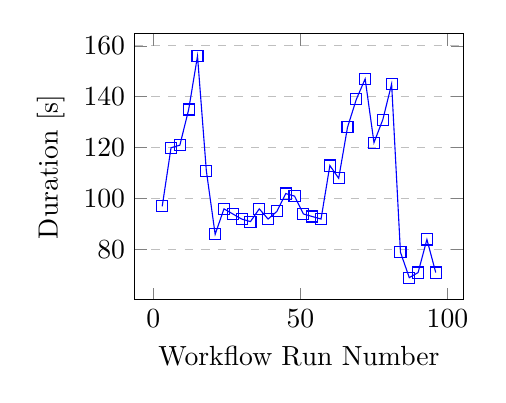
\begin{tikzpicture}
			\begin{axis}[
					width=5.75cm,
					xlabel={Workflow Run Number},
					ylabel={Duration [s]},
					legend pos=north west,
					ymajorgrids=true,
					grid style=dashed,
				]
				\addplot[
					color=blue,
					mark=square,
				]
				coordinates {
					(3, 97)(6, 120)(9, 121)(12, 135)(15, 156)(18, 111)(21, 86)(24, 96)(27, 94)(30, 92)(33, 91)(36, 96)(39, 92)(42, 95)(45, 102)(48, 101)(51, 94)(54, 93)(57, 92)(60, 113)(63, 108)(66, 128)(69, 139)(72, 147)(75, 122)(78, 131)(81, 145)(84, 79)(87, 69)(90, 71)(93, 84)(96, 71)
				};
				
			\end{axis}
		\end{tikzpicture}
		\caption{Running Time of Continuous Integration Workflows}
	\end{minipage}
	\hspace{.5cm}
	\begin{minipage}{.47\textwidth}
		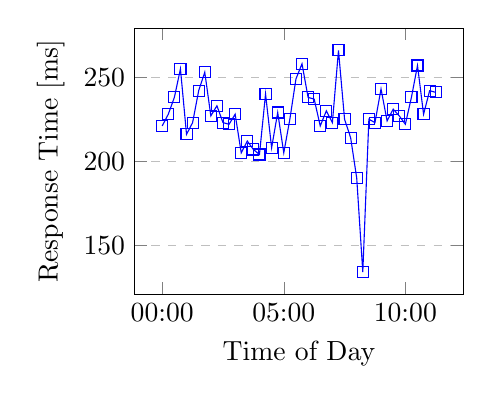
\begin{tikzpicture}
			\begin{axis}[
					width=5.75cm,
					xlabel={Time of Day},
					ylabel={Response Time [ms]},
					legend pos=north west,
					ymajorgrids=true,
					grid style=dashed,
					xticklabels={0,00:00,05:00,10:00,15:00,20:00}
				]
				\addplot[
					color=blue,
					mark=square,
				]
				coordinates {
					(0, 221)(1, 228)(2, 238)(3, 255)(4, 216)(5, 223)(6, 242)(7, 253)(8, 227)(9, 233)(10, 223)(11, 222)(12, 228)(13, 205)(14, 212)(15, 207)(16, 204)(17, 240)(18, 208)(19, 229)(20, 205)(21, 225)(22, 249)(23, 258)(24, 238)(25, 237)(26, 221)(27, 230)(28, 223)(29, 266)(30, 225)(31, 214)(32, 190)(33, 134)(34, 225)(35, 223)(36, 243)(37, 224)(38, 231)(39, 227)(40, 222)(41, 238)(42, 257)(43, 228)(44, 242)(45, 241)
				};
			\end{axis}
		\end{tikzpicture}
		\caption{24-Hour Response Time of the EIVA website}
	\end{minipage}%
\end{figure}

\subsubsection{Initialization Tests}

Lastly, initialization tests are used after deploying the app to ensure that all services are functioning. The \texttt{init-test.ts} file has 6 tests that run as soon as the app is launched. If there is an error with any of these services, it is immediately logged in the console. The output of a successful initialization is shown in Figure 16. After the server is ready, the connection to self-hosted services like Redis and MariaDB are tested; then, a test email is sent to ensure outbound emails are delivered; finally, the connection to third-party services like Stripe and ElasticSearch is tested.

\begin{figure}[h]
	\center
	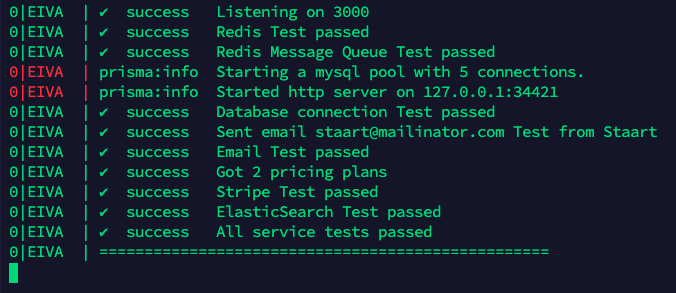
\includegraphics[width=10cm]{init-tests.png}
	\caption{Successful Initialization Tests}
\end{figure}

\subsection{Deployment}

Amazon Web Services (AWS) resources are used for deploying the backend project. AWS is highly scalable and has an easy-to-use admin portal to manage resources and billing \cite{shokeen_deploying_2019}. AWS is also one of the most secure cloud computing platforms \cite{narula_cloud_2015}. For minimal latency and data storage compliance, the Frankfurt AWS Infrastructure Region was selected. Therefore, no data ever leaves the European Union.

\subsubsection{Infrastructure Cost}

The total infrastructure cost between May and July 2020 was approximately US\$300. However, the entire cost was subsidized in the form of AWS credits, generously provided by Oswald Labs, the researcher's company, with the exception of the domain name \cite{noauthor_oswald_nodate}. The \texttt{myeiva.com} domain was purchased through Hover and costed US\$12.99. All AWS services were billed from May 21, 2020 to July 21, 2020.

\paragraph{Server}

A dedicated server is used for deploying the EIVA backend. This uses AWS Lightsail which provides an easy-to-use interface for AWS EC2, with the following instance details. The cost of this server was US\$20 per month:

\begin{itemize}
	\item RAM: 4 GB
	\item Processor: 2 vCPUs
	\item Storage: 80 GB SSD
\end{itemize}

\paragraph{ElasticSearch}

A dedicated ElasticSearch instance is used to store server logs and track usage events, with the following instance details. The total cost of this instance was US\$272, billed as US\$0.186 per hour:

\begin{itemize}
	\item Elasticsearch version: 7.4
	\item Instance type: r5.large.elasticsearch
	\item EBS volume size: 10 GiB
\end{itemize}

\subsubsection{Backend APIs}

To deploy the backend APIs, a custom shell script was written that fetches code from the git repository, installs dependencies, and runs the project. The \texttt{update.sh} file consists of the following lines:

\begin{alltt}
git pull --force \textcolor{comment}{# Pull code from GitHub}
npm install \textcolor{comment}{# Install npm dependencies}
npx prisma generate \textcolor{comment}{# Generate database schema}
npm run build \textcolor{comment}{# Compile TypeScript project}
pm2 flush \textcolor{comment}{# Clear current deployment's logs}
pm2 restart all \textcolor{comment}{# Restart all services}
pm2 logs \textcolor{comment}{# Show the logs of this deployment}
\end{alltt}

\subsubsection{Frontend Web App}

Deploying the frontend web app is much easier because of the CI process. The frontend is hosted on the static site hosting platform \emph{Netlify}, which automatically build and deploys the app on push. This service is also free.

\subsubsection{Server Monitoring}

\paragraph{Uptime Monitoring}

Although measures have been taken to make sure EIVA services don't go down, such as installing Cloudflare' Always Online which serves a static version of a webpage if it is not available from the origin server \cite{noauthor_keep_nodate}, there is sometimes nothing one can do to prevent a website from going down. ``Traffic spikes, malware attacks, data center problems, etc." can cause server downtime \cite{noauthor_what_2018}.

To monitor the uptime of the services and get real-time notifications in case of downtime, \emph{Uptime Robot} is installed \cite{noauthor_about_nodate}. In intervals of 5 minutes, Uptime Robot makes network requests to the frontend and backend URLs, logs the response time (Figure), and sends an email and Slack notification in case any URL is unavailable.

Over the course of testing weeks, no downtime was recorded for the backend, but the frontend was unavailable twice for a period of 2 minutes and 57 seconds and 2 minutes and 44 seconds on June 7 and June 9 2020 respectively. This was due of a Netlify deploying error because of renamed repositories. Both times, this error was immediately fixed because of the real-time notifications feature, and resulted in a $>$ 99.98\% overall uptime.

\paragraph{Resource Monitoring}

To make sure the service is not over used and to prevent crashes, \emph{Netdata} is used to monitor all aspects of the server. Netdata can visualize and monitor real-time metrics, optimized to accumulate all types of data, such as CPU usage, RAM usage, and disk activity \cite{noauthor_netdata_nodate}. NetData is also open source and consists of a daemon that collects collecting and an interface to visualize that data \cite{noauthor_netdata/netdata_2020}.

\paragraph{Error Tracking}

To catch errors in production, \emph{Sentry} is deployed in both the frontend and backend applications. Sentry is an open source error tracking system \cite{noauthor_sentry_nodate} that automatically reports errors as soon as they occur. ``In addition to sending developers alerts, Sentry also gives them context for potential root cause analysis to help them identify the source of the error" \cite{noauthor_sentry_nodate-1}.

Although the backend project collects server logs, they are frequently intentional debugging information. Logging provides a trail of events, but Sentry only focuses on exceptions, i.e., catching application crashes or HTTP request errors. Furthermore, Sentry helps list a trail of usage events like mouse clicks and network requests to discover the context of an error \cite{noauthor_sentry_nodate-2}.

Licensed under Apache 2, Sentry is open source but offers a hosted service with a generous free plan, which is used for this project. The @sentry/browser package is used to track errors originating in client-side web applications running in browsers, and @sentry/node is used for the Node.js package.

Over the course of testing weeks, 3 errors were tracked for the frontend project, but no errors were found in the backend project.

\newpage

\section{Evaluation}

The goal of this user experience evaluation was to allow 30 users to create their own assistants using the EIVA service and use the companion app before hearing their feedback. The form opened on June 1, 2020, and was closed on June 24, 2020, when 30 responses had been recorded.

\subsection{Introductory Survey}

A diverse group of users participated in the survey, both working professionals and students. 18 out of 30 respondents were professionals employed full-time by a company or organization, another 9 were students, and 3 out of 30 were freelancers or self-employed individuals (Table 1).

\begin{table}[!htb]
	\begin{minipage}{.5\linewidth}
		\caption{Professions of Participants}
		\centering
		\begin{tabular}{lr}
			\hline
			\textbf{Profession} & \textbf{Count} \\
			\hline
			Employed            & 18             \\
			Student             & 9              \\
			Self-employed       & 3              \\
			\hline
		\end{tabular}
	\end{minipage}%
	\hspace{.1cm}
	\begin{minipage}{.5\linewidth}
		\centering
		\caption{Preferred Modes of Scheduling}
		\begin{tabular}{lr}
			\hline
			\textbf{Mode}        & \textbf{Count} \\
			\hline
			Send an email        & 24             \\
			Work chat message    & 12             \\
			Go to office or desk & 12             \\
			Phone call           & 9              \\
			Consumer chat        & 8              \\
			\hline
		\end{tabular}
	\end{minipage}
\end{table}

User were also asked their preferred modes of scheduling. In Table 2, `Work chat' refers to instant messaging services like Slack and Microsoft Teams whereas `Consumer chat' refers to services like WhatsApp and Facebook Messenger, and participants could choose multiple options. The results show a preference for emails, as noted in Section 2. Apart from email, work chat services or physically reaching out are popular too, whereas phone calls and consumer chat services are used least frequently.

\subsubsection{Email and Calendar Usage}

To ensure that email is the ideal use case for scheduling, participants were asked about their frequency of sending emails (Table 3) and checking their email (Table 4). More than half of all participants send multiple emails per day, whereas almost one third send an email once every few days. Only 3 and 2 respondents send an email once every few weeks or per month respectively. Almost two thirds of all participants check their email multiple times per day, and 7 out of 30 said that they check it at least once per day. 4 and 1 participant(s) check their email at least weekly and monthly respectively. Therefore, large a majority of all participants both frequently send and check for emails.

\begin{table}[!htb]
	\begin{minipage}{.5\linewidth}
		\caption{Frequency of Emails Sent}
		\centering
		\begin{tabular}{lr}
			\hline
			\textbf{Number of Emails} & \textbf{Count} \\
			\hline
			One or more per day       & 16             \\
			One every few days        & 9              \\
			One every few weeks       & 3              \\
			One every month           & 2              \\
			\hline
		\end{tabular}
	\end{minipage}%
	\hspace{.1cm}
	\begin{minipage}{.5\linewidth}
		\centering
		\caption{Frequency of Checking Email}
		\begin{tabular}{lr}
			\hline
			\textbf{Number of Times} & \textbf{Count} \\
			\hline
			Multiple times per day   & 18             \\
			At least once per day    & 7              \\
			At least once per week   & 4              \\
			At least once per month  & 1              \\
			\hline
		\end{tabular}
	\end{minipage} 
\end{table}

Since EIVA supports both English and Dutch, participants were asked their preferred languages for email communication. All 30 participants selected English, 9 participants also chose Dutch, and 1 participant also selected German and Polish each.

For better integration with large email providers, participants were also asked about their primary email service provider. Over half of all participants use Google's Gmail or G Suite (17), 8 in 30 use a Microsoft service (like Hotmail or Live), 2 use each of custom hosted SMTP or others, and 1 respondent uses Yahoo!.

Furthermore, they were asked whether they have email notifications enabled on their smartphones, to which all but three participants responded in the affirmative. This shows that an overwhelming majority of users check their email frequently and receive email notifications.

\begin{table}[!htb]
	\begin{minipage}{.5\linewidth}
		\caption{Email Languages}
		\centering
		\begin{tabular}{lr}
			\hline
			\textbf{Language} & \textbf{Count} \\
			\hline
			English           & 30             \\
			Dutch             & 9              \\
			German            & 1              \\
			Polish            & 1              \\
			\hline
		\end{tabular}
	\end{minipage}%
	\hspace{.1cm}
	\begin{minipage}{.5\linewidth}
		\centering
		\caption{Email Service Providers}
		\begin{tabular}{lr}
			\hline
			\textbf{Service} & \textbf{Count} \\
			\hline
			Google           & 17             \\
			Microsoft        & 8              \\
			SMTP             & 2              \\
			Other            & 2              \\
			Yahoo!           & 1              \\
			\hline
		\end{tabular}
	\end{minipage} 
\end{table}

Apart from scheduling, there are also several other reasons to use email. Participants were asked \emph{What do you use email for?}, and 29 out of 30 participants selected work-related communication. 16 participants also chose scheduling appointments, while 5 in 30 use email to connect with friends and family. 3 out of 30 participants use email for outbound marketing, whereas 1 also uses it for customer support.

\begin{table}[!htb]
	\begin{minipage}{1\linewidth}
		\caption{Reasons for Sending Emails}
		\centering
		\begin{tabular}{lr}
			\hline
			\textbf{Reason}                         & \textbf{Count} \\
			\hline
			Other work-related communication        & 29             \\
			Scheduling appointments                 & 16             \\
			Connecting with friends and family      & 5              \\
			Sending marketing emails or newsletters & 3              \\
			Contacting customer support             & 1              \\
			\hline
		\end{tabular}
	\end{minipage}%
\end{table}

Although EIVA connects with any calendar application that follows the iCalendar standard, which all major services do, it also directly integrates with Google Calendar using the official API (iCalendar support was added in Cycle 3, Section 6.3.3). This was chosen with the hypothesis that it's the most popular calendar service, which was proved to be true based on the participants' responses. Almost two-thirds of all participants (19) selected Google Calendar as their primary calendar service, 9 out of 30 participants use Microsoft Outlook, and another 8 use Apple Calendar. 3 participants used other calendar services. Lastly, 1 respondent each uses a self-hosted calendar or no calendar.

\begin{table}[!htb]
	\begin{minipage}{1\linewidth}
		\caption{Primary Calendar Services}
		\centering
		\begin{tabular}{lr}
			\hline
			\textbf{Calendar Service}         & \textbf{Count} \\
			\hline
			Google Calendar                   & 19             \\
			Microsoft Outlook                 & 9              \\
			Apple Calendar                    & 8              \\
			Other calendar app                & 3              \\
			Self-hosted calendar              & 1              \\
			\emph{I don't use a calendar app} & 1              \\
			\hline
		\end{tabular}
	\end{minipage}%
\end{table}

\subsubsection{Personal Assistant for Scheduling}

In the second part of the Introductory Survey, participants were asked hypotheticals about using an assistant for scheduling meetings. The results of the six polar questions (yes/no) are tabulated in Table 9.

\begin{table}[!htb]
	\begin{minipage}{1\linewidth}
		\caption{Responses to Polar Question}
		\centering
		\begin{tabular}{p{9cm}p{0.75cm}p{0.75cm}}
			\hline
			\textbf{Question}                                                                               & \textbf{Yes} & \textbf{No} \\
			\hline
			If you had a personal assistant, would you ask them to schedule your appointments for you?      & 27           & 3           \\
			Would you use the EIVA service?                                                                 & 24           & 6           \\
			Should EIVA inform recipients that it is not human?                                             & 23           & 7           \\
			Should recipients be able to unsubscribe from EIVA emails?                                      & 19           & 11          \\
			Would you like to know whether someone has seen an email sent by EIVA?                          & 22           & 8           \\
			If you have enabled email tracking, should recipients know that a read receipt has been shared? & 21           & 9           \\
			\hline
		\end{tabular}
	\end{minipage}%
\end{table}

Currently, EIVA only sets appointments but the big picture goal of EIVA is to automate several other workflows, like automatically responding to emails or sending outbound marketing emails. Participants were also asked what other features they would like to see.

Table 10 summarizes the most-requested additional features that participants want EIVA to have. 22 out of 30 respondents requested reminders, 17 out of 10 selected email follow-ups to team members, 15 out 30 selected automatic frequent email responses, 6 participants requested sending marketing emails. Two participants also added custom requests ``Send me my schedule at the start of my day" and ``Sort relevant emails, make summaries of long emails, and create a quick overview to-do list".

\begin{table}[!htb]
	\begin{minipage}{1\linewidth}
		\caption{Most Requested Additional Features}
		\centering
		\begin{tabular}{lr}
			\hline
			\textbf{Feature}                & \textbf{Count} \\
			\hline
			Reminders                       & 23             \\
			Send email follow-ups           & 17             \\
			Auto-respond to frequent emails & 15             \\
			Send marketing emails           & 6              \\
			\hline
		\end{tabular}
	\end{minipage}%
\end{table}

\subsection{Product Usage}

Data stored in ElasticSearch between June 1 and June 24 is analyzed, in which 30 participants used the product and responded to the questionnaire. In this period, a total of 2,244 pageviews and 19,177 API logs were collected.

\subsubsection{Web App Traffic Analysis}

As described in Section 6.5.3, a JavaScript snippet was used to send information about each pageview to the ElasticSearch engine via the API, and most data was computed on the client, such as parsing the user agent. Data from the 2,244 pageviews is analyzed in this section.

\paragraph{Location}

Users from four continents used the web application --- Asia, Europe, Africa, and North America. The approximate location of users is determined based on their IP address using Maxmind's GeoIP2. Figure 8 and Table 11 highlight the twelve countries users visited from, with the highest participation from India and the Netherlands.

Furthermore, in the Netherlands, usage was observed in 7 out of 12 province, with the maximum usage coming from Flevoland, followed in order by Overijssel, Gelderland, Utrecht, South Holland, North Holland, and Friesland. Table 12 and Figure 10 show the usage distribution in Dutch provinces, and Figure 9 shows an overview of usage coming from the continent of Europe.

\begin{figure}[h]
	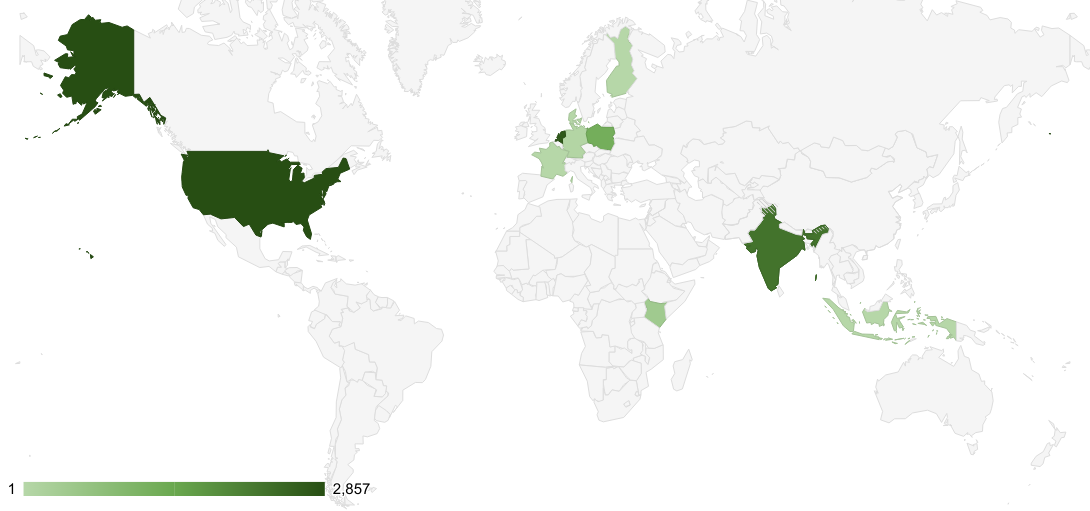
\includegraphics[width=\textwidth]{location-world.png}
	\caption{Usage by Country (Worldwide)}
\end{figure}

\begin{table}[!htb]
	\begin{minipage}{.5\linewidth}
		\caption{Usage by Country}
		\centering
		\begin{tabular}{lr}
			\hline
			\textbf{Country} & \textbf{Pageviews} \\
			\hline
			India            & 986                \\
			The Netherlands  & 666                \\
			Poland           & 237                \\
			Kenya            & 118                \\
			United States    & 109                \\
			United Kingdom   & 92                 \\
			Iran             & 18                 \\
			Indonesia        & 6                  \\
			Germany          & 4                  \\
			Finland          & 4                  \\
			France           & 2                  \\
			Russia           & 2                  \\
			\hline
		\end{tabular}
	\end{minipage}%
	\hspace{.1cm}
	\begin{minipage}{.5\linewidth}
		\centering
		\centering
		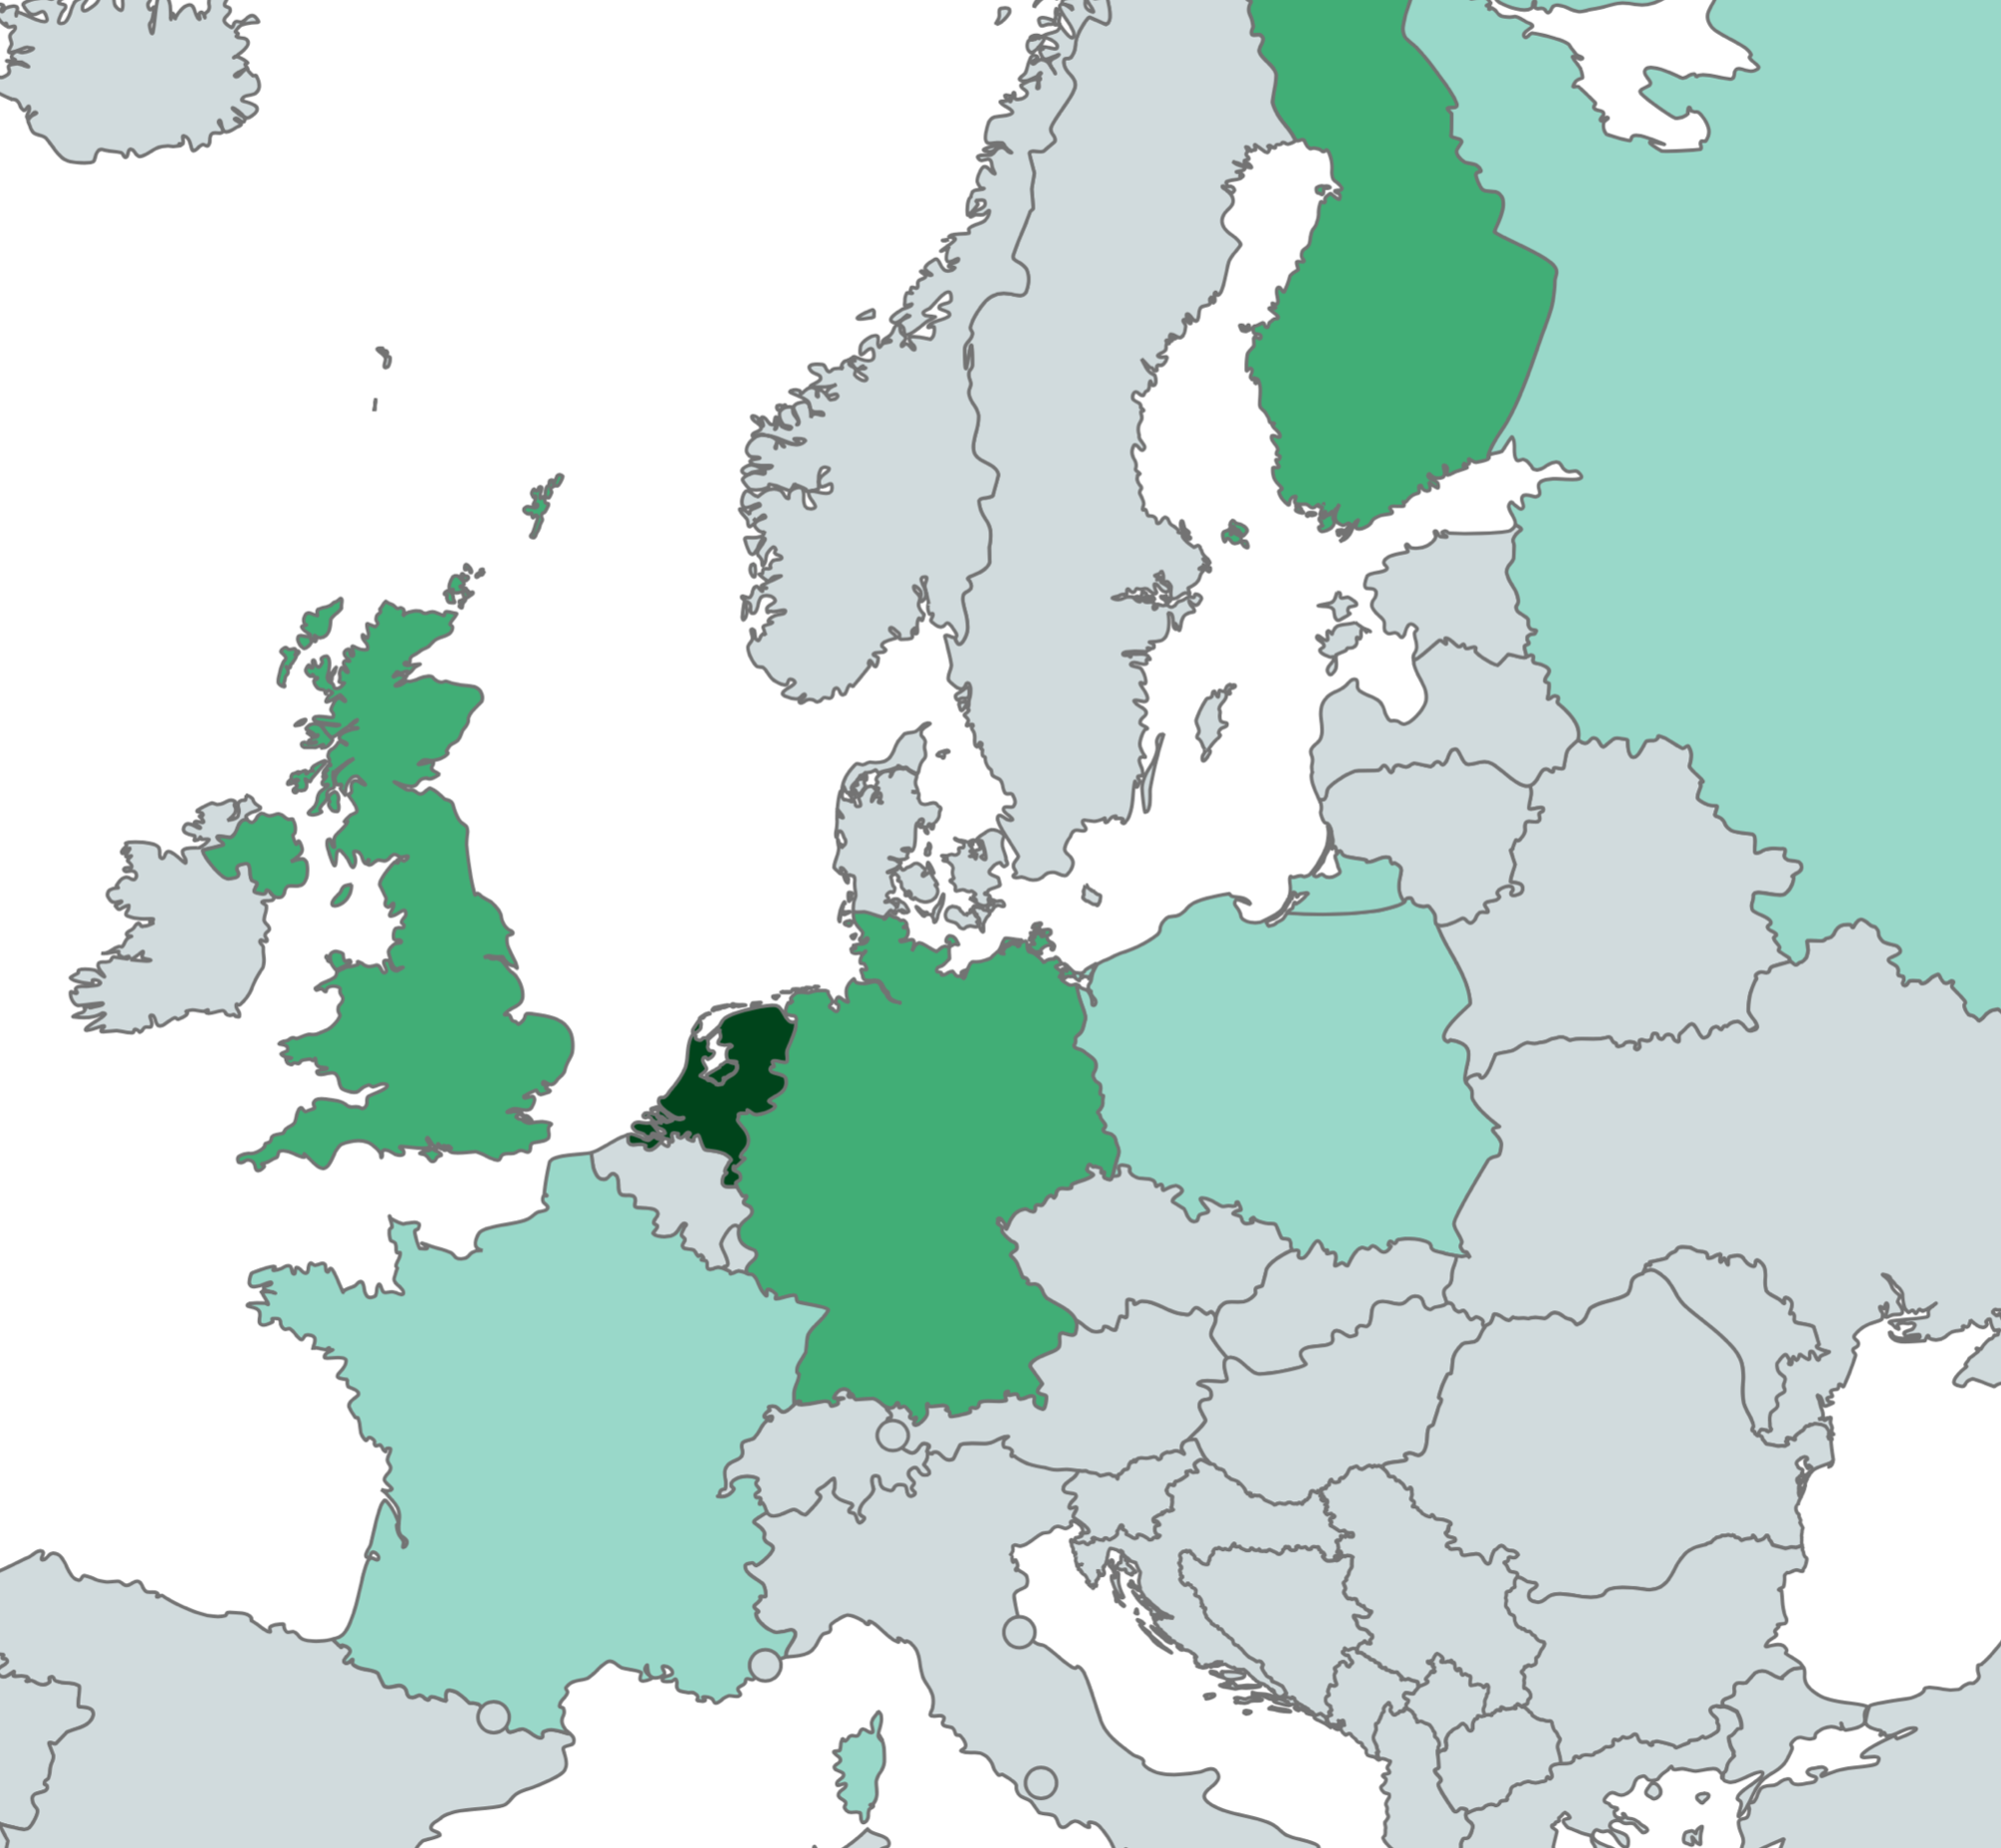
\includegraphics[width=1\linewidth]{location-europe.png}
		\captionof{figure}{Usage by Country (Europe)}
		\label{fig:test2}
	\end{minipage} 
\end{table}

\begin{table}[!htb]
	\begin{minipage}{.5\linewidth}
		\caption{Usage by Dutch Province}
		\centering
		\begin{tabular}{lr}
			\hline
			\textbf{Province} & \textbf{Pageviews} \\
			\hline
			Flevoland         & 363                \\
			Overijssel        & 183                \\
			Gelderland        & 39                 \\
			Utrecht           & 33                 \\
			South Holland     & 18                 \\
			North Holland     & 3                  \\
			Friesland         & 1                  \\
			\hline
		\end{tabular}
	\end{minipage}%
	\hspace{.1cm}
	\begin{minipage}{.5\linewidth}
		\centering
		\centering
		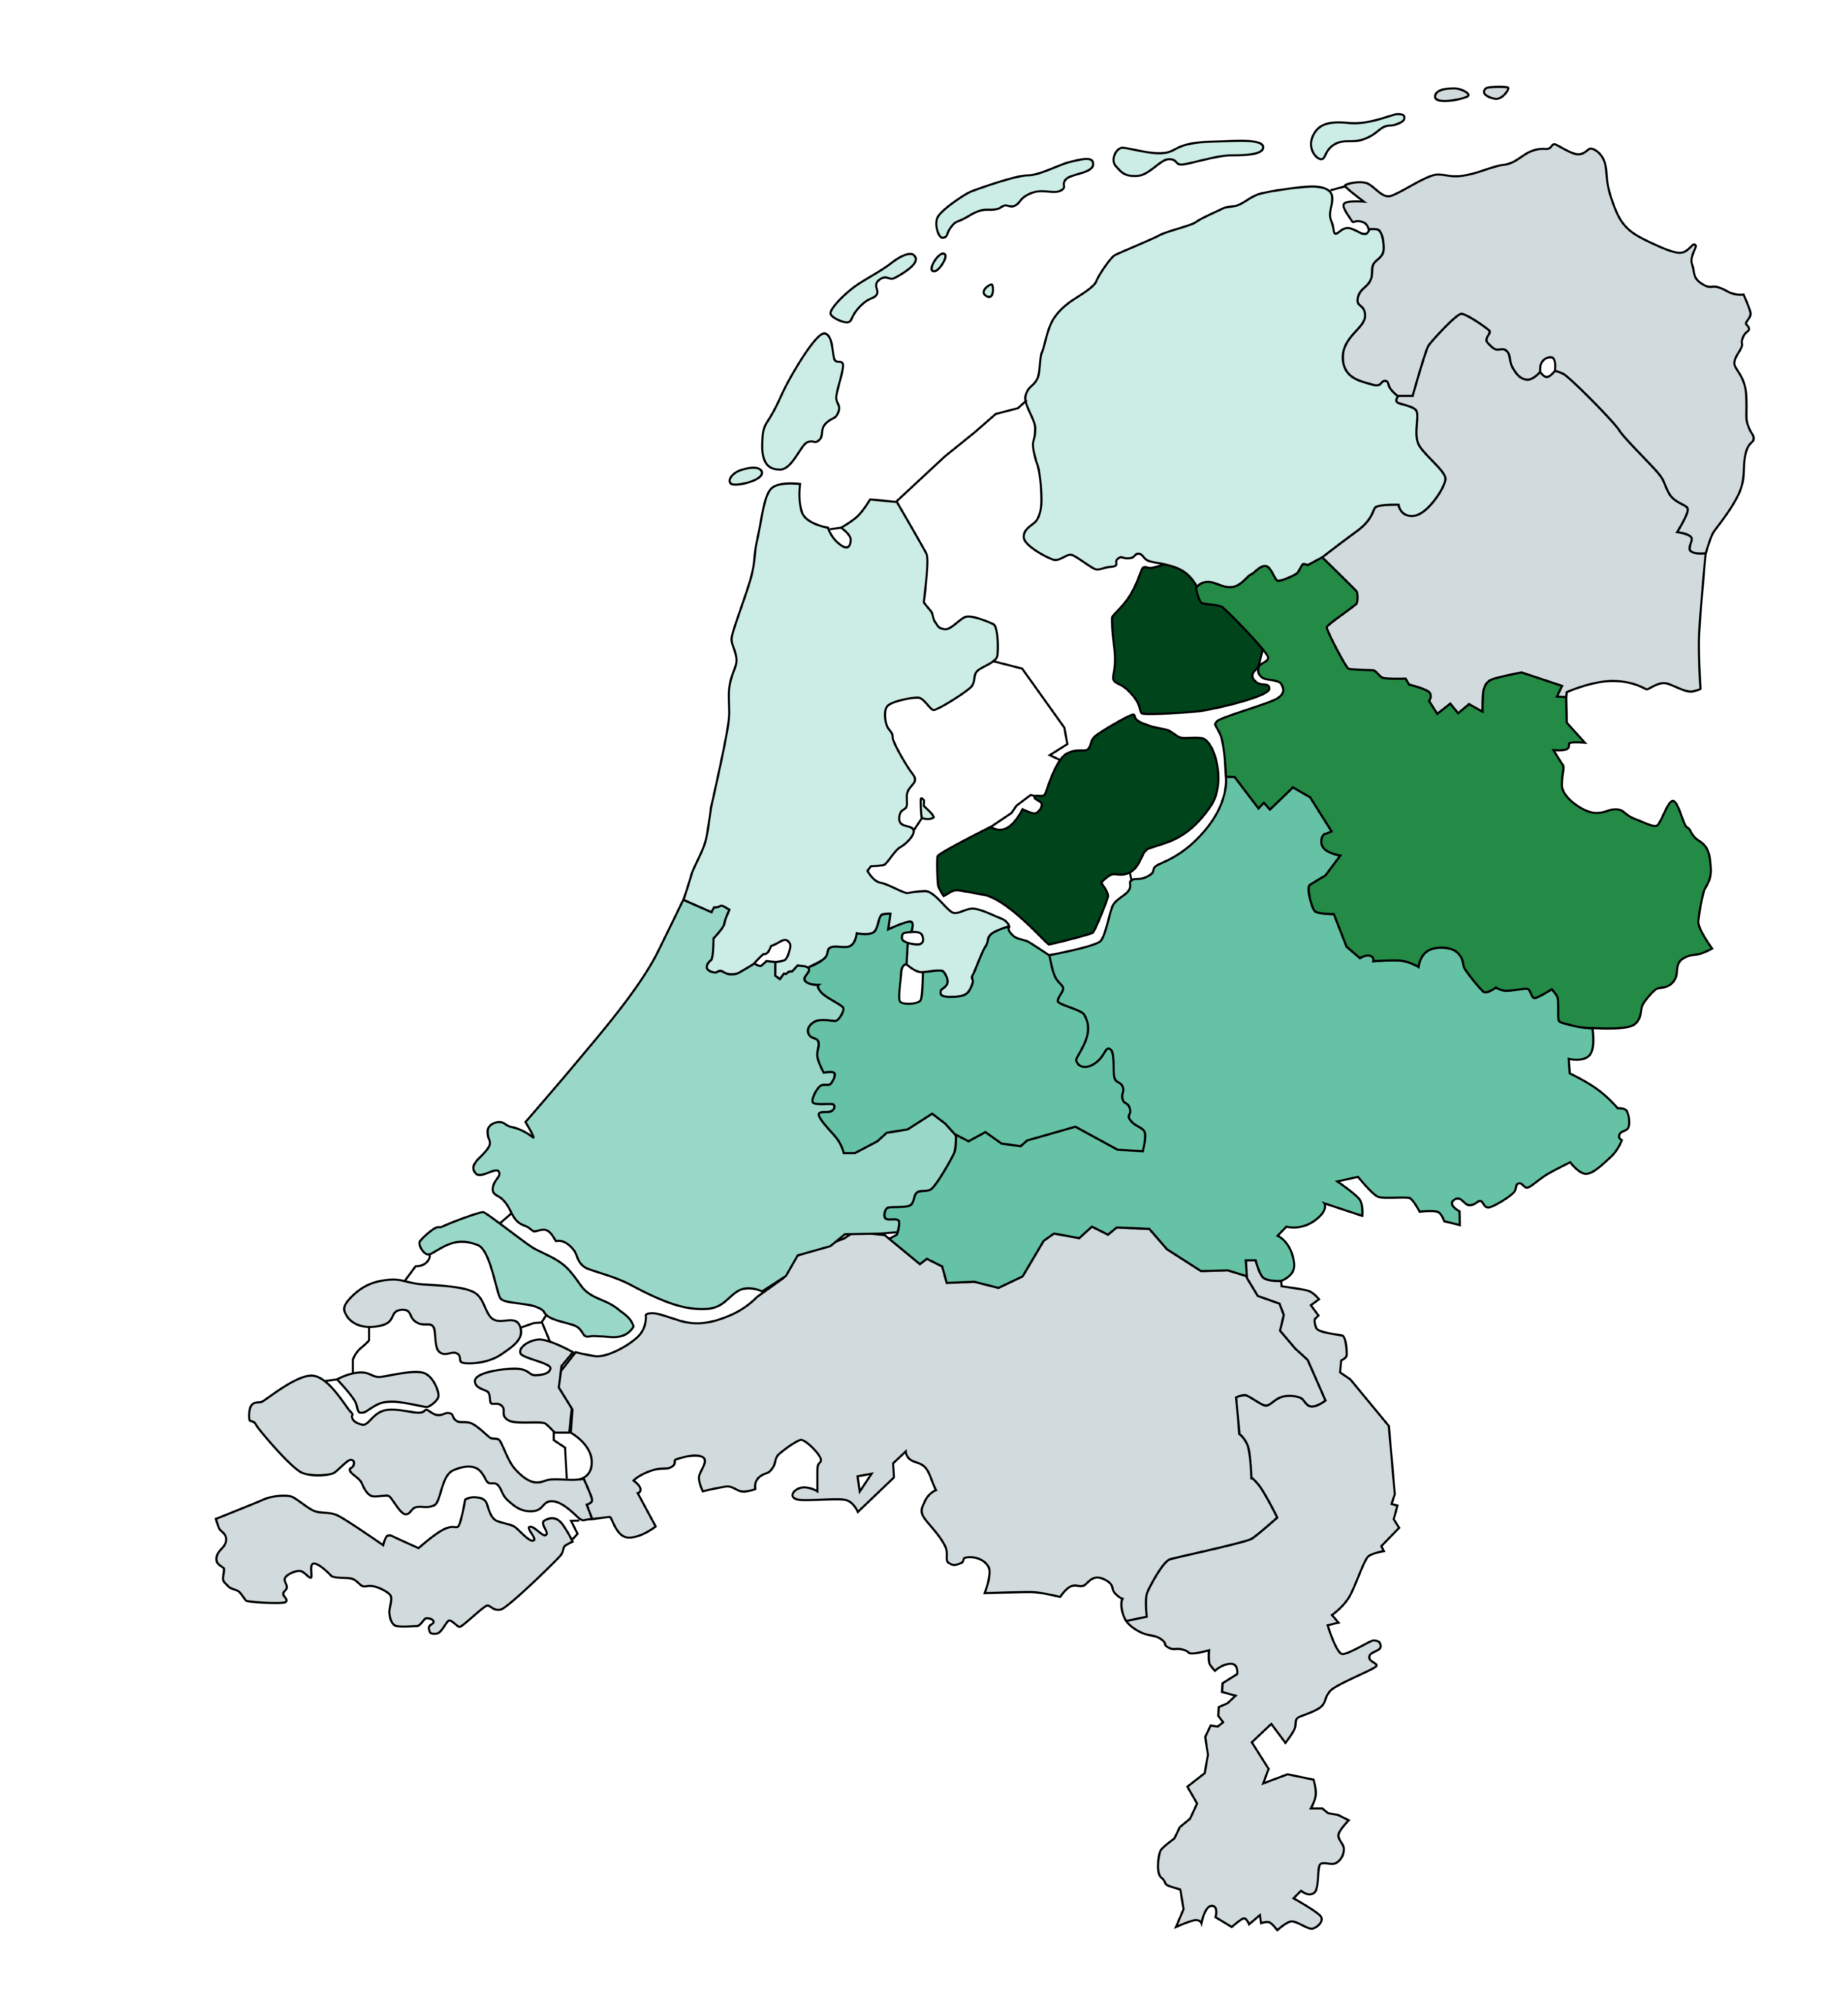
\includegraphics[width=0.66\linewidth]{location-netherlands.png}
		\captionof{figure}{Usage by Dutch Province}
		\label{fig:test2}
	\end{minipage} 
\end{table}

\paragraph{Browsers and Devices} The User-Agent request header is a characteristic string that provides insight into user' browsers and devices, depending on their privacy settings. In Tables 12 and 13, usage by device type and web browser is displayed respectively, with the exception of requests due to uptime monitoring (Section 6.5.1). 

Although Google Chrome is the most popular web browser as reported by Wikimedia in November 2019 \cite{noauthor_dashiki:_nodate}, it placed behind Mozilla Firefox in usage by participants in this research. After Chrome followed Safari, Safari for mobile, and others. `Chrome-releated' is a sum of pageviews from headless Chrome, Chrome webviews, and Chromium.

\begin{table}[!htb]
	\begin{minipage}{.5\linewidth}
		\caption{Usage by Operating System}
		\centering
		\begin{tabular}{lr}
			\hline
			\textbf{Operating System} & \textbf{Pageviews} \\
			\hline
			macOS                     & 992                \\
			Other Linux               & 529                \\
			Windows                   & 377                \\
			Android                   & 217                \\
			iOS                       & 83                 \\
			Ubuntu                    & 44                 \\
			\hline
		\end{tabular}
	\end{minipage}%
	\hspace{.1cm}
	\begin{minipage}{.5\linewidth}
		\centering
		\caption{Usage by Web Browser}
		\begin{tabular}{lr}
			\hline
			\textbf{Browser} & \textbf{Pageviews} \\
			\hline
			Firefox          & 772                \\
			Chrome           & 726                \\
			Safari           & 637                \\
			Safari (mobile)  & 59                 \\
			Chrome-related   & 34                 \\
			Edge             & 3                  \\
			\hline
		\end{tabular}
	\end{minipage} 
\end{table}

\paragraph{Other Analytics}

In terms of the user's browser language, English was the overwhelming majority, detected in all but 35 pageviews. This was divided into 1,311 pageviews in US pageviews, 685 in general English, 206 in British English, and 7 in Indian English. Apart from English, 25 were in Dutch, 8 in Polish, and 2 in Russian. This is positive validation to keep the UI in English.

Similarly, over 99\% of all pageviews were done on URLs on the secure HTTPS protocol, with only 4 requests using HTTP. This was due to the secure protocol redirection described in Section 6.2.5.

Most users used the web app on a large screen, not a smartphone. In fact, over 30 unique screen resolution combinations were tracked. The most common absolute screen resolution was the high definition 1920x1080 (35\%), followed by 1440x900 at almost a quarter of all pageviews. Interestingly, 2\% of all pageviews still used the outdated 800x600 resolution.

\subsubsection{API usage}

Whenever a participant uses the web app, requests to the API are made. An average of 799 API requests were made on each day. The number of requests on each day is graphed in Figure 9, totaling to 19,177.

An API endpoint is triggered when a user sends a new email to their assistant, as described in Section 6.2. Unless an error occurs, the assistant responds to each email as well. Figure 10 shows the number of new emails processed every day. The average number of daily emails processed per day was 7.5 with a total of 98 emails.

\begin{figure}[h]
	\centering
	\begin{minipage}{.47\textwidth}
		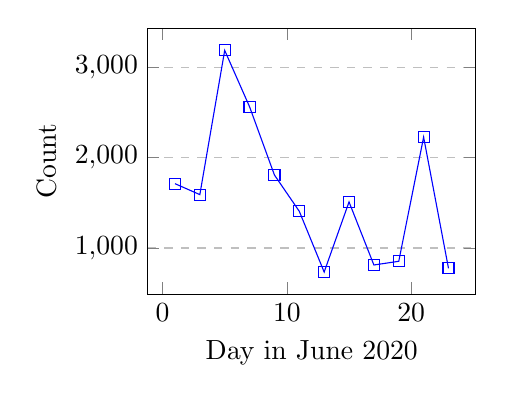
\begin{tikzpicture}
			\begin{axis}[
					width=5.75cm,
					xlabel={Day in June 2020},
					ylabel={Count},
					legend pos=north west,
					ymajorgrids=true,
					grid style=dashed,
				]
				\addplot[
					color=blue,
					mark=square,
				]
				coordinates {
					(1,1712)(3,1591)(5,3187)(7,2563)(9,1808)(11,1406)(13,734)(15,1510)(17,812)(19,853)(21,2227)(23,775)
				};
			\end{axis}
		\end{tikzpicture}
		\caption{Number of API requests received per day}
	\end{minipage}%
	\hspace{.5cm}
	\begin{minipage}{.47\textwidth}
		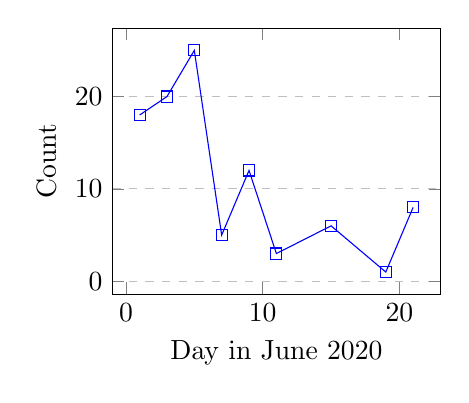
\begin{tikzpicture}
			\begin{axis}[
					width=5.75cm,
					xlabel={Day in June 2020},
					ylabel={Count},
					legend pos=north west,
					ymajorgrids=true,
					grid style=dashed,
				]
				\addplot[
					color=blue,
					mark=square,
				]
				coordinates {
					(1,18)(3,20)(5,25)(7,5)(9,12)(11,3)(15,6)(19,1)(21,8)
				};
				
			\end{axis}
		\end{tikzpicture}
		\caption{Number of emails processed per day}
	\end{minipage}
\end{figure}

\subsubsection{Heatmaps}

To better measure how participants used the web app, each mouse click was also tracked. This tracking was completely anonymous, collecting only the details of the component clicked on apart from the datapoints described above, without linking the clicks to a particular user ID.

Heatmaps convey the distribution of attention on a page \cite{gu_predicting_2020}. A total of 4,940 clicks were tracked and the figures below are presented by superimposing the heatmap over the screenshot of the respective component.

\begin{wrapfigure}{l}{0.45\textwidth}\centering
	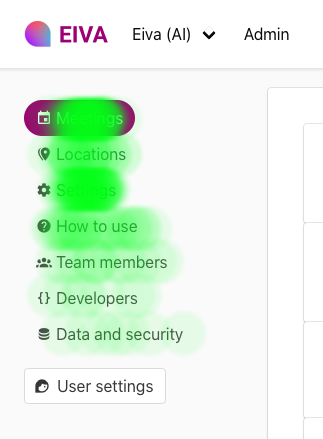
\includegraphics[scale=0.5]{heatmap-sidebar.png}
	\caption{Heatmap for Sidebar}
\end{wrapfigure}

\paragraph{Navigation}

In Figure 11, the distribution of clicks on the sidebar navigation is showcased. This heatmap was generated using 403 datapoints and shows that Settings was clicked on most frequently (106 times), followed in order by Meetings (105), Locations (71), How to use (58), Team members (13), Developers (20), and Data and security (15).

\begin{figure}[h]
	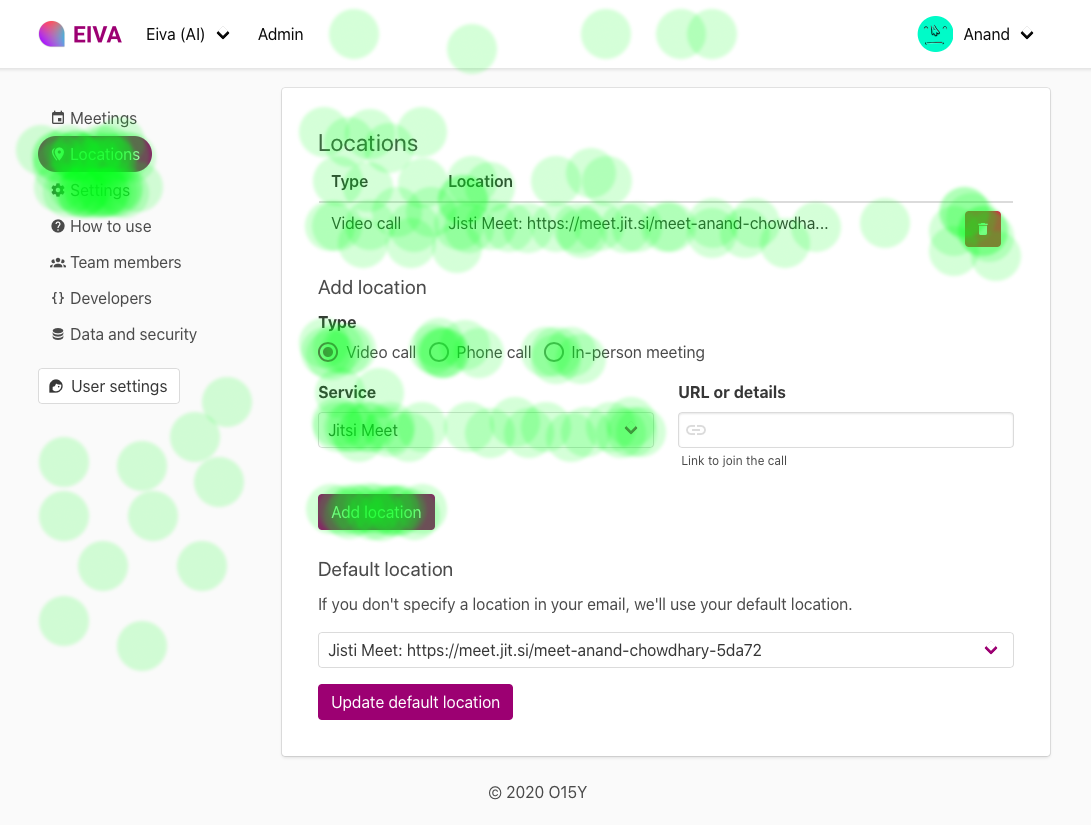
\includegraphics[width=\textwidth]{heatmap-locations.png}
	\caption{Heatmap for Locations Page}
\end{figure}

\paragraph{Webpage}

The Locations page is an ideal example to measure clicks because it has several controls and links. Figure 12, generated with 237 datapoints, shows.

The sidebar navigation on the Locations page has the most frequently clicked item of Settings (19 clicks), which is expected since it is the next link after Locations itself. Users also clicked on the table containing the list of saved locations and the Delete button for each item.

In the Add Locations selector, both Video call and Phone call were selected 6 times, whereas In-person meeting was selected 5 times. The Service dropdown selector was clicked on 24 times. The Add Location button was clicked on 14 times. In this example, the Update default location button in unused because it was added after June 10, 2020.

Overall, it is clear that users interacted with all controls on the webpage --- the sidebar navigation, locations table, buttons, and input fields.

\subsection{User Experience Evaluation}

The first question, \emph{What comes to mind when you think about EIVA; how would you describe it to a friend?}, allows users to share their first impressions after using the service. Some of the responses were:

\begin{enumerate}
	\item ``A smart interface to my calendar"
	\item ``A way to avoid having to talk to people to schedule your appointments with them"
	\item ``Make my appointment very easy, Easy to see all meetings in one screen! Awesome Product!"
	\item ``Interesting personal automation, severely limited at the moment"
\end{enumerate}

\subsubsection{Webapp Experience}

Users were asked to rate the web app on different parameters, from 0 to 5. All parameters scored over 4 out of 5, with privacy features rated with the highest average of 4.7.

\begin{table}[!htb]
	\begin{minipage}{1\linewidth}
		\caption{Webapp Experience Ratings}
		\centering
		\begin{tabular}{llcc}
			\hline
			\textbf{Parameter} & \textbf{Average}   & \textbf{Median} & \textbf{Mode} \\
			\hline
			Overall experience & \score{4.4}{5} 4.4 & 5               & 5             \\
			Design             & \score{4.6}{5} 4.6 & 5               & 5             \\
			Functionality      & \score{4.5}{5} 4.5 & 5               & 5             \\
			Ease of use        & \score{4.4}{5} 4.4 & 4.5             & 5             \\
			Privacy features   & \score{4.7}{5} 4.7 & 5               & 5             \\
			Onboarding flow    & \score{4.5}{5} 4.5 & 5               & 5             \\
			Introductory tour  & \score{4.2}{5} 4.2 & 4               & 5             \\
			\hline
		\end{tabular}
	\end{minipage}%
\end{table}

\subsubsection{Assistant Experience}

Similarly, users were asked to rate the assistant on different parameters, from 0 to 5. All but two parameters scored an average greater than 4, with the lowest-rated question being \emph{How much do you trust the assistant to not make mistakes?}. Participants rated the overall experience as 4.5 out of 5, and customizability and flexibility as 4.4 each.

\begin{table}[!htb]
	\begin{minipage}{1\linewidth}
		\caption{Assistant Experience Ratings}
		\centering
		\begin{tabular}{llcc}
			\hline
			\textbf{Parameter}                    & \textbf{Average}   & \textbf{Median} & \textbf{Mode} \\
			\hline
			Overall experience                    & \score{4.5}{5} 4.5 & 5               & 5             \\
			Customizability                       & \score{4.4}{5} 4.4 & 5               & 5             \\
			Flexibility in understanding language & \score{4.4}{5} 4.4 & 5               & 5             \\
			Sounding human-like over email        & \score{4.1}{5} 4.1 & 4               & 5             \\
			Trust to not make mistakes            & \score{3.6}{5} 3.6 & 4               & 4             \\
			Time recommendation accuracy          & \score{3.9}{5} 3.9 & 4               & 4             \\
			\hline
		\end{tabular}
	\end{minipage}%
\end{table}

To participate in the research, users were required to send at least one email to the EIVA for scheduling an appointment. They were free to send multiple emails, and were asked about the number of emails they sent. 10 out of 30 participants sent between 2 and 5 emails, while the other 20 only sent the one.

To find out whether the assistant understood the overall meaning of their email in natural language, participants were asked \emph{Did the assistant understand your email(s) correctly?}. 24 out of 30 participants responded in the affirmative and 5 out of 10 responded with `Partially', while only one participant responded in the negative. This suggests that the EIVA did a well-enough job understanding incoming emails most of the time.

\begin{table}[!htb]
	\begin{minipage}{.5\linewidth}
		\caption{Number of Emails Sent}
		\centering
		\begin{tabular}{lr}
			\hline
			\textbf{Number} & \textbf{Count} \\
			\hline
			1               & 20             \\
			Between 2 and 5 & 10             \\
			More than 5     & 0              \\
			\hline
		\end{tabular}
	\end{minipage}%
	\hspace{.1cm}
	\begin{minipage}{.5\linewidth}
		\centering
		\caption{Correctly Understood}
		\begin{tabular}{lr}
			\hline
			\textbf{Response} & \textbf{Count} \\
			\hline
			Yes               & 24             \\
			Partially         & 5              \\
			No                & 1              \\
			\hline
		\end{tabular}
	\end{minipage} 
\end{table}

Apart from understanding the meaning of an email, participants were asked whether the EIVA recommended the correct location for the meeting. The location recommendation was correct for 24 out of 30 participants and incorrect for 5 participants. 1 participant chose to not answer this question.

Because of the API webhook, EIVA responds to emails almost instantly. When asked about whether the assistant responded to emails in a reasonable amount of time, all 30 participants responded with `Yes'.

They were also directly asked whether the EIVA met their expectation in terms of scheduling an appointment. All but one participants responded positively.

\begin{table}[!htb]
	\begin{minipage}{.5\linewidth}
		\caption{Location Recommendation}
		\centering
		\begin{tabular}{lr}
			\hline
			\textbf{Accurate} & \textbf{Count} \\
			\hline
			Correct           & 24             \\
			Incorrect         & 5              \\
			\hline
		\end{tabular}
	\end{minipage}%
	\hspace{.1cm}
	\begin{minipage}{.5\linewidth}
		\centering
		\caption{EIVA Met Expectations}
		\begin{tabular}{lr}
			\hline
			\textbf{Response} & \textbf{Count} \\
			\hline
			Yes               & 29             \\
			No                & 1              \\
			\hline
		\end{tabular}
	\end{minipage} 
\end{table}

To test the hypothesis proposed in Section 4.2.1, users were asked \emph{If you were the recipient of an email from EIVA, would you be able to tell whether it's an email from an AI or human assistant, if you didn't already know?}. Table 23 shows that 11 out of 30 participants said that they would be able to tell, while 18 out of 30 said that they wouldn't. 1 participants chose to not answer.

\subsubsection{Business Case}

Since the big picture goal of the client is to launch EIVA as a paid service, participants were asked whether they would use EIVA on launch. 25 out of 30 participants said that they would, whereas 5 said that they wouldn't.

Participants were also asked how much they would be willing to pay every month for such as service. 6 out of 30 participants said that the service should be free, 13 out of 30 would be willing to pay up to €5 per month, while 10 out of 30 would pay up to €10 per month. One participant wanted to pay €20 or more per month.

Although it seems like the average amount users would want to pay is up to €6.16 per month, this includes all professional categories of respondents. Calculating individually, the average for students is up to €4.44 per month, for employees of a company or organization, it is up to €6.38 per month; and for self-employed professionals or freelancers, it is as high as €10 per month.

\begin{table}[!htb]
	\begin{minipage}{.5\linewidth}
		\caption{Would Use EIVA}
		\centering
		\begin{tabular}{lr}
			\hline
			\textbf{Accurate} & \textbf{Count} \\
			\hline
			Yes               & 25             \\
			No                & 5              \\
			\hline
		\end{tabular}
	\end{minipage}%
	\hspace{.1cm}
	\begin{minipage}{.5\linewidth}
		\centering
		\caption{Monthly Subscription Fees}
		\begin{tabular}{lr}
			\hline
			\textbf{Response} & \textbf{Count} \\
			\hline
			€0              & 6              \\
			€5 or less      & 13             \\
			€10 or less     & 10             \\
			€20 or less     & 0              \\
			More than €20   & 1              \\
			\hline
		\end{tabular}
	\end{minipage}
\end{table}

\subsubsection{Final Impressions}

Respondents could optionally add additional information in the form of long-form answers. A selection of answers with analysis is listed below, and all answers are available in Appendix 1.

When asked \emph{What do you like the most about EIVA?}, 5 users mentioned the ease of use and 3 users mentioned the fast response time. User also liked the overall concept, security features, and the fact that EIVA doesn't interfere with their normal workflow and users don't have to manually select time slots. They also liked the natural-language conversation and the user interface. Some quotes are ``[EIVA is] easy to handle and helps you to save your time and energy," and ``[EIVA] takes the most painstaking part of the workhours off [your] hands".

On the contrary, responses to the question \emph{What do you like the least about EIVA?} included ``pretending to be human", the ``lengthy and slightly technical" onboarding process, and the mobile interface. One user also said that ``[EIVA] doesn't fully seem to know/understand my reasoning behind picking or proposing certain meeting times, where maintaining focus during my work day plays an important role." This suggests that more fine-grained control over recommended time slots should be allowed in the web app interface.

Tables 24 and 25 analyze responses to questions \emph{Did you find anything frustrating that you wish was easier or different?} and \emph{Is there anything that you wish the assistant could do, in terms of scheduling, that it doesn't currently?} respectively.

Lastly, users had the option of adding any additional feedback, suggestions, or comments, which almost half of all respondents chose to add. One user said ``I really EIVA, and I think that we need such kind of smart applications in today's world that do not only save time, but also help us act more efficiently in other work as well." Users also stated that EIVA is ``great and extremely easy to use" and has ``great potential".

\begin{table}[!htb]
	\caption{User Frustrations}
	\centering
	\begin{tabular}{p{4cm}p{7cm}}
		\hline
		\textbf{Response}                                   & \textbf{Analysis}                                                                                                                                                    \\
		\hline
		Dutch grammar can be improved                       & As a non-native speaker, Google Translate was used for Dutch text in emails                                                                                          \\
		\hline
		Onboarding is too long or should be skippable       & The current onboarding flow takes users through each setting and page; this was to ensure users know of all available options, but can be understandably frustrating \\
		\hline
		Time recommendations should take email into account & EIVA initially recommended there time slots in the following week, but has since improved to understand email content and recommend accordingly                      \\
		\hline
		Onboarding starts again on second log in            & The onboarding completion status is stored in local storage, so logging in from another device will ask users to complete the tour again                             \\
		\hline
		Adding calendar connection URL is hard              & Users have to know how to generate an iCalendar URL from their calendar client of choice, so documentation should be added to make that process simpler              \\
		\hline
		Slow activation email                               & The cron to send emails is scheduled for every minute, so it can take up to 60 seconds to send an email to users                                                     \\
		\hline
	\end{tabular}
\end{table}

\begin{table}[!htb]
	\caption{Feature Recommendations}
	\centering
	\begin{tabular}{p{4cm}p{7cm}}
		\hline
		\textbf{Recommendation}                          & \textbf{Analysis}                                                                                        \\
		\hline
		Create a meeting without having to send an email & The web app can include an option to manually schedule meetings                                          \\
		\hline
		Support SMS or WhatsApp instead of email         & Currently, EIVA only works over email, and more form factors can be added over time                      \\
		\hline
		Send daily schedule summary emails               & This was a feature part of Ideation, but was not implemented due to time constraints and should be added \\
		\hline
		Invite multiple guests in each appointment       & Users can already invite multiple guests, but slot selection UI has to be improved                       \\
		\hline
		Select preferred meeting time slots manually     & This can be added by providing a preference UI for each slot                                             \\
		\hline
		Increase number of recommended daily slots       & A customizable setting can be added with the number of recommendations to send                           \\
		\hline
		Cancel or reschedule meetings from the web app   & This was another feature part of Ideation that wasn't implemented and should be added                    \\
		\hline
	\end{tabular}
\end{table}

\newpage

\section{Conclusion}

A functional Email-based Intelligent Virtual Assistant (EIVA) was developed along with its companion web app using TypeScript with Node.js and Vue.js, and with a focus on industry best-practices and customizability.

30 users from around the world participated in this research, with a majority coming from India and the Netherlands. Most participants were employed full-time, many were students, and some were freelancers. The hypothesis that email is the most common mode for scheduling appointments was supported by the results of the Introductory Survey. Participants used a variety of devices, operating systems, and web browsers to use the web app, and sent almost 100 total emails to their assistants. 19,177 API requests from 2,244 pageviews were tracked, and heatmaps for mouse clicks were also generated to measure the distribution of attention on webpages.

Participants responded very positively after using the assistant and the web app, with overall experience ratings of 4.5 and 4.4 out of 5 respectively. The privacy features were most highly rated (4.7), and users also enjoyed the design of the interface (4.6), the onboarding flow (4.5), and the ease-of-use (4.4). Flexibility in understanding natural language was rated 4.4 and sounding human-like over email was rated 4.1. The lowest ratings were for time recommendation accuracy (3.9) and trust not to make mistakes (3.6).  This suggests that users are excited about the product, but there is still work to be done to increase the assistant's utility. Respondents also shared their frustrations and recommendations, which were analyzed for future work.

All but one participants said that the EIVA met their expectations, and 25 out of 30 would use it in the future if it launches as a service. Most would also be willing to pay for it, with an average amount up to €6.16 per month.

\newpage

\section{Future Work}

\subsection{Features and Improvements}

In Section 7.3.4, participants shared their frustrations which included enhancements and bugs, which should be fixed. For example, Dutch grammar should be improved with the help of a native speaker, onboarding time should be reduced, documentation should be improved, and time recommendations should be smarter and context-aware.

Users also shared feature recommendations which should be implemented in the future. New features such as setting up appointment without sending emails and support for other forms of communication like instant messages and SMS should also be added. Users can also currently not able to manually select recommended slots, or cancel or reschedule meetings. Furthermore, support for multiple guests also needs several improvements.

In terms of technical updates, a bloom filter may be used when searching for invalidated tokens, which will make the search faster and more efficient on scale. Prisma, the database toolkit used by the backend, also recently added support for native JSON data types, so the dependencies and source code should be updated with the new syntax. The NLP training data can also be increased to add support for more languages.

\subsection{Business Case}

In Section 2, it is highlighted that professionals currently either schedule appointments themselves or hire assistants to help with the task. However, regardless of whether the professional or their assistant schedules appointments, the time wasted is not insignificant. According to the European Commission, the average Dutch small or medium-sized enterprise (SME) employs 3.2 people \cite{noauthor_2019_2019}. If each employee attends 7 meetings per week (which is the average for professionals), 26 otherwise productive hours are wasted every month in scheduling meetings \cite{kincaid_electronic_1985}. This costs the company over €450 in lost time, based on the average wage of €17.6 per hour \cite{wedia_salary_nodate} This adds up to almost €2.25 billion per year for the SME industry as a whole, and the numbers are even higher for larger enterprises. University of Twente, for example, employs 3,150 professionals, adding up to over €400,000 in lost time per year.

Therefore, a strong business case can be built around launching EIVA as a service. Since the assistant can save around €150 in lost time per month for professionals, a service that costs as high as €100 per month per person has a return on investment (ROI) of 50\%. That being said, a pricing point of less than €50 per month can be achieved because of the low cloud infrastructure costs. The proposed pricing plans are:

\begin{enumerate}
	\item Basic plan for €10 per month, targeted towards students, self-employed young professionals, and early-stage entrepreneurs. This plan will have no support for custom domain names, but will include unlimited scheduling and assistant usage.
	\item Pro plan for €25 per month. This will include all features of the Basic plan with support for custom domain names.
	\item Team plan for €30 per user per month, targeted towards businesses or institutions who want to onboard their entire team to EIVA for a collaborative experience.
	\item Custom plan with custom billing for large enterprises with features like dedicated support, on-premise hosting, and uptime service-level agreements (SLA).
\end{enumerate}

\subsection{Impact Assessment}

When deploying this service to the market, there can be several ethical and societal challenges that need to be explored, such as AI-driven job loss. Therefore, an impact assessment must be conducted before launch.

Just like in other applications of automation software, loss of employment for assistants is an important social disruption that this product unfortunately encourages. In the interest of saving both time and money, companies may choose to deploy AI-powered assistants on an organization-wide level and terminate the employment of all their secretaries in the future.

In a survey of administrative assistants, all but one reported that most of their work was scheduling-related \cite{erickson_assistance:_2008}. Though in the current state, EIVA only focuses on appointment scheduling, this is expected to change in the future as more features are added. Slowly, software agents like EIVA will be able to do more and more of the day-to-day job of an assistant, and will prove to be both faster and more inexpensive.

For the purposes of this thesis project, there is a strong conclusion that as EIVAs become smarter and market adoption increases, there definitely will be a cause-effect relationship with human assistant unemployment. I'd further say that someone who has used an EVA (and perhaps paid around \$20 per month for it) will not ever want to go back to a human assistant that is slower, makes more mistakes, and costs over 100x more.

\newpage

\cleardoublepage
\pagenumbering{roman}
\setcounter{page}{\thesavepage}

\section*{Appendix 1: Information Brochure}

If you want to get in touch with the researchers, client, or supervisor, you can find their details below. If you have any queries, complaints, or comments about this research, you can contact the Secretary of the Ethics Committee.

\paragraph{Research Leader}
Anand Chowdhary\newline
Address: Roerstaart 28, 7543AC Enschede, the Netherlands\newline
Phone: +31 0 644691056\newline
Email: a.chowdhary@student.utwente.nl

\paragraph{Research Client}
Speakup B.V.\newline
Address: Institutenweg 6, 7521PK Enschede, the Netherlands\newline
Phone: +31 0 887732587\newline
Email: info@speakup.nl

\paragraph{Research Supervisor}
Dr. Job Zwiers\newline
Address: Zilverling 1060, 7522NH Enschede, the Netherlands\newline
Phone: +31 0 534893816\newline
Email: j.zwiers@utwente.nl

\paragraph{Secretary of the Ethics Committee}
Dr. Petri de Willigen\newline
Address: Zilverling 1051, 7522NH Enschede, the Netherlands\newline
Phone: +31 0 534892085\newline
Email: ethics-comm-ewi@utwente.nl

\paragraph{Purpose}

Scheduling appointments manually can waste a lot of time, and our goal is to provide you with a virtual assistant that can automate the process of scheduling based on your preferences and availability. This research will help us understand the accuracy of the assistant, the end user experience, and whether or not end users will use it when we launch it as a service.

\paragraph{Research Procedure}

After you have signed the Consent Form and answered some questions, you can register for the virtual assistant service on the website. An onboarding interface will help you set up your account, connect your calendar, and set up your scheduling preferences (such as working days, meeting locations, and preferred times). After using the virtual assistant to schedule at least one meeting, you can continue to fill this survey about your experience. Apart from your survey response, computed data such as how long it takes the assistant to set up your appointment and analytics about your usage of the web application will also be collected and aggregated. Once the research is over, you can choose to receive a copy of the results.

\paragraph{10 Minutes}

It will takes around 10 minutes to complete this survey, including interacting with your virtual assistant. It is recommended to use a laptop, tablet, or desktop computer. If none of these are available to you, you can also use a smartphone. After you have submitted this form, you can continue to use the virtual assistant service, if you choose to, but only the usage within the research period will be measured.

\paragraph{Remuneration}

This research is voluntary and there is no monetary compensation for participation. However, after this research has ended, this virtual assistant service will launch as a paid subscription service for professionals. As a research participant, you will receive €100 in service credits or equivalent, and a coupon code will be emailed to you at the end of this research.

\paragraph{Anonymous}

Anonymity will be guaranteed to all participants, and your individual data will not be disclosed to third parties without your explicit permission. Furthermore, the data obtained from this research is not published in any way that would make it possible to link the results or other findings with a particular subject. Only aggregated or anonymized data will be published.

\paragraph{Voluntary}

Participation remains at all times voluntary and you may refuse to participate in this research at any time, without giving any reason. You can also refuse that we use your data for the research within 24 hours of completing the survey. There is no specific category of persons who are advised not to participate in the research due to an increased level of risk or discomfort.

\paragraph{COVID-19 Note}

This research is completely online and based on your usage of a web application, sending emails, and answering a survey. At no point will participants be asked to interact with a physical installation or answer questions in person. It is recommended that you participate from the comfort of your home. There is no possibility of accidental discoveries in this research.

\newpage

\section*{Appendix 2: Consent Form}

This section ensures that we have your permission to conduct this research. Please note that participation remains at all times voluntary and you may refuse to participate in this research at any time, without giving any reason.

\begin{enumerate}
	\item Before we sign you up for this research, we need to make sure that you can give us permission. Note that you are not eligible for this research if you are under the age of 18 or otherwise incapable of giving us your informed consent. I am above the age of 18 and capable of giving informed consent.
	\item In this research, you will use a virtual assistant web application and communicate with the assistant over email. You will have to answer a series of questions about your experience using the application and communicating with the assistant. By checking ``I agree", you permit us to use the data from your answers for purposes of this research.
	\item Optional: To find available meeting slots in your agenda, the virtual assistant will require access to your calendar. To allow access, you can add a link to your calendar using the web app. You can also remove access at any time. By checking ``I agree", you permit us to have read-only access to your calendar.
	\item In order to use the web application, you provide your personal information such as your name and email address. Optionally, you can also add your phone numbers and office addresses to allow the virtual assistant to schedule in-person meetings or phone calls. By checking ``I agree", you permit us to store this information and use it for scheduling appointments.
	\item Your usage of the web application will be analyzed in the background, such as how long it takes you to complete the onboarding flow and to set up an appointment using the assistant. This data will be only be collected anonymously and published after aggregation. By checking ``I agree", you permit this data collection.
	\item Under the General Data Protection Regulation, we need your permission to store your information on our servers. You can export a copy of all your data or permanently delete it at any time from the web application. By selecting an option, you permit us to store your information.
\end{enumerate}

\newpage

\section*{Appendix 3: Raw Responses}

All raw responses from the survey are available in CSV format on the GitHub project: \url{https://github.com/AnandChowdhary/bsc-thesis} in \texttt{responses.csv}.

The following table shows all collected responses for rating questions. Columns refer to question number while rows are randomized responses. In the last three rows, $\bar{x}$ refers to the sample mean, $\tilde{x}$ is the median, and $Mo$ is the mode.

\begin{table}[!htb]
	\begin{minipage}{1\linewidth}
		\caption{All Raw Responses to Rating Questions}
		\centering
		\begin{tabular}{|*{13}{p{0.5cm}|}}
			\hline
			            & \textbf{1}   & \textbf{2}   & \textbf{3}   & \textbf{4}   & \textbf{5}   & \textbf{6}   & \textbf{7}   & \textbf{8}   & \textbf{9}   & \textbf{10}  & \textbf{11}  & \textbf{12}  \\
			\hline
			\textbf{1}  & 5            & 5            & 5            & 5            & 5            & 5            & 5            & 5            & 5            & 5            & 5            & 5            \\
			\textbf{2}  & 4            & 4            & 4            & 3            & 5            & 5            & 3            & 4            & 3            & 3            & 4            & 3            \\
			\textbf{3}  & 4            & 4            & 4            & 4            & 5            & 4            & 1            & 4            & 4            & 2            & 3            & 4            \\
			\textbf{4}  & 5            & 5            & 5            & 4            & 5            & 5            & 3            & 5            & 5            & 5            & 3            & 4            \\
			\textbf{5}  & 5            & 5            & 5            & 5            & 5            & 5            & 5            & 5            & 5            & 5            & 3            & 1            \\
			\textbf{6}  & 3            & 5            & 4            & 4            & 4            & 4            & 4            & 4            & 4            & 4            & 4            & 4            \\
			\textbf{7}  & 5            & 5            & 5            & 5            & 5            & 5            & 5            & 5            & 5            & 5            & 5            & 5            \\
			\textbf{8}  & 5            & 5            & 5            & 5            & 5            & 5            & 4            & 5            & 5            & 5            & 5            & 4            \\
			\textbf{9}  & 4            & 4            & 4            & 3            & 4            & 3            & 4            & 4            & 5            & 4            & 4            & 3            \\
			\textbf{10} & 3            & 4            & 3            & 3            & 3            & 3            & 3            & 1            & 2            & 2            & 2            & 2            \\
			\textbf{11} & 5            & 5            & 5            & 4            & 5            & 4            & 4            & 5            & 5            & 4            & 4            & 4            \\
			\textbf{12} & 4            & 5            & 4            & 3            & 4            & 4            & 5            & 5            & 4            & 4            & 4            & 3            \\
			\textbf{13} & 4            & 5            & 4            & 4            & 4            & 4            & 4            & 4            & 3            & 3            & 3            & 2            \\
			\textbf{14} & 5            & 5            & 5            & 5            & 5            & 4            & 5            & 5            & 5            & 5            & 5            & 5            \\
			\textbf{15} & 5            & 5            & 5            & 5            & 5            & 5            & 5            & 5            & 5            & 5            & 5            & 5            \\
			\textbf{16} & 5            & 5            & 5            & 5            & 5            & 5            & 5            & 5            & 5            & 5            & 5            & 5            \\
			\textbf{17} & 5            & 5            & 5            & 5            & 5            & 5            & 5            & 5            & 5            & 5            & 5            & 5            \\
			\textbf{18} & 5            & 5            & 5            & 5            & 5            & 5            & 5            & 5            & 5            & 5            & 3            & 1            \\
			\textbf{19} & 5            & 4            & 5            & 5            & 4            & 5            & 5            & 5            & 4            & 5            & 5            & 3            \\
			\textbf{20} & 4            & 5            & 4            & 4            & 4            & 5            & 4            & 5            & 4            & 5            & 4            & 4            \\
			\textbf{21} & 4            & 5            & 4            & 5            & 5            & 5            & 5            & 4            & 5            & 5            & 5            & 3            \\
			\textbf{22} & 5            & 5            & 4            & 5            & 5            & 5            & 5            & 5            & 4            & 5            & 4            & 3            \\
			\textbf{23} & 3            & 2            & 4            & 5            & 5            & 5            & 5            & 5            & 5            & 5            & 5            & 4            \\
			\textbf{24} & 4            & 4            & 4            & 4            & 4            & 3            & 4            & 4            & 3            & 4            & 4            & 3            \\
			\textbf{25} & 5            & 5            & 5            & 4            & 5            & 5            & 3            & 5            & 4            & 4            & 3            & 5            \\
			\textbf{26} & 3            & 4            & 4            & 4            & 4            & 4            & 3            & 4            & 4            & 4            & 4            & 4            \\
			\textbf{27} & 4            & 4            & 5            & 5            & 5            & 5            & 4            & 5            & 5            & 4            & 4            & 3            \\
			\textbf{28} & 4            & 5            & 4            & 4            & 5            & 5            & 4            & 4            & 4            & 4            & 4            & 4            \\
			\textbf{29} & 5            & 5            & 5            & 4            & 5            & 4            & 3            & 5            & 5            & 5            & 5            & 4            \\
			\textbf{30} & 5            & 4            & 5            & 5            & 5            & 5            & 5            & 3            & 5            & 5            & 3            & 2            \\
			$\bar{x}$   & \textbf{4.4} & \textbf{4.6} & \textbf{4.5} & \textbf{4.4} & \textbf{4.7} & \textbf{4.5} & \textbf{4.2} & \textbf{4.5} & \textbf{4.4} & \textbf{4.4} & \textbf{4.1} & \textbf{3.6} \\
			$\tilde{x}$ & 5            & 5            & 5            & 4.5          & 5            & 5            & 4            & 5            & 5            & 5            & 4            & 4            \\
			$Mo$        & 5            & 5            & 5            & 5            & 5            & 5            & 5            & 5            & 5            & 5            & 5            & 4            \\
			\hline
		\end{tabular}
	\end{minipage}%
\end{table}

\newpage

\section*{Appendix 4: Code Repositories}

All code written for this project is open source, available on GitHub:

\begin{enumerate}
	\item Backend APIs: \url{https://github.com/o15y/eiva}
	\item Frontend web application: \url{https://github.com/o15y/myeiva.com}
	\item Thesis: \url{https://github.com/AnandChowdhary/bsc-thesis}
	\item Companion open source packages:
	      \begin{enumerate}
	      	\item Calendar Slots: \url{https://github.com/AnandChowdhary/calendar-slots}
	      	\item Calendar Link: \url{https://github.com/AnandChowdhary/calendar-link}
	      	\item Staart API: \url{https://github.com/staart/api}
	      	\item Staart UI: \url{https://github.com/staart/ui}
	      \end{enumerate}
\end{enumerate}

\newpage

\section*{Appendix 5: Open Source Licenses}

This project is standing on the shoulder of giants; it wouldn't be possible without the open source projects listed below. Only direct npm dependencies are listed below (not development dependencies or subdependencies).

\subsection*{Backend}

\paragraph{MIT License} @staart/config, @staart/disposable-email, @staart/elasticsearch, @staart/errors, @staart/mail, @staart/messages, @staart/mustache-markdown, @staart/payments, @staart/redis, @staart/scripts, @staart/server, @staart/text, @staart/validate, axios, calendar-link, calendar-slots, chrono-node, cron, fs-extra, geolite2-redist, jsonwebtoken, mailparser, maxmind, moment, moment-timezone, mysql, natural, node-email-reply-parser, node-emoji, otplib, qrcode, random-int, systeminformation

\paragraph{Apache 2.0} @prisma/cli, @prisma/client, client-oauth2, googleapis, snyk

\paragraph{Other} randomcolor (CC0), email-signature-detector (ISC), @sentry/node (BSD 3 Clause)

\subsection*{Frontend}

\paragraph{MIT License} @nuxtjs/axios, @nuxtjs/pwa, analytics-icons, countries-and-timezones, js-file-download, jwt-decode, nuxt, nuxt-buefy, shepherd.js, ua-parser-js, unique-selector, vue-stripe-elements-plus, vuex-persist

\paragraph{Other} @sentry/browser (BSD 3 Clause)

\newpage

\section*{Appendix 6: Prisma Database Schema}

\subsection*{Enumerated types}

Enumerated types (ENUMs) are a data type consisting of a set of named values. In the Prisma database schema, the following custom-defied ENUMs are used.

\begin{multicols}{2}
	\begin{verbatim}
enum Gender {
  MALE
  FEMALE
  NONBINARY
  UNKNOWN
}

enum NotificationEmails {
  ACCOUNT
  UPDATES
  PROMOTIONS
}

enum PrefersColorScheme {
  NO_PREFERENCE
  LIGHT
  DARK
}

enum PrefersReducedMotion {
  NO_PREFERENCE
  REDUCE
}

enum UserRole {
  SUDO
  USER
}

enum MembershipRole {
  OWNER
  ADMIN
  RESELLER
  MEMBER
}

enum MeetingType {
  IN_PERSON
  PHONE_CALL
  VIDEO_CALL
}

enum EmailStatus {
  PENDING
  SUCCESS
  ERROR
}

enum EmailType {
  INCOMING
  OUTGOING
}
	\end{verbatim}
\end{multicols}

\subsubsection*{Entire Schema}

The full schema was omitted from this appendix because it is 357 lines. It is available in the `prisma' directory part of the backend source code, on \url{https://github.com/o15y/eiva/blob/master/prisma/schema.prisma}.

\newpage

\section*{Appendix 7: Database Relationships}

\begin{figure}[!hb]
  \makebox[\textwidth][c]{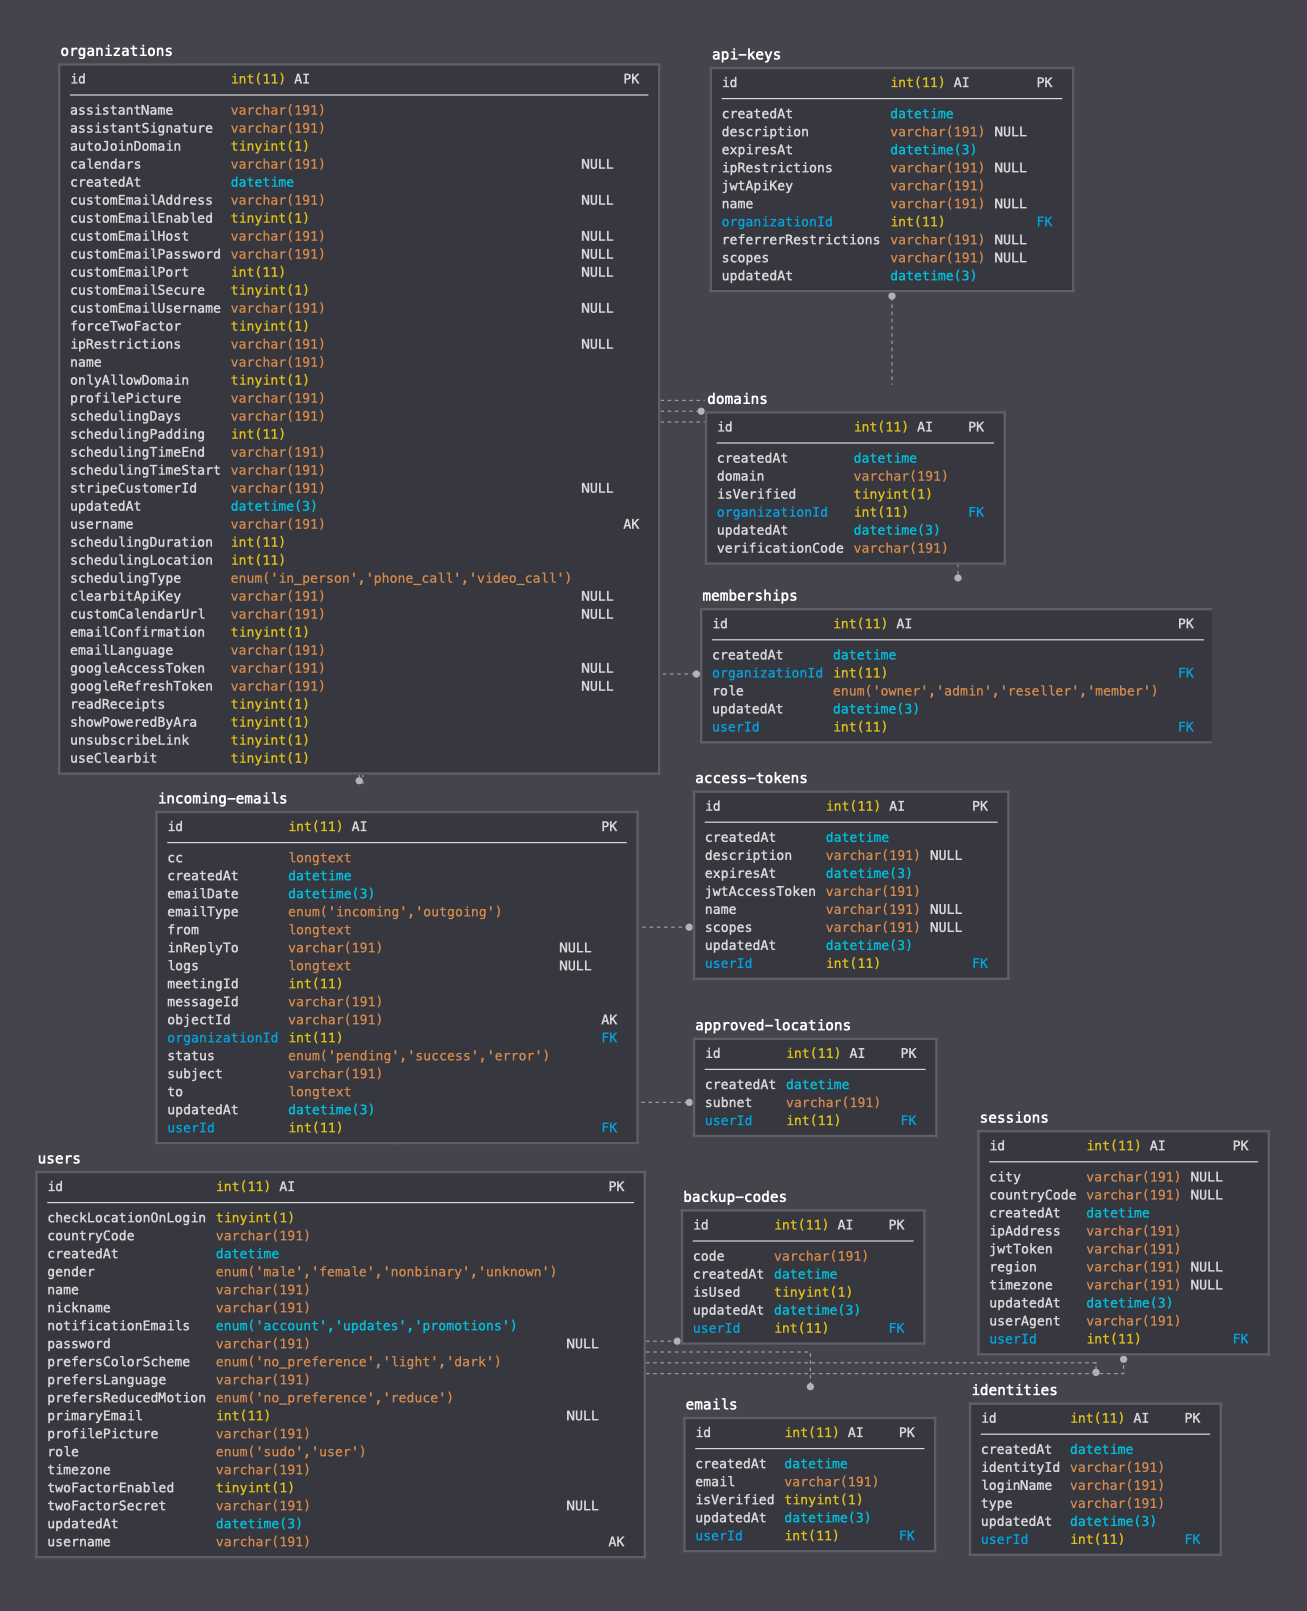
\includegraphics[width=1.15\textwidth]{database-schema.png}}%
  \caption{Database Entity Relationship Diagram}
\end{figure}

\newpage

\bibliography{citations}

\paragraph{License} This work is licensed under a Creative Commons Attribution 4.0 International License (CC BY 4.0). The source code of this research paper is available on \url{https://github.com/AnandChowdhary/bsc-thesis}.

\end{document}